\part[Excursion into Branching Logic]{Excursion Into \\ Branching Logic \\ \ \\ \LARGE Approaches to \CTLstar Synthesis}
%\part{Two Approaches to Synthesis from \CTLstar}

\section*{Overview of Part I}\label{chap:ctlstar:overview}

The reactive synthesis problem was introduced by Alonzo Church~\cite{Church63}.
Given a specification as a formula in Monadic Second Order Logic of One Successor (MSO),
the question is to produce a circuit such that \emph{all} its behaviors satisfy the formula.
Later Pnueli introduced Linear Temporal Logic (LTL)~\cite{pnueli1977temporal}
and together with Rosner solved the synthesis problem for LTL~\cite{DBLP:conf/popl/PnueliR89}.
Now LTL is the main basic logic for specifications.
Both these logics, MSO and LTL, are \emph{linear}:
they describe the set of behaviours,
but do not allow for specifying \emph{structural} properties of the systems.

To be able to specify structural properties
(and to circumvent a relatively high complexity of the verification wrt.\ LTL),
Emerson and Clarke introduced Computation Tree Logic (CTL)~\cite{ctl-origin}.
Later Emerson and Halpern introduced Computation Tree Star Logic (\CTLstar)~\cite{ctlstar-origin}
that subsumed both CTL and LTL.

Let us briefly compare LTL and \CTLstar.

LTL reasons about \emph{computations}.
The logic has \emph{temporal} operators, e.g., $\G$ (always) and $\F$ (eventually),
and can describe properties like ``every request is eventually granted'':
$\G(r \impl \F g)$.
A system satisfies such an LTL property iff \emph{all} its computations satisfy it.
Thus a system is characterized by its computations.

In contrast, \CTLstar reasons about computation \emph{trees}.
Thus, a system is viewed as a tree (cf.\ set of linear paths for LTL),
and we can get such a tree by unfolding the system.
\CTLstar has---in addition to temporal operators---\emph{path quantifiers}:
$\A$ (on all paths) and $\E$ (there exists a path).
Such path quantifiers allow us to reason about branching structure of trees,
not just about the set of its ``linear'' paths.
For example, the \CTLstar formula ``$\AGEF reset$'' says:
``on all tree paths, from every tree node,
  there should be a path into a node where `reset' holds''.
We cannot express such a property using LTL alone.

This part of the thesis explores synthesis approaches from properties in \CTLstar.
It consists of two chapters.

In Chapter~\ref{chap:bosy:ctlstar}
we introduce two approaches to synthesis from \CTLstar.
Both approaches follow the Bounded Synthesis approach
introduced by Finkbeiner and Schewe~\cite{BS}.
In Bounded Synthesis, we repeatedly search for a system of increasing sizes,
until we find a solution.
Bounded Synthesis is very flexible and can be easily adapted
to do e.g. distributed synthesis.
We extend Bounded Synthesis to specifications in \CTLstar and beyond.

The disadvantage of Bounded Synthesis is that it is susceptible to system size:
it works well when the specification admits a small implementation,
but less well when no small implementation exists.
The same holds for our \CTLstar Bounded Synthesis.

In Chapter~\ref{chap:ctl-via-ltl}, partly to overcome this disadvantage,
we introduce a reduction of the \CTLstar synthesis problem to the LTL synthesis problem.
After applying the reduction, any \emph{LTL} synthesiser can do $CTL^*$ synthesis.
Notice that for model checking such a reduction is impossible---%
\CTLstar is more expressive than LTL.
Yet, in synthesis we control the system structure,
which enables the reduction.
The \CTLstar-via-LTL synthesis approach preserves the problem complexity,
although it might increase the size of a system.

The approaches differ in how they ensure the satisfaction of existential \CTLstar subformulas
(recall that universal \CTLstar subformulas, just like LTL, talk about system paths as a whole,
 while existential \CTLstar subformulas specify the existence of a system path).
Recall from Section~\ref{defs:bounded_synthesis} that
bounded synthesis encodes the LTL synthesis problem into the SMT satisfaction problem.
The SMT constraints annotate the states of a \emph{product}
(of a yet unknown system with an automaton expressing a given \CTLstar formula)
with information that ensures that all lassos in the product are not ``bad'' (for universal subformulas)
and that there are ``good'' lassos (for existential subformulas).
In contrast, \CTLstar-via-LTL synthesis produces an LTL formula that
talks about \emph{system} paths and has no direct access to the product.
Hence we move annotations into a system which may increase its size.

This thesis part is organized as follows.
In the next Chapter~\ref{chap:defs} we introduce the definitions
which are used in both chapters.
Chapter~\ref{chap:bosy:ctlstar} focuses on extensions of Bounded Synthesis to \CTLstar,
while Chapter~\ref{chap:ctl-via-ltl} describes the \CTLstar-to-LTL synthesis reduction.
Both chapters depend on the definitions section,
but are independent of each other.


\newcommand{\nocontentsline}[3]{}
\newcommand{\toclesslab}[3]{\bgroup\let\addcontentsline=\nocontentsline#1{#2\label{#3}}\egroup}

%\toclesslab\section{Preliminaries}{chap:defs}
\chapter{Common Definitions for Part I}\label{chap:defs}
Notation:
$\bbB = \{\true,\false\}$ is the set of Boolean values,
$\bbN$ is the set of natural numbers (excluding $0$),
$\bbN_0 = \bbN\cup\{0\}$,
$[k]$ is the set $\{i \in \bbN \| i \leq k\}$
and $[0,k]$ is the set $[k] \cup \{0\}$ for $k \in \bbN$.

The powerset of $A$ is denoted by $2^A$.
We often write $(a,x)$ instead of $a \cup x$ (that is from $2^{A \cup X}$),
and $a \cup x$ instead of $(a,x)$ (that is from $2^A \times 2^X$),
when $a \in 2^A$, $x \in 2^X$ and $A \cap X = \emptyset$.

We denote substitution by the symbol $\mapsto$.
E.g., $(a \land b) [a \mapsto x]$ is $x \land b$.

All systems and automata are finite,
paths are infinite,
and trees have only infinitely long paths but are finitely-branching---%
unless explicitly stated.


\toclesslab\section{Moore Systems}{defs:moore-systems}
%\section{Moore Systems}\label{defs:moore-systems}

A \emph{(Moore) system} $M$ is a tuple
$(I, O, T, t_0, \tau, out)$
where
$I$ and $O$ are disjoint sets of input and output variables,
$T$ is the set of states, $t_0 \in T$ is the initial state,
$\tau: T \times 2^I \to T$ is a transition function,
$out: T \to 2^O$ is the output function that
labels each state with a set of output variables.
Note that systems have no dead ends and have a transition for every input.
We write $t \trans{io} t'$ when $t' = \tau(t,i)$ and $out(t) = o$.
We abuse the notation and define $\tau(t,w)$ for $w_1 w_2 ... w_n \in (2^I)^+$
to be the system state $t_n$ such that $t_0 \trans{io_0} t_1 \trans{io_1} ... \trans{io_{n-1}} t_n$,
i.e., $\tau(t,w)$ is the state where the system ends after reading the word $w$,
when starting from the initial state.

A \emph{system path} is a sequence $t_1 t_2 ... \in T^\omega$
such that for every $i\in \bbN$ there is $e \in 2^I$ with $\tau(t_i,e) = t_{i+1}$.
An \emph{input-labeled system path} is a sequence $(t_1,e_1) (t_2,e_2) ... \in (T\times 2^I)^\omega$
where $\tau(t_i,e_i) = t_{i+1}$ for every $i\in \bbN$.
We sometimes use notation $t_1 \trans{e_1} t_2 \trans{e_2} t_3 ...$
to describe the input-labeled system path $(t_1,e_1) (t_2,e_2) ...$.
A \emph{system computation starting from $t_1 \in T$} is a sequence $(o_1\cup e_1) (o_2\cup e_2) ... \in (2^{I\cup O})^\omega$
for which there exists an input-labeled system path $(t_1,e_1) (t_2,e_2) ...$ 
and $o_i=out(t_i)$ for every $i \in \bbN$.
We write \emph{system computation} to mean system computation starting from the initial state.
Note that since systems are Moore,
the output $o_i$ cannot ``react'' to input $e_i$---%
the outputs are ``delayed'' with respect to inputs.

\begin{remark}\label{rem:inputs-shift}
There are two ways to group inputs and outputs into computations.
The first way is to introduce an initial transition $\tau_I: 2^I \to T$
instead of using the initial state $t_0$.
Then the input-labeled system path $\trans{e_1} t_1 \trans{e_2} t_2 \trans{e_3} t_3 ...$
corresponds to the computation $(e_1, out(t_1)) (e_2, out(t_2)) (e_3, out(t_3)) ...$.
Another way is to avoid using the initial transition---use the initial state $t_0$ instead---and ``shift'' inputs and outputs.
Then an input-labeled system path $t_0 \trans{e_1} t_1 \trans{e_2} t_2 ...$
corresponds to the computation $(out(t_0), e_1) (out(t_1), e_2) ...$.
We use the second approach.
\end{remark}


\ak{add example}

\toclesslab\section{Trees}{defs:trees}
%\section{Trees}\label{defs:trees}

A \emph{(infinite) tree} is a tuple $(D, L, V \subseteq D^*, l:V \to L)$,
where
\li
\- $D$ is the set of directions (in our case, finite),
\- $L$ is the set of node labels (in our case, finite),
\- $V$ is the (infinite) set of nodes satisfying:
   (i) $\epsilon \in V$ is called the root (the empty sequence),
  (ii) $V$ is closed under prefix operation (i.e., every node is connected to the root),
 (iii) for every $n \in V$ there exists a $d \in D$ such that $n\cdot d \in V$
       (i.e., there are no leafs),
\- $l$ is the node labeling function.
\il
A tree $(D,L,V,l)$ is \emph{exhaustive} iff $V=D^*$.
A tree is \emph{non-labeled} iff $|L|=1$ and then we omit $L$ and $l$.

A \emph{tree path} is a sequence $n_1 n_2 ... \in V^\omega$,
such that, for every $i$, there is $d \in D$ such that $n_{i+1} = n_i \cdot d$.

%An \emph{$L$-labeled $D$-directed tree} is a tuple $(V,l)$, where
%$V=D^*$ is the (infinite) set of tree nodes
%and $\epsilon \in V$ (the empty sequence) is called the root node,
%$l: V \to L$ is a labeling function.
%An \emph{(infinite) tree path} is a sequence $n_1 n_2 ... \in V^\omega$,
%such that, for every $i$, there is $d \in D$ and $n_{i+1} = n_i \cdot d$.

In contexts where $I$ and $O$ are inputs and outputs,
we call an exhaustive tree $(D,L,V,l)$
a \emph{computation tree},
where $D=2^I$, $L=2^O$, $V=D^*$, and $l:V \to \O$.
We omit $D$ and $L$ when they are clear from the context.

With every system $M=(I, O, T, t_0, \tau, out)$ we associate
the computation tree $(D, L, V, l)$ such that, for every $n\in V$:
$l(n)=out(\tau(t_0,n))$.
We call such a tree a \emph{system computation tree}.

A computation tree is \emph{regular}
iff it is a system computation tree for some (finite) system.

\ak{example}


\section*{Two Views on the System}\label{defs:two-views-on-system}

Later we introduce logics \CTLstar and LTL to distinguish correct from buggy systems.
The two logics look at systems from two sides.

On one side,
we can associate with a system $M$
a set of its computations $b(M) \subseteq (2^{I\cup O})^\omega$.
A formula $\varphi$ in Linear Temporal Logic (LTL) (introduced later)
describes a set of infinite words $L(\varphi)$.
Thus, we can use an LTL formula to specify all correct computations.
Then a system $M$ is correct wrt.\ LTL formula $\varphi$
iff $b(M) \subseteq L(\varphi)$,
i.e., all system computations satisfy $\varphi$.

On the other side, we might want to specify structural properties of systems.
E.g.,
whether from every system state
we can branch into a state satisfying $p$ and
we can branch into a state satisfying $\neg p$.
In this case, characterizing a system by its set of computations---e.g. using LTL---is not possible.
Instead, we associate with a system its computation tree.
A formula $\Phi$ in Computation Tree Logic (defined later)
describes a set of computation trees $L(\Phi)$.
Thus, we can use such a formula to describe a set of all correct computation trees.
Then a system $M$ is correct wrt.\ $\Phi$ iff $(V,l) \in L(\Phi)$,
i.e., the system computation tree satisfies $\Phi$.


\toclesslab\section{Logics: \CTLstar with Inputs and LTL}{defs:ctlstar}
%\section{Logics: \CTLstar with Inputs and LTL}\label{defs:ctlstar}

\subsection*{\CTLstar with inputs (release PNF)}

Fix two disjoint sets: inputs $I$ and outputs $O$.
Below we define \CTLstar with inputs, in release positive normal form%
\footnote{This form is sometimes called negation normal form.
  For the name, we follow~\cite{PrinciplesMC}.
  Note that without the release operator $\R$%
  ---the dual of the until operator $\U$---%
  the logic is less expressive due to the restriction on negations.
  That explains the name ``release PNF''.}.
The definition differentiates inputs and outputs (see Remark~\ref{rem:ctlstar-subtle}).

\parbf{Syntax}
\emph{State formulas} have the grammar:
$$
\Phi = \true \| \false \|
       o \| \neg o \| \Phi \land \Phi \| \Phi \lor \Phi \|
       \A \varphi \| \E \varphi
$$
where $o \in O$ and $\varphi$ is a path formula. \emph{Path formulas} are defined by the grammar:
$$
\varphi = \Phi \|
      i \| \neg i \|
      \varphi \land \varphi \| \varphi \lor \varphi \|
      \X \varphi \|
      \varphi \U \varphi \|
      \varphi \R \varphi,
$$
where $i \in I$.
The temporal operators $\G$ and $\F$ are defined as usual.

The above grammar describes the \CTLstar formulas in positive normal form.
The general \CTLstar formula
(in which negations can appear anywhere)
can be converted into the formula of this form with no size blowup,
using the equivalence $\neg (a \U b) \equiv \neg a \R \neg b$ and some others.

\parbf{Semantics}
We define the semantics of \CTLstar with respect to a computation tree $(V,l)$
(where $D=2^I$ and $L=2^O$).
The definition is very similar to the standard one~\cite{PrinciplesMC},
except for a few cases involving inputs
(marked with ``+'').

Let $n \in V$ and $o \in O$.
Then:
\li
\- $n \not\models \Phi$ iff $n \models \Phi$ does not hold,
\- $n \models \true$ and $n \not\models \false$,
\- $n \models o$ iff $o \in l(n)$, $n \models \neg o$ iff $o \not\in l(n)$,
\- $n \models \Phi_1 \land \Phi_2$ iff $n \models \Phi_1$ and $n \models \Phi_2$.
   Similarly for $\Phi_1\lor\Phi_2$.
\- $n \models \A \varphi$ iff for all tree paths $\pi$ starting from $n$:
   $\pi \models \varphi$.
   For $\E\varphi$, replace ``for all'' with ``there exists''.
\il

Let $\pi = n_1 n_2 ... \in V^\omega$ be a tree path,
$i \in I$, and $n_2 = n_1 \cdot e$ where $e \in \I$.
For $k \in \bbN$, define $\pi_{[k:]} = n_k n_{k+1} ...$,
i.e., the suffix of $\pi$ starting in $n_k$.
Then:
\li
\- $\pi \models \Phi$ iff $n_1 \models \Phi$,
\-[+] $\pi \models i$ iff $i \in e$, $\pi \models \neg i$ iff $i \not\in e$,
\- $\pi \models \varphi_1 \land \varphi_2$ iff $\pi \models \varphi_1$ and $\pi \models \varphi_2$.
   Similarly for $\varphi_1 \lor \varphi_2$.
\- $\pi \models \X \varphi$ iff $\pi_{[2:]} \models \varphi$,
\- $\pi \models \varphi_1 \U \varphi_2$ iff
   $\exists l\in\bbN: (\pi_{[l:]} \models \varphi_2 \land \forall m \in [1,l-1]: \pi_{[m:]} \models \varphi_1)$,
\- $\pi \models \varphi_1 \R \varphi_2$ iff
   $(\forall l\in\bbN: \pi_{[l:]} \models \varphi_2) \lor 
    (\exists l\in\bbN: \pi_{[l:]} \models \varphi_1 \land \forall m\in [1,l]: \pi_{[m:]} \models \varphi_2)$.
\il

A \emph{computation tree $(V,l)$ satisfies a \CTLstar state formula $\Phi$},
written $(V,l) \models \Phi$,
iff the root node satisfies it.
A \emph{system $M$ satisfies a \CTLstar state formula $\Phi$},
written $M \models \Phi$,
iff its computation tree satisfies it.

\begin{remark}[Subtleties]\label{rem:ctlstar-subtle}
Note that $(V,l) \models i\land o$ is not defined,
since $i \land o$ is not a state formula.
Let $r \in I$ and $g \in O$.
By the semantics, $\E r \equiv \true$ and $\E \neg r \equiv \true$,
while $\E g \equiv g$ and $\E \neg g \equiv \neg g$.
These facts are the consequences of the way we group inputs with outputs
(see also Remark~\ref{rem:inputs-shift}).
\end{remark}


\subsection*{LTL}
The syntax of LTL formulas (in general form) is:
$$
\phi = \true \| p \| \neg p \| \phi \land \phi \| \neg \phi \| \phi \U \phi \| \X \phi,
$$
where $p \in I \cup O$.
The temporal operators $\G$ and $\F$ are defined as usual,
and $\false = \neg \true$.
The semantics is standard (see, e.g., \cite{PrinciplesMC}).
A computation tree $(V,l)$ satisfies an LTL formula $\phi$,
written $(V,l) \models \phi$,
iff all tree paths starting in the root satisfy it.
A system satisfies an LTL formula iff its computation tree satisfies it
(equivalently, every system computation starting from the initial state
 satisfies the LTL formula).


\toclesslab\section{Tree Automata}{defs:tree-automata}
%\section{Tree Automata}\label{defs:tree-automata}

Tree automata consume infinite trees and output ``accept'' or ``reject''.
Since every Moore system has a corresponding computation tree,
tree automata can be used to differentiate buggy Moore machines from correct ones.
Also, \CTLstar can be translated into a special type of alternating tree automata.
Thus, tree automata are the excellent tool for model checking and synthesis.

We start with a general definition of alternating tree automata,
then introduce different acceptance conditions,
then introduce alternating hesitant tree automata.

\parit{Notation ${\cal B}^+(S)$}
For a finite non-empty set $S$,
let ${\cal B}^+(S)$ be the set of all positive Boolean formulas over elements of $S$,
i.e., every such a formula $\phi$ has the syntax:
$\phi = e \| \phi \land \phi \| \phi \lor \phi$, where $e \in S$.
Note that $\false \not\in {\cal B}^+(S)$ and $\true \not\in {\cal B}^+(S)$.
As we will see later, these are not limitations in our context.
Also, since the set $S$ is finite,
any Boolean formula over atoms in $S$ and which is semantically different from $\true$ and $\false$
is equivalent to some formula in ${\cal B}^+(S)$.
Furthermore,
every formula $\phi \in {\cal B}^+(S)$ can be rewritten into formula $\phi' \in {\cal B}^+(S)$ in disjunctive normal form (DNF)
or into formula $\phi'' \in {\cal B}^+(S)$ in conjunctive normal form (CNF).
We assume that formulas in ${\cal B}^+(S)$ (and thus CNF and DNF formulas)
have neither redundant atoms, conjuncts, nor disjuncts.
%Finally,
%every formula $\phi \in {\cal B}^+(S)$ can be seen as a non-empty set of non-empty sets of atoms from $S$

%For a finite set $S$,
%let ${\cal B}^+(S)$ denote the set of all positive Boolean formulas over elements of $S$ or $\true$,
%i.e., every such a formula $\phi$ has the syntax:
%$\phi = \true \| e \| \phi \land \phi \| \phi \lor \phi$, where $e \in S$.
%Note that $\false \not\in {\cal B}^+(S)$.


\subsection*{Alternating tree automata}

An \emph{alternating tree automaton} is a tuple
$(\Sigma, D, Q, q_0, \delta, acc)$,
where $\Sigma$ is the set of node propositions,
$D$ is the set of directions, $q_0 \subseteq Q$ is the initial state,
$\delta: Q \times \Sigma \to \mathcal{B}^+(D \times Q)$
is the transition relation,
and $acc: Q^\omega \to \bbB$ is an acceptance condition.
For simplicity we assume that $\delta$ is total wrt.\ directions.
Thus, it is worth noting about $\delta(q,\sigma)$, for every $(q,\sigma) \in Q\times\Sigma$:
\li
\- if we rewrite $\delta(q,\sigma)$ into DNF,
   then each conjunct mentions each direction at least once (``totalness'' wrt.\ directions).
\- $\delta(q,\sigma) \neq \false$ and $\delta(q,\sigma) \neq \true$.
   These are not limitations,
   because we can emulate $\true$ and $\false$ by introducing additional states and modifying $acc$.
\il
The above means that $\delta$ has a transition for every possible argument and direction.

Fix two disjoint sets, inputs $I$ and outputs $O$.

Tree automata consume exhaustive trees like $(D, L=\Sigma, V=D^*, l:V \to \Sigma)$
and produce run-trees.

A \emph{run-tree} of an alternating tree automaton
$(\Sigma=2^O, D=2^I, Q, q_0, \delta, acc)$
on a computation tree $(V=(2^I)^*, l:V \to \O)$
is a tree
with directions $2^I \times Q$,
labels $V \times Q$,
nodes $V' \subseteq (2^I \times Q)^*$,
labeling function $l'$
such that
\li
\- $l'(\epsilon) = (\epsilon, q_0)$,
\- if $v \in V'$ with $l'(v) = (n,q)$, then:\\
   there exists $\{(d_1,q_1),...,(d_k,q_k)\}$ that satisfies $\delta(q, l(n))$
   and $n \cdot (d_i, q_i) \in V'$ for every $i \in [1,k]$.
\il
Intuitively,
we run the alternating tree automaton on the computation tree:
\li
\-[(1)]
   We mark the root node of the computation tree with the automaton initial state $q_0$.
   We say that initially, in the node $\epsilon$,
   there is only one copy of the automaton and it has state $q_0$.
\-[(2)]
   We read the label $l(n)$ of the current node $n$ of the computation tree
   and consult the transition function $\delta(q,l(n))$.
   The latter gives a set of conjuncts of atoms of the form $(d',q') \in D\times Q$.
   We nondeterministically choose one such conjunction $\{(d_1,q_1), ..., (d_k,q_k)\}$
   and send a copy of the alternating automaton into each direction $d_i$ in the state $q_i$.
   Note that we can send up to $|Q|$ copies of the automaton into one direction
   (but into different automaton states).
   That is why a run-tree defined above has directions $2^I\times Q$
   rather than $2^I$.
\-[(3)]
   We repeat step (2) for every copy of the automaton.
   As a result we get a run-tree:
   a tree labeled with nodes of the computation tree and
   states of the automaton.
\il

A \emph{run-tree is accepting}
iff every run-tree path starting from the root is accepting.
A run-tree path $v_1 v_2 ...$ is accepting
iff $acc(q_1q_2...)$ holds ($acc$ is defined later),
where $q_i$ for every $i\in \bbN$ is the automaton state part of $l'(v_i)$.
Note that every run-tree path is infinite.
(In particularly, we do not have \emph{finite} paths that end with $\true$ nor $\false$,
 by definition of $\delta:Q\times\Sigma\to{\cal B}^+(D\times Q)$.)

An \emph{alternating tree automaton $A=(\Sigma=2^O, D=2^I, Q, q_0, \delta, acc)$
accepts a computation tree $(V=(2^I)^*, l:V \to \O)$},
written $(V,l) \models A$,
iff
the automaton has an accepting run-tree on that computation tree.
An alternating tree automaton is \emph{non-empty} iff there exists a computation tree accepted by it.

Similarly,
\emph{a Moore system $M=(I, O, T, t_0, \tau, out)$
is accepted
by the alternating tree automaton $A=(\Sigma=2^O, D=2^I, Q, q_0, \delta, acc)$},
written $M \models A$,
iff $(V,l) \models A$,
where $(V=(2^I)^*,l:V\to 2^O)$ is the system computation tree.

Let us define different variations of an acceptance condition $acc: Q^\omega \to \bbB$.
For a given infinite sequence $\pi \in Q^\omega$,
let $\Inf(\pi)$ be the elements of $Q$ appearing in $\pi$ infinitely often.
Then:
\li
\- \emph{B\"uchi acceptance} is defined by a set $F \subseteq Q$:
   $acc(\pi)$ holds iff $\Inf(\pi) \cap F \neq \emptyset$.
   We often call the states of $F$ \emph{accepting}.
\- \emph{Co-B\"uchi acceptance} is defined by a set $F \subseteq Q$:
   $acc(\pi)$ holds iff $\Inf(\pi) \cap F = \emptyset$.
   We often call the states of $F$ \emph{rejecting}.
\- \emph{Streett acceptance} is defined by pairs $\{(A_i\subseteq Q,G_i \subseteq Q)\}_{i\in[k]}$:
   $acc(\pi)$ holds
   iff
   $\forall i \in [k]: \Inf(\pi)\cap A_i \neq \emptyset \impl \Inf(\pi) \cap G_i\neq\emptyset$.
\- \emph{Rabin acceptance} is defined by pairs $\{(F_i,I_i)\}_{i \in [k]}$:
   $acc(\pi)$ holds
   iff
   $\exists i \in [k]: \Inf(\pi) \cap F_i = \emptyset \land \Inf(\pi) \cap I_i \neq \emptyset$.
\- \emph{Parity acceptance} is defined by a priority function
   $p: Q \to [0,k]$:
   $acc(\pi)$ holds iff the minimal priority appearing infinitely often in $p(\pi)$ is even.
\il
In addition to the above acceptance conditions,
we define generalized versions.
Generalized B\"uchi acceptance condition is defined by a set $\{F_i\}_{i \in [k]}$:
$acc(\pi)$ holds iff the B\"uchi condition holds wrt.\ every $F_i$ where $i \in [k]$.
Similarly define Generalized co-B\"uchi%
\footnote{We stress that, in our work, Generalized co-B\"uchi
  for a set $\{F_i\}_{i \in [k]}$ means:
  $acc(\pi)$ holds iff the co-B\"uchi condition holds wrt.\ \emph{every} $F_i$ where $i \in [k]$.
  But often Generalized co-B\"uchi acceptance means that
  \emph{there exists} $F_i$ that is visited finitely often where $i \in [k]$.%
},
Streett, Rabin, and Parity conditions.

\subsection*{Nondeterministic and universal tree automata}

Depending on the form of $\delta(q,\sigma)$ (for every $(q,\sigma) \in Q\times\Sigma$),
we distinguish the following special cases of alternating tree automata.
\li
\- \emph{Universal} tree automata:
   $\delta(q,\sigma)$ is a conjunction of variables of $Q\times D$,
   where each direction is mentioned at least once.
\- \emph{Deterministic} tree automata:
   $\delta(q,\sigma)$ is a conjunction of variables of $Q \times D$ and
   each direction is mentioned exactly once.
\- \emph{Nondeterministic} tree automata:
   let $\delta(q,\sigma)$ be rewritten in DNF.
   Then each conjunct mentions each direction exactly once.
\il

\ak{state known facts: (1) non-empty iff regularly non-empty, (2) non-empt complexity, (3) conversion of \CTLstar into AHTs, (4) determinisation?}

\subsection*{Alternating hesitant tree automata (AHT)} \label{page:defs:aht}

An \emph{alternating hesitant tree automaton (AHT)} is an alternating tree automaton
$(\Sigma, D, Q, q_0, \delta, acc)$
with the following acceptance condition and structural restrictions.
The restrictions reflect the fact that AHTs are tailored for \CTLstar formulas.
\li 
\- $Q$ can be partitioned into $Q^N_1,\dots ,Q^N_{k_N}$, $Q^U_1,\dots
,Q^U_{k_U}$, where superscript $N$ means
nondeterministic and $U$ means universal.
Let $Q^N = \bigcup Q^N_i$ and $Q^U = \bigcup Q^U_i$.
(Intuitively,
 nondeterministic state sets describe \E-quantified subformulas of the \CTLstar formula,
 while universal state sets describe \A-quantified subformulas.)

\- There is a partial order on $\{Q^N_1,\dots ,Q^N_{k_N},Q^U_1,\dots , Q^U_{k_U}\}$.
   (Intuitively, this is because state subformulas can
    be ordered according to their relative nesting.)

\- The transition function $\delta$ satisfies: for every $q \in Q$, $a \in \Sigma$
   \li
   \- if $q \in Q^N_i$, then:
      $\delta(q,a)$ contains only disjunctively related\footnotemark[1] elements of $Q^N_i$;
      every element of $\delta(q,a)$ outside of $Q^N_i$ belongs to a lower set;
   \- if $q \in Q^U_i$, then:
      $\delta(q,a)$ contains only conjunctively related\footnotemark[1] elements of $Q^U_i$;
      every element of $\delta(q,a)$ outside of $Q^U_i$ belongs to a lower set.
   \il
   \ak{figure of disj-conj related sets: and why?!}
\il
\footnotetext[1]{In a Boolean formula, atoms $E$ are disjunctively [conjunctively] related
  iff the formula can be written into DNF [CNF] in such a way that each cube [clause] has at most one element from $E$.}

Finally, $acc: Q^\omega \to \bbB$ of AHTs is defined by a set $Acc \subseteq Q$:
$acc(\pi)$ holds for $\pi=q_1q_2...\in Q^\omega$ iff one of the following holds.
\li
\- The sequence $\pi$ eventually stays in some $Q^U_i$ and
   $\Inf(\pi) \cap (Acc\cap Q^U) = \emptyset$
   (co-B\"uchi acceptance).
   Let us denote $F = Acc \cap Q^U$.
\- The sequence $\pi$ eventually stays in some $Q^N_i$ and
   $\Inf(\pi) \cap (Acc \cap Q^N) \neq \emptyset$
   (B\"uchi acceptance).
   Let us denote $I = (Acc \cap Q^N) \cup (Q^U \!\setminus\! Acc)$.
\il
Due to the restrictions on the structure of hesitant automata,
this acceptance is equivalent to the Rabin acceptance with one pair $(F,I)$.

\ak{examples}


\toclesslab\section{Word Automata}{defs:word-automata}
%\section{Word Automata}\label{defs:word-automata}

In contrast to tree automata that consume infinite trees,
word automata consume infinite words.
Every LTL formula can be translated into a word automaton,
but a \CTLstar formula, in general, cannot.
This is because a \CTLstar formula describes a set of trees,
while an LTL formula describes a set of words.

We start with alternating word automata.
Such automata can concisely represent LTL formulas
(without incurring an exponential blow-up in its size).
Then we define two specializations: nondeterministic and universal word automata.
Such automata are often used as input to synthesis algorithms,
because they are simpler to work with
(although translation of an LTL formula into such an automaton can incur
 and exponential blow-up).
Finally, we define alternating hesitant word automata.
They are useful for model checking and synthesis from AHTs
(and thus from \CTLstar formulas).

\subsection*{Alternating word automata}
%How a tree automaton $(\Sigma, D, Q, q_0, \delta, acc)$ looks like when $|D|=1$
%(thus trees have one branch only)?
%The transition function becomes
%$\delta: Q\times\Sigma \to {\cal B}^+(Q)$.

%An \emph{alternating word automaton $(\Sigma, Q, q_0, \delta, acc)$}
%is an alternating tree automaton $(\Sigma, D, Q, q_0, \delta, acc)$ with $|D|=1$.
%Run tree becomes run path.
%The difficulty arises when defining $M \models A$, where $A$ is a word automaton.
%We cannot define $M \models A$ iff $(V,l) \models A$,
%since we requested $A$ to have only one direction ($|2^I|=1$),
%while system can have $|I|>0$.
%We can overcome this by defining $\Sigma=2^I\cup 2^O$,
%but then we need to consider non-deterministic systems.
%
%Usually we use $D$ to describe inputs: $D=2^I$.
%Although now we require $|D|=1$, we can still use word automata to
%distinguish correct from buggy Moore systems.
%The idea is to consider $\Sigma=2^I \cup 2^O$
%(cf. $\Sigma=2^O$ in the previous section).

\begin{remark}[Re-using definitions from tree automata]
An infinite word can be viewed as a tree with a single branch.
Thus it is tempting to derive definitions for word automata from those of tree automata.
Without additional tricks this will not work for the following reason.
In our work, branching degree of every computation tree is, by definition, $|2^I|$.
Thus, considering only single-branch trees is equivalent to
having systems with no inputs: $|2^I|=1 \Iff |I|=0$.
But we are interested in the general case: $|I| \in \bbN_0$.
(To reuse definitions, we could move the inputs into the outputs,
 consider nondeterministic systems without edge labels,
 and require that each state has a successor containing a label $e$, for every $e \in 2^I$.)
\end{remark}

An \emph{alternating word automaton} is a tuple $(\Sigma, Q, q_0, \delta, acc)$
where $\Sigma$ is an alphabet, $Q$ is a set of states, $q_0 \in Q$ is initial,
$\delta: Q \times \Sigma \to {\cal B}^+(Q)$ is a transition function,
and $acc:Q^\omega \to \bbB$ is a path acceptance condition.
Note that $\delta(q) \neq \false$ and $\delta(q) \neq \true$ for every $q\in Q$,
i.e., there is a successor state for every letter.
These are not real limitations, they are in place to simplify definitions.
% ak: not sure if we use this restriction

Given a word $w = a_1 a_2 ... \in \Sigma^\omega$,
let $\Pref(w) = \{\epsilon, a_1, a_1 a_2, a_1 a_2 a_3, ...\}$
denote the set of all its prefixes (including the empty prefix).
Also,
for a finite non-empty word $w \in \Sigma^+$,
let $last(w)$ denote its last letter.

A \emph{run-tree} of an alternating word automaton
$(\Sigma, Q, q_0, \delta, acc)$
on an infinite word $w = a_1 a_2 ... \in \Sigma^\omega$
is a tree
with directions $Q$,
labels $\Pref(w) \times Q$,
nodes $V' \subseteq (\Sigma \times Q)^*$,
labeling function $l': V' \to \Pref(w) \times Q$
such that
\li
\- $l'(\epsilon) = (\epsilon, q_0)$,
\- if $v \in V'$ with $l'(v) = (p,q)$, then:\\
   there exists $\{q_1,...,q_k\}$ that satisfies $\delta(q, last(p))$
   and $p \cdot q_i \in V'$ for every $i \in [1,k]$.
\il
This definition coincides with the definition of run-trees of tree automata
when restricted to trees with a singe path.

A \emph{run-tree is accepting}
iff every run-tree path starting from the root is accepting.
A run-tree path $v_1 v_2 ...$ is accepting
iff $acc(q_1 q_2 ...)$ holds,
where $q_i$, for every $i$, is an automaton state of the label $l'(v_i)$.

An \emph{alternating word automaton $A=(\Sigma, Q, q_0, \delta, acc)$
accepts an infinite word $w=a_1 a_2... \in \Sigma^\omega$},
written $w \models A$,
iff
the automaton has an accepting run-tree on the word.
An alternating word automaton is \emph{non-empty}
iff there exists an infinite word accepted by it.

So far we re-used definitions from Section~\ref{defs:tree-automata},
but now we depart.

In Section~\ref{defs:ctlstar} about \CTLstar, we introduced two path quantifiers:
$\A$ (on all paths) and $\E$ (there exists a path).
Accordingly, we define $M\models \A(A)$ and $M \models \E(A)$:
$M \models \E(A)$ iff there is a system computation accepted by the automaton;
$M \models \A(A)$ iff every system computation is accepted by the automaton.

\begin{remark}[Tree automata vs. Word automata]
Consider \CTLstar formula $\EX g \land \EX \neg g$,
outputs $O = \{g\}$, inputs $I = \{r\}$.
No alternating \emph{word} automaton, when prefixed with $\E$ or $\A$,
can describe this language,
while there is an alternating \emph{tree} automaton for it\ak{see Fig.XXX}.
\end{remark}

\subsection*{Nondeterministic and universal word automata}

We now look closer at nondeterministic and universal word automata.
Their definitions coincide
with those for tree automata when assuming the single direction,
but for clarity we recall them here.

Depending on the form of $\delta(q,a)$ (for every $(q,a) \in Q\times\Sigma$),
we distinguish:
\li
\- \emph{Deterministic} word automata: $\delta(q,a)$ is a single state.
   There is no choice: we know exactly into which state to proceed
   from $q$ when reading $a$.
   Thus, a run-tree degenerates into a line.
\- \emph{Nondeterministic} word automata: $\delta(q,a)$ is a (non-empty) disjunction of states.
   We reading $a$ in state $q$, we choose one of the states and proceed.
   A run-tree degenerates into a line.
\- \emph{Universal} word automata: $\delta(q,a)$ is a conjunction of states
   $q_1\land...\land q_k$ where $k \geq 1$.
   Thus, when reading $a$ we send one copy of the automaton into every $q_1 ... q_k$.
   A run-tree is indeed a tree.
\il
In all the cases above,
the transition function can be expressed as $\delta: Q\times\Sigma \to 2^Q \setminus \{\emptyset\}$.
We often use this notation instead of $\delta: Q\times\Sigma \to {\cal B}^+(Q)$.


\subsection*{Alternating hesitant word automata (AHW)} \label{page:defs:ahw}

An \emph{alternating hesitant word automaton} (AHW)
$A=(\Sigma, Q, q_0, \delta: Q\times\Sigma \to {\cal B}^+(Q), Acc \subseteq Q)$
is an alternating word automaton with
the similar to AHTs structural restrictions and the same as for AHTs acceptance condition.


\subsection*{Tree variants of word automata} \label{page:defs:tree_variants}

We define the following tree variants, $A_\A$ and $A_\E$, of a word automaton $A$.
Given a nondeterministic word automaton
$A = (2^{I\cup O}, Q, q_0, \delta: Q\times 2^{I\cup O} \to 2^Q, acc)$,
let $A_\E = (2^O, D=2^I, Q,q_0, \delta': Q\times 2^O \to 2^{Q\times D}, acc)$
be the nondeterministic tree automaton defined in the most natural way:
for every $(q,o) \in Q \times 2^O$,
$$
\delta'(q,o) = \bigvee_{d \in D} \delta\big(q,(o,d)\big) \left[q' \mapsto (d,q')\right].
$$
We define $A_\A$ in the same way.

We will use $A_\E$ to talk about
``the product between system $M$ and nondeterministic \emph{word} automaton $A$''.
Since we do not define such a product---it is defined for \emph{tree} automata only---%
we use $A_\E$ instead.
Similarly, when we have universal word automata, we use $A_\A$.

$A_\A$ and $A_\E$ satisfy the following property:
for every system $M$,
\li
\- for universal $A$: $M \models \A(A) ~\Iff~ M \models A_\A$,
\- for nondeterministic $A$: $M \models \E(A) ~\Iff~ M \models A_\E$.
\il

%We mention the important property of AHWs.
%Recall that the states of an AHW can be partitioned into
%``existential'' sets $Q^N_1, ..., Q^N_{k_N}$ and
%``universal'' sets $Q^U_1, ..., Q^U_{k_U}$.
%Such sets are ordered and the transition function ensure the following:
%Every path in every run-tree of the AHW
%gets trapped in some $Q^N_i$ or in $Q^U_j$.
%We use this observation when encoding
%the \CTLstar model checking problem into an SMT query.

%In Section~\ref{defs:model-checking-approach} we use 1-letter AHWs

%\emph{A path in automaton $A$}
%is a sequence $q_0 q_1 ... \in Q^\omega$ starting in the initial state
%such that there exists $a_i \in \Sigma$ for every $i \geq 0$
%such that $(q_i,a_i,q_{i+1}) \in \delta(q_i)$.
%\emph{A sequence $a_0 a_1 \dots  \in \Sigma^\omega$ generates a path}
%$\pi = q_0 q_1\dots $ iff for every $i \geq 0$: $(q_i,a_i,q_{i+1}) \in \delta$.
%A \emph{path $\pi$ is accepted} iff $acc(\pi)$ holds.
%
%We distinguish two types of automata: universal and non-deterministic.
%The type defines when the automaton accepts a given infinite sequence.
%
%A \emph{non-deterministic automaton $A$ accepts an infinite sequence}
%from $\Sigma^\omega$
%iff there exists an accepted path generated by the sequence.
%Universal automata require \emph{all} paths generated by the sequence to be accepted.
%For an automaton $A$, write $L(A)$ for the set of all infinite sequences accepted by $A$.
%Equvalently,
%in both cases:
%an automaton accepts an infinite sequence iff there is an accepting run.


\section*{Automata Abbreviations}\label{defs:automata-abbrv}
We use the standard three letter abbreviation for automata
$$(\{A,U,N,D\}\times\{B,C,S,P,R\}\times\{W,T\}) \cup \{AHT, AHW\}.$$
For example,
NBW means Nondeterministic B\"uchi Word automaton,
UCT means Universal co-B\"uchi Tree automaton,
AHT means Alternating Hesitant Tree automaton.

\toclesslab\section{Approaches to Model Checking}{defs:model-checking-approach}
%\section{Approaches to Model Checking}\label{defs:model-checking-approach}

This section treats the automata-theoretic approach to \CTLstar and LTL model checking~\cite{ATA},
as well as the classical bottom-up approach to \CTLstar model checking~\cite{DBLP:journals/toplas/ClarkeES86}.
Let us start with the definition.

\smallskip
The \emph{model checking problem} is:

\smallskip
\noindent
\emph{%
Given: a Moore system $M$, formula $\Phi$ in some logic\\
Return: does $M \models \Phi$?
}

\smallskip
\noindent
Depending on the logic of $\Phi$,
we have \CTLstar and LTL model checking problems.

\medskip
We now briefly describe the automata-based solution to \CTLstar (and thus LTL)
model checking problem
introduced by Kupferman, Vardi, and Wolper~\cite{ATA}.
The idea is to translate a given formula $\Phi$ into a tree automaton:
\li
\- into AHT, when $\Phi$ is in \CTLstar,
\- into UCT, when $\Phi$ is in LTL.
\il
Then we build the ``product'' of the system and the automaton,
which will be a word automaton (an alternating one for \CTLstar, a universal one for LTL).
Such a word automaton captures the joint behaviours
of the system and the automaton for $\Phi$.
The nice property of the product is that it is empty iff
the system is accepted by the tree automaton for $\Phi$
(equivalently: iff the system satisfies $\Phi$).
Thus, we reduce the model checking problem to checking the non-emptiness
of a word automaton.
Below we define the product.

\subsection*{Product of system and tree automaton}

Let us provide the intuition.
%The product of a system and a tree automaton will allows us
%to reduce the question ``whether the system is accepted by the automaton''
%into the non-emptiness question of the product automaton.

A system $M$ can be seen as a deterministic tree automaton $A_M$
that accepts only its own computation tree.
Then the question of whether the system is accepted
by a given tree automaton $A$
is equivalent to checking whether the intersection $A_M \land A$ is non-empty.
The product of a system $M$ and a tree automaton $A$,
written $M\otimes A$,
can be seen as the intersection tree automaton $A_M \land A$,
from which we remove labels and directions%
\footnote{%
 We can remove labels because,
 for each state of $A_s$,
 the label is uniquely defined---it is $out(t)$ for the corresponding system state $t$.
 We can remove directions,
 because in the non-emptiness check of a 1-letter tree automaton
 we do not distinguish directions.%
}
and which we treat as a \emph{word} automaton.
The important property is that the product $M\otimes A$---a 1-letter alternating word automaton---
is empty iff $A_M \land A$ is empty.

%Then the product of the system and a tree automaton $A$
%is the intersection $A_s \land A$.
%Thus, every transition of the product describes
%both a transition of the system and a transition of the automaton $A$.
%Now let us ask ``Is the automaton $A_s \land A$ non-empty?''
%Since the only computation tree it can accept belongs to the system,
%this question is equivalent to ``$M \in L(A)$?'' (equiv.: ``$M \models A$?'').
%
%If we are interested only in the non-emptiness of $A_s \land A$,
%we can treat it as a \emph{1-letter word} automaton for the following reasons.
%
%Here is why 1-letter alphabet is enough.
%Every system state $t$ has exactly one output label $out(t)$.
%Hence the tree automaton $A_s$, in every its state,
%rejects all output labels except one ($out(t)$, for the corresponding $t$).
%The same holds for the intersection $A_s \land A$.
%Thus, when checking the non-emptiness of $A_s \land A$,
%we have no choice of letters---they are already fixed by the system.

%Here is why we can treat $A_s \land A$ as a \emph{word} automaton.
%With 1-letter alphabet $\Sigma=\{\sigma\}$,
%whe transition function of $A_s \land A$,
%$\delta_{A_s\land A}: Q\times\Sigma \to {\cal B}^+(D \times Q)$
%can be seen as
%$\delta_{A_s\land A}: Q \to {\cal B}^+(D \times Q)$.

A \emph{1-letter alternating hesitant word automaton (1-AHW)} is
an AHW $(Q, q_0, \delta: Q \to \mathcal{B}^+(Q), Acc \subseteq Q)$,
whose alphabet has only one letter (not shown in the tuple).
Informally,
an 1-AHW is an and-or graph of a restricted form
plus a Rabin acceptance condition.

%A \emph{run of a 1-AHW} 
%$(Q, q_0, \delta: Q \to \mathcal{B}^+(Q), Acc \subseteq Q)$
%is a labeled tree defined in a standard way.
%Its nodes are from $Q^*$,
%the root is $q_0$,
%the labeling $l$ maps a node (in $Q^*$) to the last element (in $Q$),
%and for any reachable node, $l(succ(n)) \models \delta(l(n))$ where $l(succ(n))$
%is the set of labels of the successors of node $n$.
%A \emph{run is accepting} if all paths of the tree
%satisfy the acceptance condition.
%A run tree \emph{path satisfies the acceptance condition $Acc$}
%iff one of the following holds:
%\li
%\- the corresponding path in the 1-AHW gets trapped in some $Q^U$
%   and visits $Acc\cap Q^U$ only finitely often, or
%\- the corresponding path in the 1-AHW gets trapped in some $Q^N$ 
%   and visits some state of $Acc \cap Q^N$ infinitely often.
%\il
%Intuitively, the 1-AHW acceptance condition is a mix of B\"uchi
%and co-B\"uchi acceptance conditions.
%It can also be seen as a Rabin acceptance with one pair
%$(F,I)$ where
%$F = Acc \cap Q^U$ and $I = (Acc \cap Q^N) \cup (Q^U\!\setminus\! Acc$).
%
%Note that any path of a run tree of a 1-AHW
%is trapped in some $Q^N_i$ or $Q^U_i$.
%
%The \emph{non-emptiness question of 1-AHW} is
%``does the automaton has an accepting run?''.

A \emph{product} of an AHT
$A\!\!=\!\!(2^O, 2^I, Q, q_0, \delta, Acc)$ and a system $M\!\!=\!\!(I,O,T,t_0,\tau,out)$,
written $M \otimes A$,
is a 1-AHW
${(Q \times T, (q_0,t_0), \Delta, Acc')}$
such that
$${Acc'=\{(q,t) \mid q \in Acc\}}$$
and for every $(q,t) \in Q \times T$:
$$
{\Delta(q,t)=\delta(q,out(t))[(d,q') \mapsto (\tau(t,d),q')]}.
$$
As before, $M \otimes A$ is non-empty iff there exists an infinite word accepted by it.
Since $M \otimes A$ has a one-letter alphabet---let it be $\Sigma = \{l\}$---%
checking the non-emptiness of $M \otimes A$ means checking
whether the infinite word $l^\omega$ is accepted.

Recall that the states of an AHW can be partitioned into
``existential'' sets $Q^N_1, ..., Q^N_{k_N}$ and
``universal'' sets $Q^U_1, ..., Q^U_{k_U}$.
These sets are ordered, and the transition function of the AHW
satisfies the restriction that ensures the following:
every infinite path of the AHW gets trapped in some $Q^N_i$ or $Q^U_j$.

\subsubsection{\CTLstar model checking using the product}

For the general case of \CTLstar formulas and AHTs we know the following.
\begin{proposition}[\cite{ATA}]
A system $M$ is accepted by an AHT $A$ iff their product $M \otimes A$ is non-empty.
\end{proposition}
\begin{corollary}
A system $M$ satisfies \CTLstar formula $\Phi$ iff the product $M \otimes A_\Phi$
is non-empty,
where $A_\Phi$ is an AHT for $\Phi$.
\end{corollary}
The 1-AHW non-emptiness problem can be decided in linear time wrt.\ the size of the automaton~\cite{ATA},
therefore the approach is EXPTIME wrt.\ the size of a given \CTLstar formula.
It is known~\cite{PrinciplesMC} that \CTLstar model checking problem is PSPACE-complete.


\subsection*{LTL model checking using the product}

Consider the special case of LTL properties.
We can check whether a given system $M$ satisfies an LTL formula $\varphi$
as follows.
First, construct a UCT $A_\varphi$ for $\varphi$
(we do not need alternating automata for LTL).
Second, build the product $M \otimes A_\varphi$.
Such a product is a 1-letter \emph{universal} word automaton (1-UCW).
Then the model checking is equivalent to checking non-emptiness of the 1-UCW.
\begin{proposition}\label{defs:prop:ltl_mc_via_product}\label{page:defs:prop:ltl_mc_via_product}
A system $M$ satisfies an LTL formula $\varphi$
iff
the product $M \otimes A_\varphi$ is non-empty,
where $A_\varphi$ is the UCT for $\varphi$.
\end{proposition}
For the same arguments as for \CTLstar,
the approach is EXPTIME wrt.\ the size of a given LTL formula.


\subsection*{Bottom-up \CTLstar model checking}\label{page:defs:bottom-up-mc}

Here is the classical construction~\cite{DBLP:journals/toplas/ClarkeES86}
(see also \cite[p.427]{PrinciplesMC})
for \CTLstar model checking.

We will need the following notions of $F$, $P$, and $\widetilde\Phi$.
Let $\Phi$ be a \CTLstar formula with inputs $I$ and outputs $O$.
Let $F'=\{f'_1,...,f'_k\}$ be the set of \CTLstar subformulas of the form $\A\varphi$ or $\E\varphi$,
where $\varphi$ is a path formula.
The subformulas $\{f'_1,...,f'_k\}$ can be ordered wrt.\ path quantifier nesting depth $d$.
Let us assume that $f'_1,...,f'_k$ are ordered wrt.\ $d$ in increasing order,
i.e., $d(f'_i) \leq d(f'_{i+1})$ for every $i$.
With every $f'_i$ we associate a proposition $p_i$,
which makes up the set $P=\{p_1,...,p_k\}$.
Let $F=\{f_1,...,f_k\}$ be the set of formulas,
where each $f_i$ is $f'_i$ in which all subformulas were replaced by the corresponding propositions:
For example,
for the \CTLstar formula $\Phi=\EG(g \impl g \U \AX\neg g)$ we have
$F'=\{ f'_1=\AX\neg g, f'_2=\EG(g \impl g \U \AX\neg g) \}$,
$P=\{p_1, p_2\}$, and
$F=\{ f_1=\AX\neg g, f_2=\EG(g \impl g \U p_1) \}$.
Notice about $F$:
(i) $F$ are formulas over atoms $I\cup O\cup P$,
(ii) every $f_i$ is over terms $I \cup O \cup \{p_1,...,p_{j\leq i-1}\}$, and
(iii) they are of the form $\A\varphi$ or $\E\varphi$,
where $\varphi$ is a \CTLstar path formula that has \emph{no path quantifiers}.
Let $\widetilde\Phi$ be $\Phi$ where all subformulas were replaced by the corresponding propositions.
Note that $\widetilde\Phi$ is a \emph{Boolean} formula over $O\cup P$.

Given a \CTLstar formula $\Phi$ and a system $M$.
The bottom up model checker creates the formulas $F$, propositions $P$, and $\widetilde\Phi$.
Then it annotates the system states with propositions from $P$ such that
a proposition $p_i$ holds in a state $t$ iff $t \models f_i$.
It does so in a bottom up manner (inductively):
\li
\- It starts with the proposition $p_1$:
   the formula $f_1$ is a path formula over propositions $I\cup O$.
   We can use LTL model checker to check if $t \models f_1$,
   for every system state $t$.
\- Similarly for $p_i$:
   use LTL model checker to check if $t \models f_i$,
   where $f_i$ can talk about propositions $I \cup O \cup \{p_1,...,p_{i-1}\}$
   whose truth for every system state we already established.
\- Finally, $M \models \Phi$ iff $\widetilde\Phi$ holds in the initial system state.
\il
The complexity of the procedure is EXPTIME wrt.\ $|\Phi|$.


\toclesslab\section{Approaches to Synthesis}{defs:synthesis-approaches} \label{defs:bounded_synthesis} \label{defs:synthesis-problem}
%\section{Approaches to Synthesis}\label{defs:synthesis-approaches} \label{defs:bounded_synthesis} \label{defs:synthesis-problem}

This section describes
(i) the classical game-based approach~\cite{DBLP:conf/popl/PnueliR89} to LTL synthesis,
(ii) a more recent approach~\cite{BS} that avoids automata determinization and uses constraint solvers, and
(iii) an approach to \CTLstar synthesis.
Let us start with the definition.

\smallskip
The \emph{synthesis problem} is:

\smallskip
\noindent
\emph{%
$~$Given: the set of inputs $I$, the set of outputs $O$, formula $\Phi$ in some logic\\
Return: a Moore system with inputs $I$ and outputs $O$ satisfying $\Phi$,}\\
$~~~~~~~~~~~~$\emph{or ``unrealisable'' if no such system exists}

\smallskip
\noindent
The input $\tpl{I,O,\Phi}$ to the problem is called a \emph{specification}.
A specification is \emph{realisable} if the answer is a system,
otherwise the specification is \emph{unrealisable}.
Depending on the logic of $\Phi$,
we have LTL and \CTLstar synthesis problems.
Instead of a \emph{formula} $\Phi$,
we can use tree automata or word automata prefixed with the $\E$ or $\A$ path quantifier.
%Also,
%instead of asking for a system, we can ask for a computation tree.
\ak{note: we can ask for computation tree instead of regular object---but they are equivalent}

\medskip
It is known~\cite{informatio,DBLP:conf/popl/PnueliR89} that
the \CTLstar and LTL synthesis problems are 2EXPTIME-complete.
Below we discuss two approaches to LTL synthesis problem,
game-based approach and bounded synthesis.
Then we discuss an approach to \CTLstar synthesis.


\subsection*{LTL synthesis via reduction to games}

The standard game-based approach~\cite{DBLP:conf/popl/PnueliR89} to synthesis from LTL specifications is as follows.
\li
\- Translate a given LTL formula into a nondeterministic B\"uchi word automaton~\cite{DBLP:journals/iandc/VardiW94}.
   The automaton can be exponentially larger than the LTL formula.

\- Determinise the automaton into a deterministic parity word automaton,
   e.g. using Safra construction~\cite{Safra}.
   The resulting automaton can be exponentially larger than the original one,
   leading to the doubly exponential blow up.

\- Translate the word automaton into a tree automaton,
   by splitting each transition into two transitions according to the input and output labels.

\- Check the non-emptiness of the deterministic parity tree automaton.
   The check can be done by treating the tree automaton as a game, and then solving the game.
   If the game is winning for the system player (it controls the choice of output labels),
   then the specification is realisable,
   otherwise it is unrealisable.
   The particular class of parity games that we get can be solved in polynomial time e.g. using~\cite{DBLP:conf/stoc/CaludeJKL017}.
\il
The method gives 2EXPTIME solution to the synthesis problem.

The 2EXPTIME-hardness comes from the fact that we can encode
into the LTL realisability problem
the acceptance of a given word by an alternating exponential-space bounded Turing machine~\cite{Pnueli1989,Vardi:1985:IUL:22145.22173}.%
\footnote{%
  An alternating Turing machine is, like an alternating automaton,
  has universal and existential transitions.
  A given word is accepted if there is an accepting run-tree of the machine on this word
  (and thus all its branches are accepting).
  A Turing machine is exponential-space bounded iff:
  (i) it terminates on all inputs,
 (ii) it uses $2^{cn}$ number of cells where $n$ is the length of the input word
      and $c$ is a constant.
 The problem of deciding whether a word is accepted by such a machine is 2EXPTIME-complete~\cite{Chandra:1981:ALT:322234.322243}.
}
I.e., given such a Turing machine and an input word,
we can build the LTL specification,
which is realisable
iff
the word is accepted by the machine.
The length of the specification is $2^{cn}$ where $n$ is the length of the input word and $c$ is a constant.
The specification requires a system to output,
in each step,
the set of all successor configurations of the TM until it accepts on all of them.
In each step, with the aid of additional inputs,
we choose one configuration from which to proceed.
Non-deterministic transitions of the TM are emulated using ORs in the LTL formula.


\subsection*{Bounded LTL synthesis via SMT}\label{page:defs:bounded_synthesis}

The idea of bounded synthesis via SMT~\cite{BS} is to reduce the synthesis problem to SMT solving.
The resulting SMT query encodes the \emph{model checking} question%
---the query is satisfiable iff the system satisfies a given specification.
To turn model checking into synthesis, 
we replace the given system by uninterpreted functions.
Therefore, if the query is satisfiable, then the SMT solver produces%
---in addition to YES/NO answer---%
models of the uninterpreted functions that encode the system.
From those models we extract the system, and such a system is correct.

The SMT query encodes the non-emptiness of the product of a system and a UCT,
where UCT represents a given LTL formula
(see also Proposition~\ref{defs:prop:ltl_mc_via_product} on page~\pageref{page:defs:prop:ltl_mc_via_product}).
Recall that such a product is a 1-UCW.
Thus,
the emptiness question reduces to finding a lasso
with a final state of the 1-UCW in the loop.

If a system was given (as in the model checking),
then using SMT solvers in \emph{this} way to solve such a simple graph question does not seem%
\footnote{SMT solvers \emph{are} used in verification, see, for example, papers on solving Horn clauses~\cite{bjornerhorn,RybHornSynth,BeDi}.
 Here we refer only to the way of using them as it is done in bounded synthesis.%
} to be wise
(if we fix a system,
 then the complexity of solving such%
 \footnote{Here ``such queries'' means that they have the same theory as those used by bounded synthesis
 (for example, UFLIA).
 We did not analyse whether the special structure of SMT queries from bounded synthesis
 gives way to a simpler complexity than that of solving general UFLIA queries.%
 }
 SMT queries is NPTIME-hard wrt.\ the size of the formula automaton,
 while the straight graph-based approach is in PTIME wrt.\ the size of the formula automaton;
 also, the SMT-based approach is not symbolic).
But in the case of synthesis the system is not given:
here, an SMT solver plays the role of an efficient guess-verify searcher.

The pseudo-code of the bounded synthesis is:
\begin{verbatim}
convert a given LTL formula into UCT
for system size in {1...bound}:
    encode non-emptiness of system*UCT into SMT query
    solve the query
    if the query is satisfiable:
        return REALIZABLE
return UNREALIZABLE
\end{verbatim}
Let us go through the steps.

\parbf{Automata translation}
A given LTL formula $\varphi$
is translated into a UCT $U$ which accepts a Moore machine $M$ iff $M$ satisfies $\varphi$.
This can be done, for example, using SPOT~\cite{spot} or LTL3BA~\cite{LTL3BA}:
negate the formula,
translate it into a NBW,
treat it as a UCW $A$, and turn the UCW $A$ into a UCT $A_\A$ as described
on page~\pageref{page:defs:tree_variants}.
This $A_\A$ is the sought UCT $U$.

\parbf{Iteration for increasing bounds}
Fix the number of states in a system $M$.
This allows us to encode the non-emptiness problem of $M \otimes U$ into a decidable fragment of SMT.
The bound $bound$ can be either user-chosen or it is the upper bound on the system size ($O(2^{2^{|\varphi|}})$).
A better way, from the practical point of view, is described in Remark~\ref{rem:bosy-unreal}.

\parbf{SMT encoding}
Let inputs and outputs be $I$ and $O$.
Fix the states $T$ of a system $M=(I,O,T,t_0,\tau,out)$.
Let UCT $U = (2^O, 2^I, Q,q_0, \delta': Q\times 2^O \to 2^{Q\times 2^I}, F \subseteq Q)$.
In the SMT query, we use uninterpreted functions to express system functions $\delta$ and $out$.
We also use two uninterpreted functions:
$\reach: Q\times T \to \bbB$ denotes
whether a pair $(q,t) \in Q \times T$ is reachable in the product $M\otimes U$,
and $\rank: Q \times T \to \bbN$ which is called \emph{ranking function} and is used
to ensure the absence of bad lassos
(they visit $q \in F$ in the loop of the lasso).
The constraints are:
\begin{equation}\label{defs:eq:bs}
\begin{aligned}
&\reach(q_0,t_0) \land \\
\bigwedge_{(q,t) \in Q\times T} ~\Big[ &\reach(q,t) \impl
\!\!\!\!\!\!\!\!\!\!\bigwedge_{(d,q') \in \delta(q,out(t))} \!\!\!\!\!\!\!\!\!\!
\reach\!\left(q',\tau(t,d)\right) ~\land~ \rank(q,t) ~\triangleright~ \rank\!\left(q',\tau(t,d)\right)\Big]
\end{aligned}
\end{equation}
where $\triangleright$ is $>$ if $q \in F$, otherwise $\geq$.
The intuition is as follows.
We mark the initial state $(q_0,t_0)$ of the product $M\otimes U$ as reachable.
For every reachable state $(q,t)$,
we mark every successor state $(q',\tau(t,d))$ of the product as reachable,
and we require the rank to strictly decrease if $q \in F$, and non-strictly decrease otherwise.
Thus, all reachable states of the product are marked with $\reach$.
Additionally,
if there is a bad lasso (that has $(q_b,t)$ with $q_b \in F$ inside its loop),
then the query will have an unsatisfiable cycle of constraints $(q_b,t) > ... \geq (q_b,t)$.
Note that this query is satisfiable iff there exists functions $\tau$ and $out$
(and $\rank$ and $\reach$) such that the product does no have a bad lasso~\cite{BS}\ak{which theorem there?}.

\parbf{Solving the SMT query}
To solve the query one can use e.g.\ Z3 solver~\cite{Moura08}.

\begin{remark}[Checking unrealisability]\label{rem:bosy-unreal}
When a given LTL specification is unrealisable,
the above procedure iterates through all system sizes up to a bound $O(2^{2^{|\varphi|}})$.
The bound is computationally difficult to reach on non-toy unrealisable specifications,
making the approach impractical.
To overcome this, we can use the determinacy of the LTL synthesis problem, which states:
an LTL specification is unrealisable iff the dual LTL specification is realisable.
For a specification $\tpl{I,O,\varphi,\textit{Moore}}$
the specification $\tpl{O,I,\neg\varphi,\textit{Mealy}}$
is called dual,
i.e., we swap inputs and outputs, negate the formula,
and search for a Mealy machine instead of a Moore machine.
(Mealy machines are just like Moore machines
 except that the output function $out: T\times 2^I \to 2^O$ also depends on inputs.)
\ak{cite this trick}\ak{provide proof}
Thus, instead of iterating for increasing system bound,
we can run two processes in parallel:
one checks for realisability of the original specification,
another checks for realisability of the dual specification.
The process that finishes first,
returns the answer, while the other process is terminated.
This approach is used in most bounded synthesis implementations~\cite{syntcomp}.
\end{remark}


\subsection*{\CTLstar synthesis}

The standard approach to \CTLstar synthesis~\cite{informatio} is:
translate a given \CTLstar formula $\Phi$ into an alternating Rabin tree automaton~\cite{ATA}
with $\approx 2^{|\Phi|}$ many states and $\approx|\Phi|$ many acceptance pairs,
turn it into a nondeterministic Rabin tree automaton~\cite{MS95}
with $\approx2^{2^{|\Phi|}}$ many states and $\approx2^{|\Phi|}$ many acceptance pairs,
and check its non-emptiness.
The latter check is polynomial in the size of the automaton~\cite{EJ99,DBLP:conf/popl/PnueliR89},
i.e., requires $\approx2^{2^{|\Phi|}}$ time.
Thus, the approach gives a 2EXPTIME algorithm.
The lower bound comes from the 2EXPTIME completeness of the LTL synthesis problem~\cite{Pnueli1989,Vardi:1985:IUL:22145.22173}
and the fact that \CTLstar subsumes LTL.


\chapter{Bounded Synthesis for Streett, Rabin, and \CTLstar}\label{chap:bosy:ctlstar}

\hfill {\footnotesize\textit{This chapter is based on joint work with Roderick Bloem~\cite{CTLstarCAV}}.~~~~~~~~}

\begin{quotation}
\noindent\textbf{Abstract.}
SMT-based Bounded Synthesis uses an SMT solver to synthesize systems from 
LTL properties by going through co-\buchi automata. In this chapter,
we show how to extend
the ranking functions used in Bounded Synthesis, and thus the bounded
synthesis approach, to \buchi, Parity, Rabin, and Streett
conditions. We show that we can handle both existential and universal
properties this way, and therefore, that we can extend Bounded
Synthesis to \CTLstar. Thus, we obtain the first Safraless synthesis
approach and the first synthesis tool for (conjunctions of) the acceptance conditions
mentioned above, and for \CTLstar.
\end{quotation}

\section{Introduction}
For Linear Temporal Logic \cite{pnueli1977temporal},
the standard approach to reactive synthesis involves Safra's relatively complex
construction \cite{Safra}
to determinize B\"uchi automata \cite{DBLP:conf/popl/PnueliR89}.
The difficulty to implement the construction has led to the development
of \emph{Safraless} approaches~\cite{KupfermanV05,BS}.
In this chapter, we focus on one such approach, called Bounded Synthesis,
introduced by Finkbeiner and Schewe~\cite{BS}.

The idea behind Bounded Synthesis is the following.
LTL properties can be translated to \buchi automata \cite{DBLP:journals/iandc/VardiW94}
and verification of LTL properties can be reduced to deciding
emptiness of the product of this automaton and the Kripke structure
representing a system
\cite{DBLP:conf/lop/MannaW81,DBLP:conf/focs/WolperVS83}
(see also Section~\ref{defs:synthesis-approaches}).
This product is a \buchi automaton in its own right.
Finkbeiner and Schewe made two important observations:
(1) Using a ranking function,
    the emptiness problem of \buchi automata
    can be encoded as a Satisfiability modulo Theories (SMT) query, and
(2) by fixing its size, the Kripke structure can be left uninterpreted,
    resulting in an SMT query for a system that fulfills the property.
Because the size of the system is bounded by Safra's construction,
this yields an approach to LTL synthesis that is complete in principle.
(Although proofs of unrealizability are usually computed differently.)  

The reduction to SMT used by Bounded Synthesis provides two benefits:
the performance progress of SMT solvers and the flexibility.
The flexibility allows one to easily adapt the SMT constraints,
produced by Bounded Synthesis,
to build semi-complete synthesizers for
distributed~\cite{BS},
self-stabilising~\cite{Nico},
parameterized~\cite{JB12},
assume-guarantee~\cite{Bloem2015},
probabilistic~\cite{bounded-pctl},
and partially implemented systems.

In this chapter, we extend Bounded Synthesis in two directions.

First,
we show how to directly encode into SMT that some path of a system
is accepted by an $X$ automaton, for $X \in \{$\buchi, co-\buchi,
Parity, Streett, Rabin$\}$.
We do this by introducing new ranking functions.
Therefore we avoid the explicit translation of these automata into \buchi automata,
which would be needed if we were to use the original Bounded Synthesis.

Second, we extend Bounded Synthesis to the branching logic \CTLstar.
\CTLstar formulas allow the user to specify \emph{structural} properties of the system.
For example,
if $g$ is system output and $r$ is system input,
then the \CTLstar formula $\AG\EF g$ says that
a state satisfying $g$ is always reachable;
and the \CTLstar formula $\EFG(g \land r)$ says that
a state satisfying $g$ is reachable and it has a loop when reading $r$ that satisfies $g$.
In both cases, the existential path quantifier $\E$ allows us to refrain
from specifying the exact path that leads to such states.
%Another advantage of branching logics is that they allow us
%to synthesize systems with non-deterministic-like behaviours
%controllable by the user (who is the part of the environment).
%For example,
%the \CTLstar formula
%$
%\E(\neg g \land r \land \X (g \land \neg r \land \X\neg g)) \land
%\E(\neg g \land r \land \X (g \land \neg r \land \X g))
%$
%requires the system to be able to react to the request in two ways,
%by granting it once or twice.
%The formula is unrealizable if the system has only one input $r$,
%but it is realizable if we introduce a fresh input which is not used in the formula.
%The system designer might not be interested in exact way how it is implemented
%(so she only introduces a fresh input),
%but the system user wants to know how to trigger both behaviours.
%Thus, the synthesizer, in addition to a system, should
%output the witnesses for each sub-formula quantified with $\E$.\ak{?remove?: tool does not output this}

In this chapter we show \emph{two} Bounded Synthesis approaches for \CTLstar.
First, we show how to use the ranking functions for
$X$ automata to either decide that some path of a system fulfills such
a condition, or that \emph{all} paths of the system do. Once we have
established this fact, we can extend Bounded Synthesis to logics like
\CTLstar by replacing all state subformulas by fresh atomic
propositions and encoding them each by a \buchi automaton. This
approach follows the classical construction
\cite{DBLP:journals/toplas/ClarkeES86} of model checking \CTLstar,
extending it to synthesis setting.
Alternatively, we show that we can
use a translation of \CTLstar to Alternating Hesitant Tree Automata~\cite{ATA}
to obtain a relatively simple encoding to SMT.

Thus, we obtain a relatively simple, Safraless synthesis procedure to
(conjunctions of) various acceptance conditions and \CTLstar. This
gives us a decision procedure that is efficient when the
specification is satisfied by a small system, but is admittedly
impractical at showing unrealizability.
Just like Bounded Synthesis does for LTL synthesis,
it also gives us a semi-decision procedure for
undecidable problems such as distributed
\cite{DBLP:conf/focs/PnueliR90} or parameterized synthesis \cite{JB12,party}.
We have implemented the \CTLstar synthesis
approach in a tool\footnote{%
Available at \url{https://github.com/5nizza/party-elli}, branch ``cav17''.
}
that to our knowledge is the only tool that
supports \CTLstar synthesis.

The chapter is structured as follows.
In the next section we list the definitions that this chapter uses.
Then in Section~\ref{bosy:synt-from-word-automata} we introduce ranking functions that can be used to verify
and synthesize properties expressed as word automata.
Section~\ref{bosy:ctlstar-synt} contains two approaches to Bounded Synthesis for \CTLstar:
Section~\ref{bosy:ctlstar-synt:direct}
describes the direct encoding into SMT,
in the spirit of bottom-up \CTLstar model checking,
while Section~\ref{bosy:ctlstar-synt:aht} describes the approach via hesitant tree automata.
Section~\ref{bosy:experiments} describes the prototype \CTLstar synthesizer and
the experiments that show applicability of the approach for the synthesis of
small monolithic and distributed systems.
%We conclude in Section~\ref{bosy:conclusion}.

%\section{Definitions}
%
%In this chapter we will use all definitions introduced in Section~\ref{chap:defs}.
%For Section~\ref{bosy:synt-from-word-automata},
%the reader may skip alternating tree automata
%(we will use only their universal and nondeterministic variants) and \CTLstar.

\section{Synthesis from B\"uchi, Streett, Rabin, and Parity Automata}\label{bosy:synt-from-word-automata}

In this section we describe how to verify and synthesize
properties described by \buchi, co-\buchi, Parity, Streett, and Rabin
conditions. 
For each acceptance condition $X \in \{$\buchi, co-\buchi,
Parity, Streett, Rabin$\}$, we can handle the question whether (the word defined
by) some path of a system is in the language of a nondeterministic $X$
automata, as well as the question of whether all paths of the system
are in the language defined by a universal $X$ automaton. There does
not appear to be an easy way to mix these queries (``do all paths of
the system fulfill the property defined by a given nondeterministic
automaton?'').


\subsection{Preliminaries on Ranking}\label{sec:ranking}

In the following, given a system $M = (I,O,T,t_0,\tau,\out)$ and
a nondeterministic (universal) word automaton
$A = (2^{I\cup O}, Q, q_0, \delta, acc)$,
we describe how to build an SMT query $\Phi(M,A)$
that is satisfiable iff some path (all paths, resp.) of $M$ are in $L(A)$.
That is, we focus on the verification problem.
When the verification problem is solved, we obtain the solution to the
synthesis problem easily, following the Bounded Synthesis approach:
given an automaton $A$, we ask the SMT solver whether there is a
system $M$ such that $\Phi(M,A)$ is satisfiable.
More precisely, for increasing $k$,
we fix a set of $k$ states and ask the SMT solver for
a transition relation $\tau$ and a labeling $\out$ (and a few more objects)
for which $\Phi(M,A)$ is satisfiable.

%For the following, fix a system $M = (I,O,T,t_0,\tau,out)$ and
%a word automaton $A = (2^{I\cup O}, Q, q_0, \delta, acc)$.

Our constructions use ranking functions.
A \emph{ranking function} is a function $\rank: Q\times T \to D$
for some totally ordered set $D$ with order $\geq$.
%\footnote{A domain $D$ is \emph{well-founded} wrt.\ relation $>$ iff
%  every non-empty subset has a minimal element:
%  $\forall X \subseteq D (X \neq \emptyset): \exists m \in X: \forall m' \in X: m\not>m'$.
%  (Note that $>$ can be partial.)
%  Equivalently,
%  there is no infinite descending chain: $m_1 > m_2 > m_3 > \dots$.%
%}%
A \emph{rank comparison relation} is a (possibly partial) relation
$\GR \subseteq Q \times D \times D$.
In the following,
we write
$d \GR_q d'$
to mean
$(q,d,d') \in \GR$.
We will usually define $\GR$ using $\geq$ and $\rank$.

We will first establish how to use the ranking functions
to check existential and universal properties,
expressed as $\E(A)$ and $\A(A)$.
Then we define the ranking functions and comparisions for the different acceptance conditions,
i.e., for different types of the word automaton $A$.

Given a rank comparison $\GR$,
we define the following formula to check an existential property $\E(A)$:
\begin{equation*}\label{eq:nondet}
\begin{aligned}
\PhiE(M,A) = & \reach(q_0,t_0) \land \\
\bigwedge_{q,t \in Q\times T} \mkern-12mu &\reach(q,t) \impl \mkern-18mu 
\bigvee_{(q,i \cup o, q') \in \delta} \mkern-18mu 
out(t)\!=\!o \land \reach(q'\!,\tau(t,i)) \land \rank(q,t)\triangleright_q\! \rank(q'\!,\tau(t,i)).
\end{aligned}
\end{equation*}
Similarly, to check a universal property $\A(A)$, we define
\begin{equation*}\label{eq:universal}
\begin{aligned}
\PhiA(M,A) = & \reach(q_0,t_0) \land \\
\bigwedge_{q,t \in Q\times T}\mkern-12mu & \reach(q,t) \impl\mkern-18mu
\bigwedge_{(q,i \cup o, q') \in \delta}\mkern-18mu 
out(t)\!=\!o \impl \reach(q',\tau(t,i)) \land \rank(q,t)\triangleright_q\! \rank(q'\!,\tau(t,i)).
\end{aligned}
\end{equation*}
In these formulas,
\li 
\- the free variable $\reach: Q\times T \to \bbB$
   is an uninterpreted function that marks reachable states
   in the product of $M$ and $A_\E$ or $A_\A$,
   where $A_\E$ and $A_\A$ are the tree automata for $\E(A)$ and $\A(A)$
   (defined on page~\pageref{page:defs:tree_variants}),
   and

\- the free variable $\rank: Q\times T \to D$ is an uninterpreted ranking function. 
\il

Intuitively,
$\PhiE$ will be used to encode that there is an accepting loop in the product automaton,
while $\PhiA$ will be used to ensure that all loops are accepting.

Given a path $\pi=(q_1,t_1) (q_2,t_2)\dots \in (Q \times T)^\omega$,
a rank comparison relation $\GR$,
totally ordered set $D$, and
a ranking function $\rho$,
\emph{$\pi$ satisfies $\GR$ using $\rank$ and $D$},
written $(\pi,D,\rank) \models \GR$,
iff
$\rank(q_i,t_i) \GR_q \rank(q_{i+1},t_{i+1})$ holds for every $i$.

Let us look at the properties of these equations.

\begin{lemma}\label{le:nondet-eq}
For every totally ordered set $D$,
rank comparison relation $\GR$,
ranking function $\rank$,
nondeterministic word automaton $A$, and machine $M$:
  $\PhiE(M,A)$ is satisfiable using $\rank$ and $D$
  iff
  the product $M \otimes A_\E$
  has an infinite path that satisfies $\GR$ using $\rank$ and $D$.
\end{lemma}
\begin{proof}[Proof idea]
Direction $\Leftarrow$.
Let us assume that the product contains a path $\pi=(q_1,t_1) (q_1,t_1)\dots$ such that $(\pi,D,\rank) \models \GR$.
By definition, $\rank(q_i,t_i)\GR\rank(q_{i+1},t_{i+1})$ holds for every $i$.
If we set $\reach(q,t)$ to true for $(q,t) \in \pi$ and to false for all the other states,
then the formula $\PhiE(M,A)$ holds.

Direction $\Rightarrow$.
Let us assume that $\PhiE$ is satisfiable,
then there is a model for $\reach$.
We can use $\reach$ to construct a lasso-shaped infinite path $\pi$
such that $(\pi,D,\rank) \models \GR$ and that belongs to the product.
\end{proof}
A similar result holds for universal word automata.
\begin{lemma}\label{le:universal-eq}
For every well-founded domain $D$,
rank comparison relation $\triangleright$,
ranking function $\rank$,
universal word automaton $A$, and machine $M$:
  $\PhiA(M,A)$ is satisfiable using $\rank$ and $D$
  iff
  in the product $M \otimes A_\A$
  every infinite path satisfies $\triangleright$ using $\rank$ and $D$.
\end{lemma}
\begin{proof}[Proof idea]
Direction $\Leftarrow$.
If we set $\reach$ to true for every $(q,t)$ reachable in the product $M \otimes A_\A$,
then $\PhiA(M,A)$ holds.

Direction $\Rightarrow$.
(Note that $\reach$ may mark some $(q,t)$ with true,
 although it is not reachable in the product $M \otimes A_\A$.
 But for any reachable $(q,t)$, $\reach(q,t)$ holds.)
We prove this direction by contradiction.
Assume that there is an infinite path $\pi = (q_1,t_1)(q_2,t_2)\dots$
such that $(\pi,D,\rank) \not\models \GR$.
Hence there is $i$ such that $\neg\big(\rank(q_i,t_i)\GR \rank(q_{i+1},t_{i+1})\big)$.
Since $(q_i,t_i)$ is reachable (thus $\reach(q_i,t_i)=\true$) and $M\otimes A_\A$ has a transition into $(q_{i+1},t_{i+1})$,
this falsifies $\PhiA(M,A)$ when using $\rank$.
Contradiction.
\end{proof}

These two lemmas will help us to establish the main results:
$M \models A_\E$ whenever $\PhiE(M,A)$ is satisfiable, and
$M \models A_\A$ whenever $\PhiA(M,A)$ is satisfiable,
where the word automata $A$ are nondeterministic and universal respectively,
with different acceptance conditions,
and the form of $\GR$ in $\PhiE$ and $\PhiA$ depends on the acceptance condition.
In the next sections, we describe rank comparison relations
$\triangleright$ for the acceptance conditions B\"uchi, co-B\"uchi,
Streett, Rabin, and Parity.
%We prove correctness only for Streett acceptance%
%---the cases of B\"uchi, co-B\"uchi, and Parity follow as special cases.
%The correctness of $\triangleright$ constraints for
%Rabin acceptance follows from the work of Piterman et al.~\cite{Nir06}.
For didactic purposes,
let us start with the relatively simple B\"uchi and co-\buchi conditions.

%%%%%A similar property holds for $\PhiA$,
%%%%%but we were able to prove only direction $\Rightarrow$ for the general case.
%%%%%% \ak{rephrase: we were able to prove only $\Rightarrow$ direction in general, or example when it does not hold}.
%%%%%The other direction we prove separately for each $\triangleright$ presented in the chapter.
%%%%%\begin{lemma}\label{le:universal-eq}
%%%%%%Given a system $M$, a universal automaton $A$, and any $\triangleright$:
%%%%%%if $\PhiA(M,A)$ is satisfiable,
%%%%%%then
%%%%%%all paths of $M \otimes A_\A$ satisfy $\triangleright$.
%%%%%For every rank comparison relation $\triangleright$
%%%%%and universal automaton $A$:
%%%%%if $\PhiA(M,A)$ is satisfiable,
%%%%%then there exists a ranking function $\rank$
%%%%%such that
%%%%%every infinite path in the product $M \otimes A_\A$ satisfies $\triangleright$ when using $\rank$.
%%%%%\end{lemma}
%%%%%\begin{proof}[Proof idea]
%%%%%Assume that $\PhiA(M,A)$ is satisfied by ranking function $\rank$.
%%%%%Consider an arbitrary path $\pi$ in $M \otimes A_\A$.
%%%%%By the definition of $\PhiA$, $\reach$ holds for every state of $\pi$ and
%%%%%$\GR$ holds for every two consecutive states. Thus, $\pi$ satisfies $\GR$.
%%%%%\end{proof}

%% Fix a set $S$.
%% An \emph{acceptance condition} is a mapping
%% $acc: S^\omega \to B$.

%%%%%Let $acc$ be an acceptance condition on $(Q\times T)^\omega$.
%%%%%We say that \emph{$\triangleright$ expresses an acceptance condition $acc$}
%%%%%iff
%%%%%$$\forall \pi \in (Q\times T)^\omega: \ \ 
%%%%%\pi \models \triangleright \ \ \leftrightarrow\ acc(\pi).$$
%%%%%In words:
%%%%%(1) if an infinite path $\pi = (q_1,t_1)\dots $ is accepted by $acc$,
%%%%%then there is $\rank: Q\times T \to \bbN$ such that
%%%%%$\rank(q_i,t_i)\triangleright_q\rank(q_{i+1},t_{i+1})$ holds for all $i$;
%%%%%(2) if for an infinite path there is $\rank$ such that
%%%%%$\rank(q_i,t_i)\triangleright_q\rank(q_{i+1},t_{i+1})$ holds for all $i$,
%%%%%then the path is accepted by $acc$.
%%%%%
%%%%%The following theorem connects the previous lemma with automata.
%%%%%\begin{theorem}[Soundness and completeness for \ENXW]
%%%%%Given a nondeterministic $X$ automaton $A$
%%%%%and a system $M$.
%%%%%Let $\triangleright$ express $acc$.
%%%%%Then: $\PhiE(M,A)$ is satisfiable iff $M \models \E(A)$.
%%%%%\end{theorem}
%%%%%
%%%%%\begin{theorem}[Soundness for \AUXW]
%%%%%Given a universal $X$ automaton $A$ and a system $M$,
%%%%%let $\triangleright$ express $acc$.
%%%%%Then:
%%%%%if $\PhiA(M,A)$ is satisfiable, then $M \models \A(A)$.
%%%%%\end{theorem}


\subsection{Ranking for B\"uchi Automata}

B\"uchi conditions were also presented in \cite{VacSy}
and implicitly in \cite{bounded-pctl}.
Given a B\"uchi automaton $A = (2^{I\cup O}, Q, q_0, \delta, F)$, we
define the rank comparison relation $\triangleright^A_B$ as
\begin{equation}\label{eq:rank:buchi}
\rank(q,t) \triangleright^A_B \rank(q',t') =
\begin{cases}
  \true                    & \text{if } q \in F,\\
  \rank(q,t)>\rank(q',t')  & \text{if } q \not\in F.
\end{cases}
\end{equation}

\begin{theorem}[\cite{VacSy,bounded-pctl}]
Let $D$ be $\bbN_0$.
For every universal B\"uchi word automaton $U$,
nondeterministic B\"uchi word automaton $N$, and
machine $M$:
\li
\- $M \models \E(N)$
   iff~
   $\PhiE(M,N)$ is satisfiable,
   where $\GR=\triangleright^N_B$.

\- $M \models \A(U)$
   iff~
   $\PhiA(M,U)$ is satisfiable,
   where $\GR=\triangleright^U_B$.
\il
\end{theorem}
\begin{proof}[Proof idea]
Consider the first item, direction $\Leftarrow$.
If $\PhiE(M,N)$ is satisfiable,
then, using the model of $\reach$, we can extract a lasso-shaped path $\pi = (q_1,t_1)(q_2,t_2)\dots$ of $M \otimes N_\E$,
which satisfies $\GR$ for every $i$.
Such a path visits at least one accepting state of $N$ in its loop part and therefore is B\"uchi accepting.

Consider the direction $\Rightarrow$.
There is an infinite path of $M \otimes N$, in the shape of a lasso,
that has an accepting state in its loop.
We set $\reach(q,t)=\true$ for every state $(q,t)$ visited on the lasso-path,
and set $\rank(q,t)$ to the shortest distance to an accepting state.
Such $\reach$ and $\rank$ make $\PhiE(M,N)$ hold.
%By Lemma~\ref{le:nondet-eq},
%there is an infinite path of $M \otimes N_\E$ that satisfies $\GR$.
%Such a path satisfies $\GR$ and therefore it visits an accepting state infinitely often
%(because $\GR$ cannot have an infinite descending chain).

Consider now the case $M \models \A(U)$.
The direction $\Leftarrow$ is simple, consider the direction $\Rightarrow$.
We describe $\rank$ and $\reach$ that make $\PhiA(M,U)$ hold.
For every $(q,t)$ reachable in $M \otimes U_\A$,
let $\reach(q,t)=\true$.
For every reachable $(q,t)$,
let $\rank(q,t)$ be a longest distance to an accepting state.
These $\rank$ and $\reach$ make $\PhiA(M,U)$ hold.
\end{proof}
Note that in the theorem a machine $M$ is either fixed
(then we solve the model checking problem),
or we fix the number of states in $M$ and express it using uninterpreted functions
(then we solve the bounded synthesis problem).
Also note that we used the set $\bbN$ of natural numbers for $D$,
but we could prove the results for some other large-enough well-founded sets.


\subsection{Ranking for co-B\"uchi Automata}

This case was presented in the original paper~\cite{BS} on Bounded Synthesis.
Given a co-\buchi automaton $A = (2^{I\cup O}, Q, q_0, \delta, F)$,
the ranking constraint relation $\triangleright^A_C$
for co-\buchi is defined as
\begin{equation}\label{eq:rank:cobuchi}
\rank(q,t) \triangleright^A_C \rank(q',t') =
\begin{cases}
  \rank(q,t)>\rank(q',t) \text{~~if } q \in F,\\
  \rank(q,t)\geq\rank(q',t') \text{ if } q \not\in F.
\end{cases}
\end{equation}

\begin{theorem}[\cite{BS}]
Let $D$ be $\bbN_0$.
For every universal co-B\"uchi word automaton $U$,
nondeterministic co-B\"uchi word automaton $N$, and
machine $M$:
\li
\- $M \models \E(N)$
   iff~
   $\PhiE(M,N)$ is satisfiable,
   where $\GR=\GR^N_C$.

\- $M \models \A(U)$
   iff~
   $\PhiA(M,U)$ is satisfiable,
   where $\GR=\GR^U_C$.
\il
\end{theorem}
\begin{proof}[Proof idea]
Consider the first item.
Direction $\Rightarrow$:
$M \otimes N_\E$ has an infinite path, in the shape of a lasso,
that never visits a rejecting state in the loop.
We set $\reach(q,t)=\true$ for all reachable $(q,t)$ in the path,
and set $\rank(q,t)$ to be the number of rejecting states visited before entering the loop.
Direction $\Leftarrow$:
From the model of $\reach$ we can construct an infinite path that is accepted by $N$.
Any such path must be accepting, 
because having a rejecting state $(q,t)$ visited infinitely often
implies having an unsatisfiable cycle of constraints $(q,t) > ... \geq (q,t)$.

Consider the case $M \models \A(U)$, direction $\Rightarrow$.
We set $\reach(q,t)=\true$ for every reachable $(q,t)$ in $M \otimes U_\A$,
and set $\rank(q,t)$ to the maximal number of visits to rejecting states among the paths starting from $(q,t)$.
Such a number is finite,
because all paths visit a rejecting state only finitely often.
The direction $\Leftarrow$ holds,
because every rejecting path visits a rejecting state $(q,t)$ infinitely often,
which implies having an unsatisfiable cycle of constraints $(q,t) > ... \geq (q,t)$.
\end{proof}


\subsection{Ranking for Streett Automata}

The ranking below is our contribution.

Fix a Streett automaton
$A = (2^{I\cup O}, Q, q_0, \delta, \{(A_i,G_i)\}_{i \in [k]})$.
We slightly modify the definitions to have
$\rank: Q\times T \to D^k$ and 
$\GR \subseteq Q \times D^k \times D^k$,
i.e.,
the ranking function consists of $k$ components.

The ranking function $\rank: Q \times T \to D^k$
is defined using $k$ components
$\rank_i: Q \times T \to D$,
$\rank(q,t) = \big(\rank_1(q,t),...,\rank_k(q,t)\big)$.
The rank comparison relation $\GR_S: Q \times D^k \times D^k$ is
%$\GR_S = \bigcap_{i \in [k]} \triangleright_S^{A,i}$,
$\rank(q,t) \GR_S^A \rank(q',t') = \bigwedge_{i \in [k]} \left(\rank_i(q,t) \triangleright_S^{A,i} \rank_i(q',t')\right)$,
where
\begin{equation}\label{eq:streett-ranking}
\rank_i(q,t) \triangleright_S^{A,i} \rank_i(q',t') =
\begin{cases}
  \true                            &\text{if } q \in G_i,\\
  \rank_i(q,t)>\rank_i(q',t')      &\text{if } q \in A_i \land q \not\in G_i,\\
  \rank_i(q,t)\geq\rank_i(q',t')   &\text{if } q \not\in A_i \cup G_i.
\end{cases}
\end{equation}

\begin{theorem}
Let $D$ be $\bbN_0$.
For every universal Streett word automaton $U$,
nondeterministic Streett word automaton $N$, and
machine $M$:
\li
\- $M \models \E(N)$
   iff~
   $\PhiE(M,N)$ is satisfiable,
   where $\GR=\GR^N_S$.

\- $M \models \A(U)$
   iff~
   $\PhiA(M,U)$ is satisfiable,
   where $\GR=\GR^U_S$.
\il
\end{theorem}
\begin{proof}[Proof idea]
We prove only the second item, the first item can be proven similarly.
\ak{can be shortened: 1) remove out-edges from acc 2) assign to others the number of visits to a bad state from A}

Direction $\Rightarrow$.
We construct $\rank = (\rank_1,...,\rank_k)$ and $\reach$ that satisfy $\PhiA(M,U)$.
Set $\reach(q,t) =\true$ for all reachable $(q,t)$ in the product $\Gamma = M \otimes U_\A$,
and for unreachable states set $\reach$ to $\false$ and set $\rank = (0,...,0)$.
Now let us remove all unreachable states from $\Gamma$.
Then for each $i \in [k]$, $\rank_i$ is defined as follows.
\li
\- For every $(q,t) \in \cup_{i\in[k]} G_i \times T$,
   let $\rank_i(q,t) = 0$.

\- Define an \emph{SCC $S$ of a graph} to be any maximal subset of the graph states
   such that for any $s \in S$, $s' \in S$,
   the graph has a path $\pi = s,...,s'$ of length $\geq 2$,
   where the length is the number of states appearing on the path.
   Thus, a single-state SCC can appear only if the state has a self-loop.

\- Remove all outgoing edges from every state $(q,t)$ of $\Gamma$ with $q \in G_i$.
   The resulting graph $\Gamma'$ has no SCCs that have a state $(q,t)$ with $q \in \cup_{i \in [k]} A_i$.

\- Let us define the graph $\Gamma''$.
   Let $\mathcal{S}$ be the set of all SCCs of $\Gamma'$.
   Then $\Gamma''$ has the states
   $V_{\Gamma''} =
   \mathcal{S}
   \cup
   \{ \{ s \} \| s \not\in \cup_{S \in \mathcal{S}} S \}$,
   i.e., each state is either an SCC or a singleton-set
   containing a state outside of any SCC
   (but in both cases, a state of $\Gamma'$ is a set of states of $\Gamma$).
   The edges $E_{\Gamma''}$ of $\Gamma''$ are:
   $(S_1,S_2) \in E_{\Gamma''}$
   iff
   $\exists s_1 \in S_1, s_2 \in S_2: S_1 \neq S_2 \land (s_1,s_2) \in E_{\Gamma'}$.
   Intuitively, $\Gamma''$ is a graph derived from $\Gamma$
   by turning all accepting states into leafs,
   and by making SCCs the new states.
   Note that the graph $\Gamma''$ is a DAG.

\- Given a path $\pi = S_1,...,S_m$ in $\Gamma''$,
   let $nb(\pi)$ be the number of ``bad'' states visited on the path,
   i.e., $nb = |\pi \cap \{ \{ (q,t) \} : q \in \cup_{i \in [k]} A_i \}|$.
   Such a number exists since all paths of $\Gamma''$ are finite.

\- For all $(q,t) \in S \in V_{\Gamma''}$ with $q \not\in G_i$,
   let $\rank_i(q,t)$ be the max number of ``bad'' states
   visited on any path from $S$:
   $\rank_i(q,t) = max(\{ nb(\pi) \| \pi \textit{ is a path from $S$} \})$.
   Such a number exists since the number of paths in $\Gamma''$ is finite.
\il
This concludes the direction $\Rightarrow$.

The direction $\Leftarrow$ is proven by contradiction.
Suppose $\PhiA(M,U)$ is satisfiable with some $\reach$ and $\rank = (\rank_1,...,\rank_k)$,
but $M \otimes U_\A$ is empty.
The latter means that there is a lasso-shaped path that is not accepted by some pair $(A_i,G_i)$:
it visits $A_i$ infinitely often but visits $G_i$ only finitely often.
Thus, the loop part of the path contains state $(q,t)$ with $q \in A_i$ but has no states visiting $G_i$.
Recall that such a path is labeled $\true$ by $\reach$,
because $\reach$ over-approximates the set of reachable states.
Altogether this makes $\PhiA(M,U)$ unsatisfiable,
because of the unsatisfiable cycle of constraints $\rank_i(q,t) > ... \geq \rank(q,t)$.
\end{proof}

\begin{remark}[Comparison with ranking from \cite{Nir06}]
Piterman and Pnueli~\cite{Nir06} introduced ranking functions
to solve Streett \emph{games}.
Our ranking functions can be adapted to solve games, too.
(Recall that our SMT encoding describes \emph{model checking}
 with an uninterpreted system.)
It may seem that in the case of games, our construction uses fewer counters
than \cite{Nir06}, but that is not the case.
Given a DSW with $k$ Streett pairs and $n$ states, a winning strategy in the corresponding Streett game
may require a memory of size $k!$.
In this case, the size of the product system$\times$automaton is $k!n$.
Our construction introduces $2k$ counters with the domain $[k!n] \to
[k!n]$ to associate a rank with each state.
In contrast, \cite{Nir06} introduces $k!k$ counters with the domain
$[n] \to [0,n]$.
Encoding these counters into SAT would require
$2k\cdot k!n \cdot log_2(k!n)$ bits for our construction, and
$k!k\cdot n\cdot log_2(n)$ bits for the construction of \cite{Nir06}.
Thus, our construction introduces $2(1\!+\!\frac{log_2(k!)}{log_2(n)}) \approx 2(1\!+\!log_2(log_2(n)))$ times more bits
(the approximation assumes that $k = log_2(n)$ and $n$ is large).
On the positive side, our construction is much simpler.
\end{remark}


\subsection*{Ranking for Parity Automata}

Given a Parity automaton
$A = (2^{I\cup O}, Q, q_0, \delta, p)$
with priorities $0,\dots,k-1$,
it is known that we can translate it into an equivalent Streett automaton with pairs
$(A_1,G_1), \dots , (A_{m/2},G_{m/2})$,
where
%$A_1 = \{q \| p(q)=1 \}$, $G_1=\{q \| p(q)=0\}$,
$A_i=\{q \| p(q)=2i-1 \}$, $G_i=\{q \| p(q) \in \{0,2,\dots ,2i-2\} \}$.
We can then apply the encoding for Streett automata.
The resulting ranking resembles Jurdzi\'nski's progress measure~\cite{jurdzinski2000small}.


\subsection{Ranking for Rabin Automata}

Given a Rabin automaton
$A = (2^{I\cup O}, Q, q_0, \delta, \{(F_i,I_i)\}_{i\in [k]})$
and a system $M = (I,O,T,t_0,\tau,\out)$,
we use ranking constraints described by Piterman and Pnueli~\cite{Nir06} to
construct a rank comparison relation.
%The expression for $\rank(q,t)\triangleright\rank(q',t')$ is more involved.
The ranking function $\rank: Q \times T \to \bbN_0^{2k+1}$
maps a state of the product to a tuple of numbers
$(b, ~j_1,\!d_1, \dots , j_k,\!d_k)$,
where the numbers have the following meaning.
For each $l \in [k]$,
\li
\- $j_l \in [k]$ is the index of a Rabin pair,
\- $b   \in [0,|Q \times T|]$ is an upper bound on the number of times the set $F_{j_1}$ can be visited from $(q,t)$, 
\- $d_l \in [0, |Q\times T|]$ is the maximal distance from $(q,t)$ to the set $I_{j_l}$,
\il

We define the rank comparison relation
$\GR \subseteq Q \times \bbN_0^{2k+1} \times \bbN_0^{2k+1}$
as follows:
$(b, ~j_1,\!d_1, \dots , j_k,\!d_k) \GR_q (b', ~j'_1,\!d'_1, \dots , j'_k,\!d'_k)$
iff
%$\rank(q,t) \GR_q \rank(q',t')$ iff
%%$(b,~ j_1,d_1, \dots , j_k,d_k) \geq_q (b',~ j_1',d_1', \dots , j_k',d_k')$.
%%The latter holds iff 
there exists $l \in [k]$ such that one of the following holds:
\begin{equation}\label{eq:rabin-rank}
\arraycolsep=4pt\def\arraystretch{1.2}
\begin{array}{ccccc}
b > b', &  & & &  \\
(b,\dots,j_{l-1},d_{l-1}) = (b',\dots,j'_{l-1},d'_{l-1})  &\land & j_l > j_l'&\land&  q \not\in \underset{m\in [l-1]}{\cup} F_{j_m},   \\
(b,\dots ,j_l) = (b',\dots, j'_l)  &\land & d_l > d_l' & \land & q \not\in \underset{m\in[l]}{\cup} F_{j_m},    \\
(b,\dots, j_l) = (b',\dots, j'_l)  &\land & q \in I_{j_l} &\land &  q \not\in \underset{m\in[l]}{\cup} F_{j_m}.
\end{array}
\end{equation}
Here is the intutition.
The first line bounds the number of visits to $F_{j_1}$
($b$ decreases each time $F_{j_1}$ is visited).
% Without the first line it would be impossible to finitely visit $F_1$
% for Rabin aut with single pair $(F_1,I_1)$.
The second line limits the changes of order $j_1,\dots ,j_k$
in the rank $(b,~j_1,d_1,\dots ,j_k,d_k)$ to a finite number.
% Without the second line it would be impossible to 
% infinitely often visit $F_1$ (or $F_2$) in the aut with
% two Rabin pairs $(F_1,I_1), (F_2,I_2)$
% that has two paths that satisfy different pairs
Together, these two lines ensure that on any path some $F_m$
is not visited infinitely often.
The third and fourth lines require $I_{j_l}$ to be visited within $d_l$ steps;
once it is visited, the distance $d_l$ can be reset to any number
$\leq |Q\times T|$.

We can encode the rank comparison constraints in Eq.~\ref{eq:rabin-rank} into SMT as follows.
For each of $j_1,\dots,j_k$ introduce an uninterpreted function:
$Q\times T \to [k]$.
For each of $b,d_1,\dots,d_k$ introduce an uninterpreted function:
$Q\times T \to [0,|Q\times T|]$.
Finally, replace in Eq.~\ref{eq:rabin-rank} counters $b,j,d,b',j',d'$ with
expressions $b(q,t)$, $j(q,t)$, $d(q,t)$, $b(q',t')$, $j(q',t')$, $d(q',t')$ resp.


\subsection*{Ranking for Generalized Automata}

The extension to generalized automata is simple:
replace
$\rank(q,t) \GR \rank(q',t')$ with
$\bigwedge_i \rank^i(q,t) \GR^i \rank^i(q',t')$
where $\rank^i$ and $\GR^i$ are for $i$th automaton acceptance component.

\ak{\hl{for all the cases: complexity of the non-emptiness check using SMT!}}


\subsection{Discussion of Ranking}

\ak{check rankings in \url{https://link.springer.com/content/pdf/10.1007\%2F978-3-540-31980-1_14.pdf}. I bet they are the same! ``Complementation Constructions for Nondeterministic Automata on Infinite Words''}

A close work on rankings is the work by Beyene et al.~\cite{RybHornSynth}
on solving \emph{infinite}-state games using SMT solvers.
Conceptually,
they use co-B\"uchi and B\"uchi ranking functions to encode game winning into SMT,
which was also partially done by Schewe and Finkbeiner \cite{BS} a few years earlier
(for finite-state systems).
The authors focused on co-B\"uchi and B\"uchi automata,
while we also considered Rabin and Streett automata
(for finite-state systems).
Although they claimed their approach can be extended to $\mu$-calculus
(and thus to \CTLstar),
they did not elaborate beyond noting that \CTLstar verification can be reduced to games.
In the next section we introduce two approaches to bounded synthesis from \CTLstar.
Both approaches inherit the ideas on rankings presented in this section.


\section{Bounded Synthesis from \CTLstar} \label{bosy:ctlstar-synt}

We describe two ways to encode model checking for \CTLstar into SMT.
The first one, direct encoding (Section~\ref{bosy:ctlstar-synt:direct}),
resembles bottom-up \CTLstar model checking \cite{DBLP:journals/toplas/ClarkeES86} (see also page~\ref{page:defs:bottom-up-mc}).
The second encoding (Section~\ref{bosy:ctlstar-synt:aht})
follows the automata-theoretic approach~\cite{ATA}
(see also Section~\ref{defs:model-checking-approach})
and goes via hesitant tree automata.
As usual,
replacing a concrete system function with an uninterpreted one of a fixed size gives a
bounded synthesis procedure.

Let us compare the approaches.
In the direct encoding,
the main difficulty is the procedure that generates the constraints:
we need to walk through the formula and
generate constraints for nondeterministic B\"uchi or
universal co-B\"uchi sub-automata.
In the approach via hesitant tree automata,
we first translate a given \CTLstar formula into a hesitant tree automaton $A$,
and then encode the non-emptiness problem of the product of $A$ 
and the system into an SMT query.
In contrast to the direct encoding,
the difficult---from the implementation point of view---part is to construct the automaton $A$,
while the definition of the rank comparison relation is very easy.

In the next section we define \CTLstar with inputs
and then describe two approaches.
The approaches are conceptually the same,
thus automata fans are invited to read Section~\ref{bosy:ctlstar-synt:aht}
about the approach using hesitant automata,
while the readers preferring bottom-up \CTLstar model checking are welcomed to Section~\ref{bosy:ctlstar-synt:direct}.


\subsection{Direct Encoding}\label{bosy:ctlstar-synt:direct}

We reduce the \CTLstar model checking problem into SMT
following the classical bottom-up model checking approach (see page~\pageref{page:defs:bottom-up-mc}).
%except that a system is expressed using uninterpreted functions.

Let $M=(I,O,T,t_0,\tau,out)$ be a machine
%whose transition and output functions
%$\tau: T \times 2^I \to T$ and
%$out: T \to 2^O$
%we want to synthesize,
%and the bound $|T|$ is given.
and $\Phi$ be a \CTLstar state formula (in positive normal form).
We use the notions of $F$, $P$, and $\widetilde\Phi$ defined on page~\pageref{page:defs:bottom-up-mc}:
recall that with every state subformula $\E\varphi$ or $\A\varphi$
we associate a Boolean proposition,
whose truth in a system state $t$ implies that the corresponding subformula holds.
The set $P=\{p_1,...,p_k\}$ is the set of such propositions,
the set $F=\{f_1,...,f_k\}$ is the set of subformulas corresponding to $\{p_1,...,p_k\}$
(note that each $f_i$ is of the form $\A\varphi$ or $\E\varphi$ and $\varphi$ has no path quantifiers),
and $\widetilde\Phi$ is the top-level Boolean formula.
We define the SMT query as follows.
\li

\-[(1)] The query talks about uninterpreted functions
$\reach: Q_\textit{all} \times T \to \bbB$,
$\rank: Q_\textit{all} \times T \to \bbN$,
$\tau: T \times 2^I \to T$,
$out: T \to 2^O$, and
$p: T \to 2^P$.
What is $Q_\textit{all}$ will become clear later.

%\-[1)] Replace each subformula $f_i$ of $\Phi$ that starts
%with \A or \E with a new proposition $p_i$, and let $P = \{p_1,\dots,p_k\}$.
%Thus,
%each $p_i$ corresponds to some formula $\E\varphi_i$ or $\A\varphi_i$,
%where $\varphi_i$ is a path formula over $I \cup O \cup P$.

\-[(2)] For each $f \in \{f_1, \dots, f_k\}$,
we do the following.
If $f$ is of the form $\A \varphi$, we translate $\varphi$ into a UCW%
\footnote{To translate $\varphi$ into a UCW,
          translate $\neg\varphi$ into an NBW and treat it as a UCW.},
otherwise into an NBW;
let the resulting automaton be
$A_\varphi = (2^{I \cup O \cup P},Q,q_0,\delta,F)$.
Note that $\delta \subseteq Q \times 2^I \times 2^O \times 2^P \times Q$,
and it depends on $P$.
For every $(q,t) \in Q \times T$, the query contains the constraints:
\li
\-[(2a)] If $A_\varphi$ is an NBW, then:
\begin{equation*}
\reach(q,t) ~\impl
\bigvee_{(e, q') \in \delta(q,out(t),p(t))}
\reach(q',t') \land \rank(q,t)\triangleright_{\textit{\tiny B}} \rank(q',t')
\end{equation*}

\-[(2b)] If $A_\varphi$ is a UCW, then:
\begin{equation*}
\reach(q,t) ~\impl
\bigwedge_{(e, q') \in \delta(q,out(t),p(t))} %\mkern-10mu
\reach(q',t') \land \rank(q,t)\triangleright_{\textit{\tiny C}} \rank(q',t')
\end{equation*}
\il
In both cases, we have:
  $p(t)=\{p_i \in P \| \reach(q_0^{p_i},t)=\true \}$,
  $q_0^{p_i}$ is the initial state of  $A_{\varphi_i}$,
  $\triangleright_{\textit{\tiny B}}$ and $\triangleright_{\textit{\tiny C}}$
  are the B\"uchi and co-B\"uchi rank comparison relations
  wrt.\ $A_\varphi$ (see Eq.~\ref{eq:rank:buchi}--\ref{eq:rank:cobuchi}),
  and $t' = \tau(t,i)$.
  Intuitively
  $p(t)$ under-approximates the subformulas that hold in $t$:
  if $p_i \in p(t)$, then $t \models f_i$.

\-[(3)] The query contains the constraint
       $\widetilde\Phi[p_i \mapsto \reach(q_0^{p_i},t_0)]$,
       where $q_0^{p_i}$ is the initial state of $A_{\varphi_i}$.
       For example,
       for $\Phi = g \land \AGEF \neg g$ where $g \in O$,
       the constraint is $g(t_0) \land \reach(q_0^{p_2}, t_0)$,
       where
       $p_2$ corresponds to $\AG p_1$,
       $p_1$ corresponds to $\EF \neg g$.
\il

%% \begin{remark}[$\reach(q',t')$ vs. $\reach(q_l,t)$]
%% On the right side of Eq. \ref{eq:direct-ctl-nbw} and \ref{eq:direct-ctl-ucw}
%% for the main automaton there is ``$\reach(q',t')$'' while for subautomata
%% --- ``$\reach(q_l,t)$''.
%% This is the consequence of the semantics of \CTLstar with inputs
%% (also see Remark~\ref{rem:inputs-vs-outputs}):
%% the ``current'' direction does not affect ``adjacent'' state formulas.
%% \end{remark}

\begin{example}\label{ex:direct-encoding}
Let $I=\{r\}$, $O=\{g\}$, $\Phi = g \land \AGEF\neg g$.
We associate $p_1$ with $\EF\neg g$ and $p_2$ with $\AG p_1$.
Automata for $p_1$ and $p_2$ are in Fig.~\ref{fig:direct-encoding:ex:automata}, the SMT constraints are in Fig.~\ref{fig:direct-encoding:ex:constraits}.
\end{example}
\begin{figure}[tb]\center
\begin{subfigure}[b]{0.45\textwidth}\center
\begin{tikzpicture}[->,>=stealth',shorten >=1pt,auto,node distance=1.5cm,semithick]
  \tikzset{every state/.style={minimum size=7mm,inner sep=0mm}, initial text={}}
  \tikzstyle{dot}=[draw,circle,minimum size=1mm,inner sep=0pt,outer sep=0pt,fill=black]
  \tikzstyle{small}=[minimum size=1mm,inner sep=1pt,outer sep=0pt]
  \tikzstyle{every edge} = [align=center,draw=black]

  \node[state,initial] (q0) {$q_0$};
  \node[state,double] (q1) [right of=q0] {$q_1$};

  \path
  (q0) edge [loop below] node {$g$} (q0)
  (q0) edge node {$\neg g$} (q1)
  (q1) edge [loop below] node {$1$} (q1);
\end{tikzpicture}
\caption{NBW for $\F\neg g$, associated with $p_1$ that encodes the truth of $\EF\neg g$.}
\label{ex:direct-encoding:nbw}
\end{subfigure}
~~~~~
\begin{subfigure}[b]{0.45\textwidth}\center
\begin{tikzpicture}[->,>=stealth',shorten >=1pt,auto,node distance=1.5cm,semithick]
  \tikzset{every state/.style={minimum size=7mm,inner sep=0.3mm}, initial text={}}
  \tikzstyle{dot}=[draw,circle,minimum size=1mm,inner sep=0pt,outer sep=0pt,fill=black]
  \tikzstyle{small}=[minimum size=1mm,inner sep=1pt,outer sep=0pt]
  \tikzstyle{every edge} = [align=center,draw=black]

  \node[state,initial] (v0) {$v_0$};
  \node[state,double] (v1) [right of=v0] {$v_1$};

  \path
  (v0) edge [loop below] node {$p_1$} (v0)
  (v0) edge node {$\neg p_1$} (v1)
  (v1) edge [loop below] node {$1$} (v1);
\end{tikzpicture}
\caption{UCW for $G p_1$, associated with $p_2$ that encodes the truth of $\AG p_1$.}
\label{ex:direct-encoding:ucw}
\end{subfigure}
\caption{Automata for Example~\ref{ex:direct-encoding}}
\label{fig:direct-encoding:ex:automata}
\end{figure}
\begin{figure}[t]\center
\small
\begin{align*}
\text{initial}:~~~
& g(t_0) \land \reach(q_0,t_0) \\
%
\edge{v_0}{p_1}{v_0}:~~~
& \reach(v_0,t) \land \reach(q_0,t)
  \impl
  \bigwedge_{r\in \bbB} 
  \reach(v_0,\tau(t,r)) \land \rank(v_0,t) \geq \rank(v_0,\tau(t,r)) \\
%
\edge{v_0}{\neg p_1}{v_1}:~~~
& \reach(v_0,t) \land \neg\reach(q_0,t)
  \impl
  \bigwedge_{r\in \bbB} 
  \reach(v_1,\tau(t,r)) \land \rank(v_0,t) \geq \rank(v_1,\tau(t,r)) \\
%
\edge{v_1}{\true}{v_1}:~~~
& \reach(v_1,t) 
  \impl
  \bigwedge_{r\in \bbB}
  \reach(v_1,\tau(t,r)) \land \rank(v_1,t) > \rank(v_1,\tau(t,r)) \\
%
\edge{q_0}{g}{q_0}:~~~
& \reach(q_0,t) \land g(t)
  \impl
  \bigvee_{r\in \bbB} 
  \reach(q_0,\tau(t,r)) \land \rank(q_0,t) > \rank(q_0,\tau(t,r)) \\
%
\edge{q_0}{\neg g}{q_1}:~~~
& \reach(q_0,t) \land \neg g(t)
  \impl
  \bigvee_{r\in \bbB} 
  \reach(q_1,\tau(t,r)) \land \rank(q_0,t) > \rank(q_1,\tau(t,r)) \\
%
\edge{q_1}{\true}{q_1}:~~~
& \reach(q_1,t) 
  \impl
  \bigvee_{r\in \bbB}
  \reach(q_1,\tau(t,r))
\end{align*}
\caption{SMT constraints for Example~\ref{ex:direct-encoding} for some $t \in T$.
  The final query is the conjunction of the constraints for every $t \in T$.
  The first line is the initialisation, item (3).
  The second line encodes the transition $\edge{v_0}{p_1}{v_0}$ of the automaton in Fig.~\ref{ex:direct-encoding:ucw}
  and corresponds to item (2b):
  since we do not know whether $p_1$ holds in state $t$,
  we add the assumption $\reach(q_0,t)$.}
\label{fig:direct-encoding:ex:constraits}
\end{figure}


\begin{theorem}[Correctness of direct encoding]
Given a \CTLstar formula $\Phi$ over inputs $I$ and outputs $O$
and a system $M=(I,O,T,t_0,\tau,out)$:
$M \models \Phi$
iff the SMT query is satisfiable.
\end{theorem}
Here is the intuition behind the proof.
The standard bottom-up model checker (see page~\ref{page:defs:bottom-up-mc})
marks every system state with state subformulas it satisfies.
The model checker returns ``Yes'' iff the initial state
satisfies the top-level Boolean formula.
The direct encoding conceptually follows that approach.
If for some system state $t$, $\reach(q_0^{p_i},t)$ holds,
then $t$ satisfies the state formula $f_i$ corresponding to $p_i$.
Thus, if the top-level Boolean constraint (3) holds,
then $t_0 \models \Phi$.
And vice versa:
if a model checker returns ``Yes'',
then the marking it produced can be used to satisfy the SMT constraints.
Finally, the positive normal form of $\Phi$
allows us to get away with encoding of positive obligations only
($\reach(q_0^{p_i},t) \Impl t \models f_i$),
eliminating the need to encode
$\neg\reach(q_0^{p_i},t) \Impl t \models \neg f_i$.


\subsection{Encoding via Alternating Hesitant Tree Automata}\label{bosy:ctlstar-synt:aht}

%We recall how model checking can be done in the case of LTL properties
%(see also Section~\ref{defs:model-checking-problem}).
%First, we convert a given LTL formula into a universal Co-B\"uchi tree automaton.
%Then we build the product between a system and the tree automaton---%
%such a product is a \emph{1-letter} universal Co-B\"uchi \emph{word} automaton.
%Then we check the non-emptiness of the product automaton.
%We can encode the latter question into an SMT query.
%To get a bounded synthesiser,
%we replace a given system with an unknown system of a fixed size.

Let us recall how we can model check and synthesize systems from \CTLstar formulas
(see also Section~\ref{defs:model-checking-approach}).
First,
we convert a given \CTLstar formula into an alternating hesitant tree automaton.
Then we build the product between the system and the automaton---%
such a product is a 1-letter alternating hesitant word automaton.
Then we check the non-emptiness of the product automaton.
We show how to encode the latter check into an SMT query.
Such an SMT query is satisfiable iff the product is non-empty
(thus the system satisfies the formula).
As before, if we want to do synthesis, we replace a given system
with an unknown system of a fixed size.
Then an SMT solver returns a model (from which we extract a system), if such exists,
together with a proof of the non-emptiness.

It is worth refreshing the following definitions:
AHT and AHW (Chapter~\ref{chap:defs}, pages \pageref{page:defs:aht} and \pageref{page:defs:ahw}),
1-AHW and model checking wrt.\ \CTLstar (Section~\ref{defs:model-checking-approach}).


\subsubsection{Encoding non-emptiness of the product into SMT}

We start by converting a given \CTLstar formula $\Phi$ into an AHT.
Then we build the product between a given system and the AHT.
Such a product is a 1-AHW.
We are going to encode the non-emptiness of the 1-AHW into an SMT query.

Let us explain the idea of the encoding.
Recall that the states of the 1-AHW can be partitioned into
``existential'' sets $Q^N_1, ..., Q^N_{k_N}$ and
``universal'' sets $Q^U_1, ..., Q^U_{k_U}$.
Such sets are ordered and the 1-AHW transition function ensures the following:
Every path in every run-tree of the 1-AHW
gets trapped in some $Q^N_i$ or in $Q^U_j$.
Such a path $\pi$ is accepting iff
$\Inf(\pi) \cap Acc \neq \emptyset$ for the case of $Q^N_i$ (B\"uchi acceptance)
or $\Inf(\pi) \cap Acc = \emptyset$ for the case of $Q^U_j$ (co-B\"uchi acceptance).
We will build an SMT query where the SMT solver has to:
(a) resolve nondeterminism in the 1-AHW,
(b) ensure that every path in the resulting universal word automaton is accepting.

Consider a system
$M=(I,O,T,t_0,\tau,out)$
and an AHT
$A = (2^O, 2^I, Q, q_0, \delta: Q \times 2^O \to {\cal B}^+(2^I\times Q), Acc \subseteq Q)$
that corresponds to a given \CTLstar formula $\Phi$.
We encode the non-emptiness of the product $M \otimes A$,
which has the states $Q\times T$,
into the following SMT query:
\begin{equation}\label{eq:ctl-haa}
\begin{aligned}
&\reach(q_0,t_0) \land \\
\bigwedge_{(q,t) \in Q\times T}\!\!\! &\reach(q,t) \impl
\delta\big(q,out(t)\big) ~\Big[(d,q') \mapsto \reach\!\left(q',\tau(t,d)\right) \land \\
&~~~~~~~~~~~~~~~~~~~~~~~~~~~~~~~~~~~~~~~~~~~~
\rank(q,t) ~\triangleright_{q,q'}~ \rank\!\left(q',\tau(t,d)\right)\Big]
\end{aligned}
\end{equation}
where $\triangleright_{q,q'}$\footnote{%
  Here $\triangleright_{q,q'}$
  depends on $q$ \emph{and} $q'$,
  but it can also be defined to depend on $q$ only, as it is originally introduced.%
}
is:
\li
\- if $q$ and $q'$ are in the same $Q_i^N$,
   then the B\"uchi rank comparison $\GR^{Q_i^N}_B$;
\- if $q$ and $q'$ are in the same $Q_i^U$,
   then the co-B\"uchi rank comparison $\GR^{Q_i^N}_C$;
\- otherwise, true.
\il

\begin{theorem}
Given a system $(I,O,T,t_0,\tau,out)$ and \CTLstar formula $\Phi$ over inputs $I$ and outputs $O$:
$system \models \Phi$ iff the SMT query in Eq.~\ref{eq:ctl-haa} is satisfiable.
\end{theorem}
\begin{proof}[Proof idea]
Direction $\Rightarrow$.
Let $(Q, q_0, \delta, Acc)$ be the 1-AHW representing the product system$\otimes$AHT.
We will use the following observation.
\begin{quote}
Observation: % (e.g., \cite[Section5]{Visser2000}):
{\em The 1-AHW non-emptiness can be reduced to solving the following 1-Rabin game.}
The game states are $Q$, the game graph corresponds to $\delta$,
there is one Rabin pair $(F,I)$ with
$F = Acc \cap Q^U$, $I = (Acc \cap Q^N) \cup (Q^U\!\setminus\! Acc$).
Let us view $\delta$ to be in the DNF.
Then, in state $q$ of the game,
the ``existential'' player (Automaton) chooses a disjunct in $\delta(q)$,
while the ``universal'' player (Pathfinder) chooses a state in that disjunct.
Automaton's strategy is winning iff for any Pathfinder's strategy the resulting play
satisfies the Rabin acceptance $(F,I)$.
Note that Automaton has a winning strategy iff the 1-AHW is non-empty;
also, memoryless strategies suffice for Automaton.
\end{quote}
Since the 1-AHW is non-empty, Automaton has a memoryless winning strategy.
We will construct $\reach$ and $\rank$ from this strategy.
For $\reach$:
set it to true if there is a strategy for Pathfinder such that the state will reached.
Let us prove that $\rank$ exists.

Since states from different $Q_i$ can never form a cycle
(due to the partial order),
$\rank$ of states from different $Q_i$ are independent.
Hence we consider two cases separately:
$\rank$ for some $Q^N_i$ and for some $Q^U_i$. 
\li
\-
The case of $Q^N_i$ is simple:
by the definition of the 1-AHW,
we can have only simple loops within $Q^N_i$.
Any such reachable loop visits some state from $Acc \cap Q_i^N$.
Consider such a loop:
assign $\rank$ for state $q$ of the loop to be
the minimal distance from any state $Acc \cap Q_i^N$.

\-
The case of $Q^U_i$:
in contrast, we can have simple and non-simple loops within $Q^U_i$.
But none of such loops visits $Acc \cap Q_i^U$.
Then, for each $q \in Q^U_i$ assign $\rank$
to be the maximum bad-distance from any state of $Q^U_i$.
The bad-distance between $q$ and $q'$ is
the maximum number of $Acc \cap Q^U$ states visited
on any path from $q$ to $q'$.
\il

Direction $\Leftarrow$.
The query is satisfiable means there is a model for $\reach$.
Note that the query is Horn-like ($\ldots  \rightarrow \ldots $),
hence there is a minimal marking $\reach$ of states
that still satisfies the query%
\footnote{Minimal in the sense that it is not possible
          to reduce the number of $\reach$ truth values
          by falsifying some of $\reach$.}%
\footnote{Non-minimality appears when $\delta$
          of the alternating automaton has OR
          and the SMT solver marks with $\reach$
          more than one OR argument.
          Another case is when the solver
          marks some state with $\reach$
          but there is no antecedent requiring that.}.
Wlog., assume $\reach$ is minimal.
Consider the subset of the states of the 1-AHW that are marked with $\reach$,
and call it $U$.
Note that $U$ is a 1-AHW and it has only universal transitions
(i.e., we never mark more than one disjunct of $\delta$ on the right side of
 $\ldots \rightarrow \delta(\ldots)$).
Intuitively,
$U$ is a finite-state representation of the (infinite) run-tree of the original 1-AHW.

\begin{quote}
Claim: {\em the run-tree---the unfolding of $U$---is accepting}.
Suppose it is not:
there is a run-tree path that violates the acceptance.
Consider the case when the path is trapped in some $Q^U_i$.
Then the path visits a state in $Q^U_i \cap Acc$
infinitely often.
But this is impossible since we use co-B\"uchi ranking for $Q_i^U$.
Contradiction.
The case when the path is trapped in some $Q_i^N$ is similar%
---the B\"uchi ranking prevents from not visiting $Acc\cap Q_i^N$ infinitely often.
\end{quote}
Thus, the 1-AHW is non-empty since it has an accepting run-tree (the unfolding of $U$).
\end{proof}


\subsection{Prototype Synthesizer for $\CTLstar$}\label{bosy:experiments}

We implemented both approaches to \CTLstar synthesis described
in Sections~\ref{bosy:ctlstar-synt:direct} and \ref{bosy:ctlstar-synt:aht}
inside the tool PARTY~\cite{party}:
{\small\url{https://github.com/5nizza/party-elli}} (branch ``cav17'').
In this section we illustrate the approach via AHTs.

The synthesizer works as follows:
\li
\-[(1)] Parse the specification that describes inputs, outputs,
       and a \CTLstar formula $\Phi$.
\-[(2)] Convert $\Phi$ into a hesitant tree automaton using the procedure
       described in~\cite{ATA},
       using LTL3BA~\cite{LTL3BA} to convert path formulas into NBWs.
\-[(3)] For each system size $k$ in increasing order (up to some bound):
       \li
       \- encode ``$\exists M_k: M_k\otimes AHT \neq \emptyset$?''
          into SMT using Eq. \ref{eq:ctl-haa} where $|M_k|=k$
       \- call Z3 solver \cite{Moura08}:
       if the solver returns ``unsatisfiable'',
          goto next iteration;
       otherwise
          print the system in the dot graph format.
       \il
\il
This procedure is complete,
because there is a $O(2^{2^{|\Phi|}})$ bound on the size of the system,
although reaching it is impractical.

\begin{figure}
\center
\begin{subfigure}[b]{0.45\textwidth}\center
\begin{tikzpicture}[->,>=stealth',shorten >=1pt,auto,node distance=1.9cm,semithick]
  \tikzset{every state/.style={minimum size=7mm,inner sep=0mm}, initial text={}}
  \tikzstyle{dot}=[draw,circle,minimum size=1mm,inner sep=0pt,outer sep=0pt,fill=black]
  \tikzstyle{small}=[minimum size=1mm,inner sep=1pt,outer sep=0pt]
  \tikzstyle{every edge} = [align=center,draw=black]

  \node[state,initial,green] (q0) {$q_0$};
  \node[dot] (q0_nG) [below of=q0] {};
  \node[state,double,green] (p0) [below left of=q0_nG] {$p_0$};
  \node[state,red] (r0) [below of=q0_nG] {$r_0$};
  \node[state,red] (s0) [right of=q0_nG] {$s_0$};

  \node[dot] (p0_nG) [below of=p0] {};
%  \node[small] (p0_G) [left of=p0] {$\bot$};

  \node[dot] (r0_nG) [below of=r0] {};
  \node[dot] (r0_G) [below right of=r0] {};

  \node[state,green] (t0) [below left of=r0_G] {$t_0$};
  \node[dot] (t0_G) [left of=t0] {};
  \node[small] (t0_nG) [right of=t0] {$\top$};
  
  \node[dot] (s0_G) [above right of=s0] {};
  \node[dot] (s0_nG) [below right of=s0] {};

  \node[state,red,double] (s1) [below of=s0_nG] {$s_1$};
  \node[dot] (s1_nG) [below of=s1] {};

  \path
  (q0) edge node {$\neg g$} (q0_nG)
  (q0_nG) edge node {$\A r$} (s0)
  (q0_nG) edge[near end] node {$\A r$} (r0)
  (q0_nG) edge[left] node {$\E r$} (p0)
  (p0) edge node {$\neg g$} (p0_nG)
  (p0_nG) edge[bend left] node {$\E r$} (p0)
%  (p0) edge node {$g$} (p0_G)
  (r0) edge node {$\neg g$} (r0_nG)
  (r0) edge node {$g$} (r0_G)
  (r0_G) edge node {$\E r$} (t0)
  (r0_nG) edge[bend left] node {$\A r$} (r0)
  (t0) edge node {$g$} (t0_G)
  (t0_G) edge[bend left] node {$\E r$} (t0)
  (s0) edge [sloped,below] node {$\neg g$} (s0_nG)
  (s0) edge [below] node {$g$} (s0_G)
  (s0_G) edge [bend right,above] node {$\A r$} (s0)
  (s0_nG) edge node {$r$} (s1)
  (s0_nG) edge [bend right,right] node {$\A r$} (s0)
  (s1) edge node {$\neg g$} (s1_nG)
  (t0) edge [below] node {$\neg g$} (t0_nG)
  (q0_nG) edge node {$r$} (s1)
  (s1_nG) edge [bend left] node {$\A r$} (s1);
\end{tikzpicture}
\end{subfigure}
\begin{subfigure}[b]{0.45\textwidth}\center
\begin{tikzpicture}[->,>=stealth',shorten >=1pt,auto,node distance=1.3cm,semithick]
  \tikzset{every state/.style={minimum size=7mm,inner sep=0.3mm}, initial text={}}
  \tikzstyle{dot}=[draw,circle,minimum size=1mm,inner sep=0pt,outer sep=0pt,fill=black]
  \tikzstyle{small}=[minimum size=1mm,inner sep=1pt,outer sep=0pt]
  \tikzstyle{every edge} = [align=center,draw=black]

  \node[state,initial,green] (q0) {$q_0,m$};
  \node[dot] (q0_nG) [below of=q0] {};
  \node[state,double,green] (p0) [below left of=q0_nG] {$p_0,m$};
  \node[state,red] (r0) [below of=q0_nG] {$r_0,m$};
  \node[state,red] (s0) [right of=q0_nG] {$s_0,m$};

  \node[dot] (p0_nG) [below of=p0] {};
%  \node[small] (p0_G) [left of=p0] {$\bot$};

  \node[dot] (r0_nG) [below of=r0] {};

  \node[dot] (s0_nG) [below right of=s0] {};

  \node[state,red,double] (s1) [below of=s0_nG] {$s_1,m$};
  \node[dot] (s1_nG) [below of=s1] {};

  \path
  (q0) edge node {} (q0_nG)
  (q0_nG) edge node {} (s0)
  (q0_nG) edge[near end] node {} (r0)
  (q0_nG) edge[left] node {} (p0)
  (p0) edge node{} (p0_nG)
  (p0_nG) edge[bend left] node {} (p0)
%  (p0) edge node {$g$} (p0_G)
  (r0) edge node{} (r0_nG)
  (r0_nG) edge[sloped,bend left,below] node {$\leq$} (r0)
  (s0) edge [sloped,below] node {} (s0_nG)
  (s0_nG) edge [sloped,above] node {$>$} (s1)
  (s0_nG) edge [sloped,bend right,above] node {$\leq$} (s0)
  (s1) edge [above] node {} (s1_nG)
  (q0_nG) edge node {} (s1)
  (s1_nG) edge [sloped,bend left,below] node {$<$} (s1);
\end{tikzpicture}
\end{subfigure}
\caption{On the left: AHT for the \CTLstar formula
         $\EG\neg g \land \AG\EF \neg g \land \AG(r \impl \F g)$.
         Green states are from the nondeterministic partion,
         red states are from the universal partition,
         double states are final
         (a red final state is rejecting, a green final state is accepting).
         State $\top$ denotes an accepting state.
         All transitions going out of the black dots are conjuncted.
         For example,
         $\delta(q_0, \neg g) =
         ((r,p_0) \lor (\neg r,p_0)) \land
         ((r,r_0) \land (\neg r, r_0)) \land
         (r, s_1) \land
         ((r,s_0) \land (\neg r, s_0))$.
         States $s_0$ and $s_1$ describe the property $\AG(r \impl \F g)$,
         state $p_0$ --- $\EG \neg g$,
         states $r_0$ and $t_0$ --- $\AG\EF\neg g$,
         state $t_0$ --- $\EF\neg g$.
         (Note that some states, e.g. $q_0$, do not have a transition for some letters.
          We assume that non-existing transitions go into a non-rejecting self-loop state for red (universal) states,
          and into a non-accepting self-loop state for green (nondeterministic) states.)\\
         On the right side is the product (1-AHW) of the AHT with 
         the one state system that never grants
         (thus it has $\edge{m}{\true}{m}$ and $out(m) = \neg g$).
         The edges are labeled with the relation $\triangleright_{q,q'}$
         defined in Eq.~\ref{eq:ctl-haa}.
         The product has no plausible annotation due to
         the cycle $\edge{(s_1,m)}{>}{(s_1,m)}$,
         thus the system does not satisfy the property.}
\label{fig:aht-resettable-arbiter}
\end{figure}
\begin{figure}[hbp]
\centering
\caption{The system that satisfies the property of the resettable 1-arbiter.}
\label{fig:aht-resettable-arbiter:model}
\begin{tikzpicture}[->,>=stealth',shorten >=1pt,auto,node distance=1.5cm,semithick]
  \tikzset{every state/.style={minimum size=7mm,inner sep=0.0mm}, initial text={}}
  \tikzstyle{every edge} = [align=center,draw=black]

  \node[state,initial] (A) [label={below:$\neg g$}] {$0$};
  \node[state] (B) [right of=A, label={below:$g$}] {$1$};

  \path 
  (A) edge [loop above] node {$\neg r$} (A)
  (A) edge [bend left,below] node {$r$} (B)
  (B) edge [bend left,below] node {$\true$} (A);
\end{tikzpicture}
%\vspace{-0.8cm}
\end{figure}

\parbf{Running example: resettable 1-arbiter}
Let $I = \{r\}$, $O=\{g\}$.
Consider a simple \CTLstar property of an arbiter
$$
\EG(\neg g ) \land \AG(r \impl \F g) \land \AG\EF \neg g.
$$
The property says:
there is a path from the initial state where the system never grants
(including the initial state);
every request should be granted;
and finally, a state without the grant should always be reachable.
We now invite the reader to Figure~\ref{fig:aht-resettable-arbiter}.
It contains the AHT produced by our tool,
and on its right side we show the product of the AHT
with the one-state system that does not satisfy the property.
The correct system needs at least two states and is on Figure~\ref{fig:aht-resettable-arbiter:model}.


\parbf{Resettable 2-arbiter}
Let $I = \{r_1, r_2\}$, $O=\{g_1,g_2\}$.
Consider the formula
\begin{align*}
& \EG(\neg g_1 \land \neg g_2) ~\land \AG\EF(\neg g_1 \land \neg g_2) ~\land \\
& \AG(r_1 \impl \F g_1) \land \AG (r_2 \impl \F g_2) \land \AG(\neg (g_1 \land g_2)).
\end{align*}
Note that without the properties with $\E$,
the synthesizer can produce the system in Figure~\ref{fig:vac_resettable_arbiter}
which starts in the state without grants and then always grants one or another client.
Our synthesizer outputs the system in Figure~\ref{fig:resettable_arbiter} (in one second).
\begin{figure}[tb]
\center
\begin{subfigure}[b]{0.45\textwidth}
\begin{tikzpicture}[->,>=stealth',shorten >=1pt,auto,node distance=1.9cm,semithick]
  \tikzset{every state/.style={minimum size=7mm,inner sep=0.0mm}, initial text={}}
  \tikzstyle{every edge} = [align=center,draw=black]

  \node[state,initial] (0) [label={below:$\neg{g_1}\neg{g_2}$}] {$0$};
  \node[state] (1) [right of=0, label={below:$\neg g_1 g_2$}] {$1$};
  \node[state] (2) [right of=1, label={below:$g_1\neg g_2$}] {$2$};

  \path
  (0) edge node {$r_1 \lor r_2$} (1)
  (1) edge [bend left,below] node {$\true$} (2)
  (2) edge [bend left,below] node {$r_2$} (1)
  (2) edge [loop above] node {$\neg r_2$} (2)
  (0) edge [bend left=40] node {$\neg r_1 \neg r_2$} (2);
\end{tikzpicture}
\caption{The case without $\E$ properties}
\label{fig:vac_resettable_arbiter}
\end{subfigure}
\begin{subfigure}[b]{0.45\textwidth}
\begin{tikzpicture}[->,>=stealth',shorten >=1pt,auto,node distance=1.9cm,semithick]
  \tikzset{every state/.style={minimum size=7mm,inner sep=0.0mm}, initial text={}}
  \tikzstyle{every edge} = [align=center,draw=black]

  \node[state,initial] (0) [label={below:$\neg{g_1}\neg{g_2}$}] {$0$};
  \node[state] (1) [right of=0, label={below:$\neg g_1 g_2$}] {$1$};
  \node[state] (2) [right of=1, label={below:$g_1\neg g_2$}] {$2$};

  \path
  (0) edge node {$r_2$} (1)
  (0) edge [loop above] node {$\neg r_1 \neg r_2$} (0)
  (0) edge [bend left=47] node {$r_1 \neg r_2$} (2)
  (2) edge [bend right=38] node {$\neg r_2$} (0)
  (1) edge [bend left,below] node {$\true$} (2)
  (2) edge [bend left,below] node {$r_2$} (1);
\end{tikzpicture}
\caption{The case with $\E$ properties}
\label{fig:resettable_arbiter}
\end{subfigure}
\caption{Synthesized systems for the resettable arbiter example}
\end{figure}

%% AK: strange example.
%%\paragraph{Non-deterministic arbiter.}
%%Let $I = \{r\}$, $O = \{g\}$.
%%Consider the \CTLstar formula
%%$$
%%\A(r \impl \F g)  ~\land~  \AGF \neg g  ~\land~ 
%%\neg g ~\land~ \E(r \land \X g) \land \E(r \land \X \neg g).
%%$$
%%\begin{wrapfigure}{r}{4.1cm}
%%\vspace{-0.9cm}
%%\begin{tikzpicture}[->,>=stealth',shorten >=1pt,auto,node distance=2cm,semithick]
%%  \tikzset{every state/.style={minimum size=7mm,inner sep=0.0mm}, initial text={}}
%%  \tikzstyle{every edge} = [align=center,draw=black]
%%
%%  \node[state,initial] (0) [label={below:$\neg g$}] {$0$};
%%  \node[state] (1) [above right of=0, label={above:$\neg g$}] {$1$};
%%  \node[state] (2) [below right of=1, label={below:$\neg g$}] {$2$};
%%
%%  \path 
%%  (0) edge [loop above] node {$\neg m \neg r$} (0)
%%  (0) edge [sloped, below] node {$\neg m r$} (1)
%%  (0) edge [bend left=10] node {$m$} (2)
%%  (1) edge [sloped, above] node {$\true$} (2)
%%  (2) edge [bend left=10] node {$\true$} (0);
%%\end{tikzpicture}
%%\vspace{-0.9cm}
%%\end{wrapfigure}
%%The formula is unrealizable due to the last two conflicting clauses.
%%But if we change $I = \{ r, m \}$, then it becomes realizable.
%%Our synthesizer produced the system in the figure on the right (within one second).
%%The new input $m$ makes the system non-deterministic wrt. $r$,
%%thus during the run the user can choose between two transitions,
%%$\edge{0}{\neg m r}{1}$ or $\edge{0}{m r}{2}$.

\parbf{Sender-receiver system}
Consider a sender-receiver system of the following structure.
It has two modules,
the sender (S) with inputs $\{i_1, i_2\}$ and output $wire$
and the receiver (R) with input $wire$ and outputs $\{o_1,o_2\}$.
\begin{wrapfigure}{r}{4cm}
\vspace{-0.2cm}
\centering
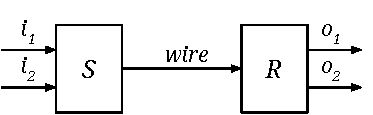
\includegraphics[width=4.2cm]{figures/sender-receiver.pdf}
\vspace{-0.5cm}
\end{wrapfigure}
The sender can send one bit over the wire to the receiver.
We would like to synthesize the sender and receiver modules that satisfy
the following \CTLstar formula over $I = \{i_1,i_2\}$ and $O=\{o_1,o_2\}$:
\begin{align*}
& \AG((i_1 \land i_2)  \impl  \F(o_1  \land  o_2))  \land  \\
& \AG((i_1 \land i_2 \land o_1 \land o_2)  \impl  \X(o_1 \land o_2))  \land  \\
& \AG(~\EF(o_1 \land  \neg o_2)  \land  
       \EF( \neg o_1 \land o_2)  \land  
       \EF( \neg o_1 \land  \neg o_2)  \land  
       \EF(o_1 \land o_2)~).
\end{align*}
Our tool does not support distributed synthesis,
so we manually adapted the SMT query it produced,
by introducing the following uninterpreted functions.
\li
\- For the sender:
   the transition function $\tau_s: T_s \times 2^{\{i_1,i_2\}} \to T_s$
   and the output function $out_s: T_s \times 2^{\{i_1,i_2\}} \to \bbB$.
   We set $T_s$ to have a single state.
\- For the receiver:
   the transition function $\tau_r: T_r \times 2^{\{wire\}} \to T_r$
   and the output functions $o_1: T_r \to \bbB$ and $o_2: T_r \to \bbB$.
   We set $T_r$ to have four states.
\il
It took Z3 solver about 1 minute to find the solution shown in Figure~\ref{fig:sender-receiver}.

\begin{figure}[tb]
\center
\begin{subfigure}[b]{0.45\textwidth}
\begin{tikzpicture}[->,>=stealth',shorten >=1pt,auto,node distance=2cm,semithick]
  \tikzset{every state/.style={minimum size=7mm,inner sep=0.0mm}, initial text={}}
  \tikzstyle{every edge} = [align=center,draw=black]

  \node[state,initial] (0) {$0$};

  \path 
  (0) edge [loop right] node {$wire \equiv \neg i_1\neg i_2$} (0);
\end{tikzpicture}
\caption{The sender (Mealy machine)}
\end{subfigure}
\begin{subfigure}[b]{0.45\textwidth}
\begin{tikzpicture}[->,>=stealth',shorten >=1pt,auto,node distance=2.5cm,semithick]
  \tikzset{every state/.style={minimum size=7mm,inner sep=0.0mm}, initial text={}}
  \tikzstyle{every edge} = [align=center,draw=black]

  \node[state,initial] (0) [label={above:${o_1}\neg{o_2}$}] {$0$};
  \node[state] (3) [right of=0, label={above:$\neg{o_1}{o_2}$}] {$3$};
  \node[state] (1) [below of=3, label={below:${o_1}{o_2}$}] {$1$};
  \node[state] (2) [left of=1, label={below:$\neg{o}_1\neg{o}_2$}] {$2$};

  \path 
  (0) edge node {$\neg{wire}$} (3)
  (0) edge [left] node {$wire$} (2)

  (1) edge [loop right] node {$\neg{wire}$} (1)
  (1) edge [sloped] node {$wire$} (0)

  (2) edge [below] node {$\true$} (1)

  (3) edge node {${wire}$} (1)
  (3) edge [sloped] node {$\neg{wire}$} (2);
\end{tikzpicture}
\caption{The receiver (Moore machine)}
\end{subfigure}
\caption{The synthesized system for the sender-receiver example}
\label{fig:sender-receiver}
\end{figure}


\subsection{Discussion of Bounded Synthesis from \CTLstar}

%In this chapter,
%we showed how the research on ranking functions~\cite{Nir06,jurdzinski2000small}
%can be used to easily derive synthesis procedures.
We described two approaches to the \CTLstar synthesis and
the only (to our knowledge) synthesizer supporting \CTLstar.
(For CTL synthesis see \cite{klenze2016fast,de2012synthesizing,ctlsat},
 and \cite{bounded-pctl} for PCTL.)
The two approaches are conceptually similar.
The approach via direct encoding is easier to code.
The approach via alternating hesitant automata hints,
for example, at how to reduce \CTLstar synthesis to solving safety games:
via
bounding the number of visits to co-B\"uchi final states and
bounding the distance to B\"uchi final states,
and then determinizing the resulting automaton.
A possible future direction is to extend the approach to the logic ATL* and distributed systems.
In the next chapter, we show how \CTLstar synthesis can be reduced to LTL synthesis,
which avoids developing specialized \CTLstar synthesisers,
presented here.


\chapter{\CTLstar Synthesis via LTL Synthesis}\label{chap:ctl-via-ltl}

\hfill {\footnotesize\textit{This chapter is based on joint work with Roderick Bloem and Sven Schewe~\cite{CTLsynt-via-LTLsynt}}.~~~~~~~~}

\begin{quotation}
\noindent\textbf{Abstract.}
We reduce synthesis for \CTLstar properties to synthesis for \LTL.
In the context of model checking this is impossible --- \CTLstar is more expressive than LTL.
Yet, in synthesis we have knowledge of the system structure \emph{and} we can add new outputs.
These outputs can be used to encode witnesses of the satisfaction of \CTLstar subformulas directly into the system.
This way, we construct an LTL formula, over old and new outputs and original inputs,
which is realisable if, and only if, the original \CTLstar formula is realisable.
The \CTLstar-via-LTL synthesis approach preserves the problem complexity,
although it might increase the minimal system size.
We implemented the reduction,
and evaluated the \CTLstar-via-LTL synthesiser on several examples.
\end{quotation}

\iffinal\else
\textcolor{blue}{\small{
TODOs:
\li
\- related work
\- unrealisability section: elaborate on the witness
\il
}
}
\fi


\section{Introduction} \label{sec:intro}

The problem of reactive synthesis was introduced by Church for Monadic Second Order Logic~\cite{Church63}.
Later Pnueli introduced Linear Temporal Logic (LTL)~\cite{pnueli1977temporal}
and together with Rosner proved 2EXPTIME-completeness
of the reactive synthesis problem for LTL~\cite{DBLP:conf/popl/PnueliR89}.
In parallel, Emerson and Clarke introduced Computation Tree Logic (CTL)~\cite{ctl-origin},
and later Emerson and Halpern introduce Computation Tree Star Logic (\CTLstar)~\cite{ctlstar-origin}
that subsumes both CTL and LTL.
Kupferman and Vardi showed~\cite{informatio} that the synthesis problem for \CTLstar is 2EXPTIME-complete.
%The original approach to synthesis from LTL goes via Safra construction~\cite{DBLP:conf/focs/Safra88,DBLP:conf/lics/Piterman06}
%to determinize B\"uchi automata \cite{DBLP:conf/popl/PnueliR89},
%which proved to be hard to implement efficiently.

Intuitively, LTL allows one to reason about infinite computations.
The logic has \emph{temporal} operators, e.g., $\G$ (always) and $\F$ (eventually),
and allows one to state properties like ``every request is eventually granted''
($\G(r \impl \F g)$).
A system satisfies a given LTL property if \emph{all} its computations satisfy it.

In contrast, CTL and \CTLstar reason about computation trees,
usually derived by unfolding the system.
The logics have---in addition to temporal operators---\emph{path quantifiers}:
$\A$ (on all paths) and $\E$ (there exists a path).
CTL forbids arbitrary nesting of path quantifiers and temporal operators:
they must interleave.
E.g.,
$\AG g$ (``on all paths we always grant'') is a CTL formula,
but $\AGF g$ (``on all paths we infinitely often grant'') is not a CTL formula.
\CTLstar lifts this limitation.

The expressive powers of CTL and LTL are incomparable:
there are systems indistinguishable by CTL but distinguishable by LTL, and vice versa.
One important property inexpressible in LTL is the resettability property:
``there is always a way to reach the `reset' state'' ($\AGEF reset$).

% In synthesis,
% \CTLstar also allows the designer to write ``cooperative'' properties,
% that say that a specific behaviour is possible when the environment cooperates,
% yet it leaves open how the environment should cooperate.
% The synthesiser then needs to find a system and the behaviour of the environment
% that together satisfy the property.
% Existentially quantified properties can also be used to ensure that
% the system does not synthesise the specification vacuously, by falsifying the assumptions.

There was a time when CTL and LTL competed for ``best logic for model checking''~\cite{LTL-vs-CTL}.
Nowadays most model checkers use LTL,
because it is easier for designers to think about paths rather than about trees.
LTL is also prevalent in reactive synthesis.
SYNTCOMP~\cite{syntcomp}---the reactive synthesis competition with the goal to popularise reactive synthesis---%
has two distinct tracks, and both use LTL (or variants) as their specification language.

Yet LTL leaves the designer without \emph{structural} properties.
One solution is to develop general \CTLstar synthesisers like the one we developed in Chapter~\ref{chap:bosy:ctlstar}.
Another solution is to transform the \CTLstar synthesis problem into
the form understandable to LTL synthesisers, i.e., to reduce \CTLstar synthesis to LTL synthesis.
Such a reduction would automatically transfer performance advances in LTL synthesisers
to a \CTLstar synthesiser.
In this chapter we show one such reduction.

Our reduction of \CTLstar synthesis to LTL synthesis works as follows.

First, recall how the standard \CTLstar model checking works (see page~\ref{page:defs:bottom-up-mc}).
The verifier introduces a proposition for every state subformula---formulas starting with an $\A$ or an $\E$ path quantifier---of a given \CTLstar formula.
Then the verifier annotates system states with these propositions,
in the bottom up fashion,
starting with propositions that describe subformulas over original propositions (system inputs and outputs).
Therefore the system satisfies the \CTLstar formula iff the initial system state is annotated
with the proposition describing the whole \CTLstar formula
(assuming that the \CTLstar formula starts with $\A$ or $\E$).

Now let us look into \CTLstar synthesis.
The synthesiser has the flexibility to choose the system structure, 
as long as it satisfies a given specification.
We introduce new propositions---outputs that later can be hidden from the user---%
for state subformulas of the \CTLstar formula,
just like in the model checking case above.
We also introduce additional propositions for existentially quantified subformulas---%
to encode the witnesses of their satisfaction.
Such propositions describe the directions (inputs) the environment should provide
to satisfy existentially quantified path formulas.
The requirement that new propositions indeed denote the truth of the subformulas can be stated in LTL.
For example, for a state subformula $\A\varphi$, we introduce proposition $p_{\A\varphi}$,
and require $\G\left[ p_{\A\varphi} \impl \varphi' \right]$,
where $\varphi'$ is $\varphi$ with state subformulas substituted by the propositions.
For an existential subformula $\E\varphi$,
we introduce proposition $p_{\E\varphi}$ and require,
\emph{roughly}, $\G\left[ p_{\E\varphi} \impl ((\G d_{p_{\E\varphi}}) \impl \varphi')\right]$, which states:
if the proposition $p_{\E\varphi}$ holds, then the path along directions encoded by $d_{p_{\E\varphi}}$
satisfies $\varphi'$ (where $\varphi'$ as before).
We wrote ``roughly'', because
there can be several different witnesses for the same existential subformula
starting at different system states:
they may meet in the same system state,
but depart afterwards---then, to be able to depart from the meeting state,
each witness should have its own direction $d$.
We show that, for each existential subformula, a number $\approx 2^{|\Phi_\CTLstar|}$ of witnesses is sufficient,
where $\Phi_\CTLstar$ is a given \CTLstar formula.
This makes the LTL formula exponential in the size of the \CTLstar formula,
but the special---conjunctive---nature of the LTL formula ensures
that the synthesis complexity is 2EXPTIME wrt.\ $|\Phi_\CTLstar|$.

Our reduction is ``if and only if'' and preserves the synthesis complexity.
However, it may increase the size of the system, and is not very well suited to establish unrealisability.
Of course, to show that a given \CTLstar formula is unrealisable,
one could reduce \CTLstar synthesis to LTL synthesis,
then reduce the LTL synthesis problem to solving parity games,
and derive the unrealisability from there%
\footnote{Reducing LTL synthesis to solving parity games \emph{is} practical, as SYNTCOMP'17~\cite{syntcomp} showed:
  such synthesiser {\tt ltlsynt} was among the fastest.}.
But the standard approach for unrealisability checking---by synthesising the dualised LTL specification---does not seem to be practical.
The reason is that the LTL formula $\Phi_\LTL$ is exponential in the size $|\Phi_\CTLstar|$ of the \CTLstar formula.
The negated LTL formula $\neg \Phi$ (used in the dualised specification)
is a big disjunction (vs.\ big conjunction for $\Phi_\LTL$),
which makes a corresponding universal co-B\"uchi automaton doubly-exponential in $|\Phi_\CTLstar|$
(vs.\ singly-exponential for $\Phi_\LTL$).
The double exponential blow up in the size of the automaton---which is used as input to bounded synthesis---%
makes this unrealisability check impractical~\footnote{%
  This is a conjecture:
  we have \emph{not} proven that the synthesis of dualised LTL formulas, produced by our reduction, takes triply exponential time.}%
.

Finally, we have implemented\footnote{Available at \url{https://github.com/5nizza/party-elli}, branch ``cav17''}
the converter from \CTLstar into LTL,
and evaluated our \CTLstar-via-LTL synthesis approach,
using two LTL synthesisers and \CTLstar synthesiser (Chapter~\ref{chap:bosy:ctlstar}),
on several examples.
The experimental results show that such an approach works very well%
---outperforming the specialised \CTLstar synthesiser
   (Chapter~\ref{chap:bosy:ctlstar})---%
when the number of \CTLstar-specific formulas is small.

The chapter depends on notions defined in Chapter~\ref{chap:defs}
and is structured as follows.
In the next Section~\ref{sec:reductions-to-ltl}
we present the main contribution: the reduction.
Then Section~\ref{sec:ctlstar-unreal} briefly discusses checking unrealisability of \CTLstar specifications.
Section~\ref{sec:experiments} describes the experimental setup, specifications, solvers used, and synthesis timings,
and Section~\ref{sec:conclusion} concludes.
\ak{mention related work section}
%Moore systems (Section~\ref{defs:moore-systems}),
%trees (Section~\ref{defs:trees}),
%\CTLstar and LTL (Section~\ref{defs:ctlstar}),
%(can be skipped) hesitant tree automata (Section~\ref{defs:tree-automata}),
%B\"uchi and co-B\"uchi word automata (Section~\ref{defs:word-automata}),
%synthesis problem (Section~\ref{defs:synthesis-problem}).


\section{Converting \CTLstar to \LTL for Synthesis}
\label{sec:reductions-to-ltl}

\ak{
\li
\- unify: LTL vs. path formula
\- system/tree path: sync the def with its usage
\- define det/universal atm that runs on annotated computation trees?
\il
}

In this section, we describe how and why we can reduce \CTLstar synthesis
to LTL synthesis.
First, we recall the standard approach to \CTLstar synthesis,
then describe, step by step, the reduction and the correctness argument,
and then discuss some properties of the reduction.

\subsection{LTL Encoding}

Let us first look at standard automata based algorithms for \CTLstar synthesis~\cite{informatio}\ak{find the approach in their paper}.
%,ScheweThesis}.  \sven{I am not sure if my thesis really belongs there ... .}
When synthesising a system that realizes a \CTLstar specification, we normally do the following.
\li
\- We turn the \CTLstar formula into an alternating hesitant tree automaton $A$.

\- Move from computation trees to annotated computation trees that move the (memoryless) strategy of the verifier%
   \footnote{Such a strategy maps, in each tree node, an automaton state to a next automaton state and direction.}
   into the label of the computation tree.
   This allows for using the derived universal co-B\"uchi tree automaton $U$,
   making the verifier deterministic: it does not make any decisions, as they are now encoded into the system;

\- Determinise $U$ to a deterministic tree automaton $D$.

\- Play an emptiness game for $D$.

\- If the verifier wins, his winning strategy (after projection of the additional labels) defines a system, if the spoiler wins, the specification is unrealisable.
\il

We draw from this construction and use particular properties of the alternating hesitant tree automaton $A$.
Namely, $A$ is not a general alternating tree automaton,
but is an alternating hesitant tree automaton.
Such an automaton is built from a mix of nondeterministic B\"uchi
and universal co-B\"uchi word automata,
called ``existential word automata'' and ``universal word automata''.
These universal and existential word automata start at any system state [tree node] where a universally or existentially, respectively, quantified subformula is marked as true in the annotated system [annotated computation tree].
We use the term ``existential word automata'' to emphasise that the automaton is not only a non-deterministic word automaton, but it is also used in the alternating tree automaton in a way, where the verifier can pick the system [tree] path, along which it has to accept.

We will use the following notions defined on page~\pageref{page:defs:bottom-up-mc}:
the set $F$ of state subformulas of a given \CTLstar formula $\Phi$,
the set of corresponding propositions $P$,
and the top-level Boolean formula $\widetilde\Phi$.

\begin{example}[Word and tree automata]
Consider the formula $\EG\EX(g \land \X(g \land \F\neg g))$
where inputs $I=\{r\}$ and outputs $O=\{g\}$.
The set $F=\{ f_{\EG}=\EG p_{\EX}, f_{\EX}=\EX(g \land \X(g \land \F\neg g)) \}$,
the set $P=\{ p_{\EX}, p_{\EG} \}$, and
$\widetilde\Phi=p_{\EG}$.
Figure~\ref{fig:automata} shows the nondeterministic word automata for the path formulas of the subformulas,
and the alternating (actually, nondeterministic) tree automaton for the whole formula.
In what follows, we work mostly with word automata.

\begin{figure}[tb]
\begin{subfigure}[t]{\linewidth}\center
\begin{tikzpicture}[->,>=stealth',shorten >=1pt,auto,node distance=0.94cm]
  \tikzset{every state/.style={minimum size=3mm,inner sep=0.2mm}, initial text={}}
  \tikzstyle{every edge} = [align=center,draw=black]

  \node[state,initial] (0) {$q_0$};
  \node[state] (1) [right of=0] {$q_1$};
  \node[state] (2) [right of=1] {$q_2$};
  \node[state] (3) [right of=2] {$q_3$};
  \node[state,double] (4) [right of=3] {$q_4$};

  \path
  (0) edge node {$1$} (1)
  (1) edge node {$g$} (2)
  (2) edge node {$g$} (3)
  (3) edge [loop above] node {$g$} (3)
  (3) edge node {$\neg g$} (4)
  (4) edge [loop above] node {$1$} (4);
\end{tikzpicture}
\caption{%
  NBW for $\X (g \land \X (g \land \F\neg g))$,
  the alphabet $\Sigma=2^{\{r,g\}}$.
  Transitions to the non-accepting state $sink$ are not shown.}
\label{fig:nbw-x}
\end{subfigure}
\begin{subfigure}[t]{\linewidth}\center
\begin{tikzpicture}[->,>=stealth',shorten >=1pt,auto,node distance=0.94cm]
  \tikzset{every state/.style={minimum size=3mm,inner sep=0.2mm}, initial text={}}
  \tikzstyle{every edge} = [align=center,draw=black]

  \node[state,initial,double] (0) {$q_0'$};

  \path (0) edge [loop above] node {$p_{\EX}$} (0);
\end{tikzpicture}
\caption{%
  NBW for $\G(p_{\EX})$,
  the alphabet $\Sigma=2^{\{r, g, p_{\EX}\}}$.
  The transition to the non-accepting state $sink$ is omitted.}
\label{fig:nbw-g}
\end{subfigure}
\begin{subfigure}[t]{\linewidth}\center
\begin{tikzpicture}
	\begin{pgfonlayer}{nodelayer}
		\node [style=gn, initial, double] (0) at (0, -0) {$q_0'$};
		\node [style=gn] (1) at (2, -0) {$q_1$};
		\node [style=uptriangle] (2) at (1, -0) {};
		\node [style=gn] (3) at (4, -0) {$q_2$};
		\node [style=gn] (4) at (6, -0) {$q_3$};
		\node [style=gn, double] (5) at (8, -0) {$q_4$};
		\node [style=uptriangle] (6) at (7, -0) {};
		\node [style=uptriangle] (7) at (5, -0) {};
		\node [style=uptriangle] (8) at (3, -0) {};
		\node [style=uptriangle] (9) at (9, -0) {};
		\node [style=uptriangle] (10) at (6, 1) {};
	\end{pgfonlayer}
	\begin{pgfonlayer}{edgelayer}
		\draw [style=simple] (0) to node[below]{$_1$} (2);
		\draw [style=arrow] (2) to node[below=]{$_{\sf E}$} (1);
		\draw [style=arrow, bend right, looseness=1.00] (2) to node[above]{$_{\sf E}$} (0);
		\draw [style=simple] (1) to node[above]{$_g$} (8);
		\draw [style=simple] (3) to node[above]{$_g$} (7);
		\draw [style=simple] (4) to node[above]{$_{\neg g}$} (6);
		\draw [style=simple] (5) to node[below]{$_1$} (9);
		\draw [style=arrow] (8) to node[above]{$_{\sf E}$} (3);
		\draw [style=arrow] (7) to node[above]{$_{\sf E}$} (4);
		\draw [style=arrow] (6) to node[above]{$_{\sf E}$} (5);
		\draw [style=arrow, bend right, looseness=1.00] (9) to node[above]{$_{\sf E}$} (5);
		\draw [style=simple, bend right, looseness=1.00] (4) to node[right]{$_g$} (10);
		\draw [style=arrow, bend right, looseness=1.00] (10) to node[left]{$_{\sf E}$} (4);
	\end{pgfonlayer}
\end{tikzpicture}
\caption{Alternating hesitant tree automaton for $\EG\EX(g \land \X(g \land \F\neg g))$ (actually it is nondeterministic).
  The green color of the states indicate that they are from
  the nondeterministic partition of the states
  (and thus double-circled states are from the B\"uchi acceptance condition).
  The edges starting in the filled triangle are connected with $\land$.
  Edge label $\E$ abbreviates the set of edges, for each tree direction, connected with $\lor$.
  Thus, the transition from $q'_0$ is $((q'_0, r) \lor (q'_0,\neg r)) \land ((q_1, r) \lor (q_1,\neg r))$.
  To get an alternating automaton for $\AG\EX(...)$,
  replace in the self-loop edge of $q_0'$ label $\E$ with $\A$,
  and make the state non-rejecting
  (these also move the state into the universal partition of the states).}
\end{subfigure}
\caption{Word and tree automata.}
\label{fig:automata}
\end{figure}
\end{example}

\smallskip

We are going to show how and why we can reduce \CTLstar-synthesis to LTL synthesis.
The argument is split into steps (a), (b), (c), (d), and (e).
Figure~\ref{fig:discussion-summary} summarises the steps.
\begin{figure}[tbp]
%
\begin{subfigure}{\linewidth}\center
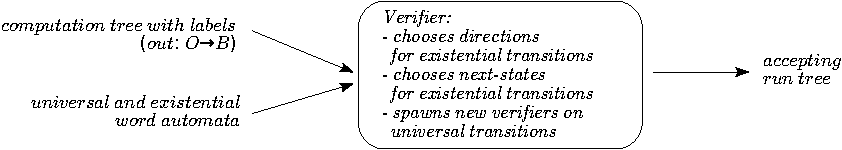
\includegraphics[width=\textwidth]{figures/stepA.pdf}
\caption{The verifier takes a computation tree, universal and existential word automata, and the top-level proposition, that together encode a given \CTLstar formula. It produces an accepting run tree (if the computation tree satisfies the formula).}
\label{fig:stepA}
\end{subfigure}
\vspace{0.1cm}
\hrule
\vspace{0.2cm}
%
\begin{subfigure}{\linewidth}\center
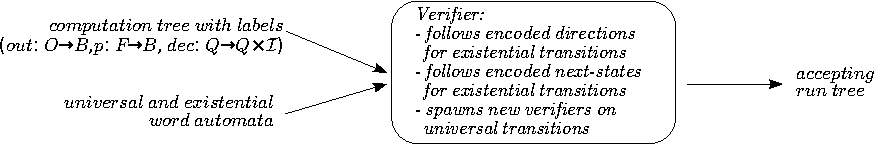
\includegraphics[width=\textwidth]{figures/stepB.pdf}
\caption{We encode the verifier decisions into annotated computation trees,
  making the verifier deterministic.
  Figure~\ref{fig:annotated-computation-tree} shows such an annotated computation tree.}
\label{fig:stepB}
\end{subfigure}
\vspace{0.1cm}
\hrule
\vspace{0.2cm}
%
\begin{subfigure}{\linewidth}\center
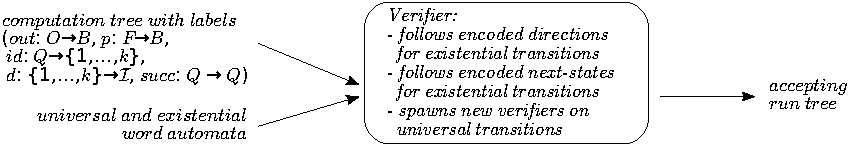
\includegraphics[width=\textwidth]{figures/stepC.pdf}
\caption{The new annotation is a re-phrasing of the previous one.
Figure~\ref{fig:relabeled-tree} gives an example.}
\label{fig:stepC}
\end{subfigure}
\vspace{0.1cm}
\hrule
\vspace{0.2cm}
%
\begin{subfigure}{\linewidth}\center
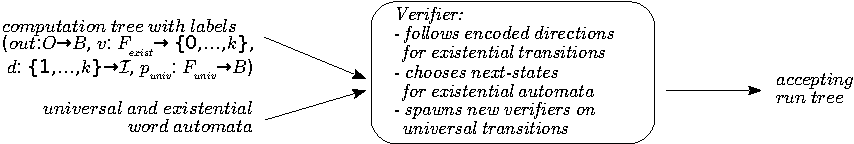
\includegraphics[width=\textwidth]{figures/stepD.pdf}
\caption{We keep directions in the annotation but remove next-states---now the verifier has to choose.
  Figure~\ref{fig:lean-numbered-tree} gives an example.
  The change
  from the label $id: Q \to \{1,...,k\}$
  to the label $v:F_\textit{exist} \to \{0,...,k\}$
  is the reason why the system size can increase.}
\label{fig:stepD}
\end{subfigure}
\vspace{0.1cm}
\hrule
\vspace{0.2cm}
%
\begin{subfigure}{\linewidth}\center
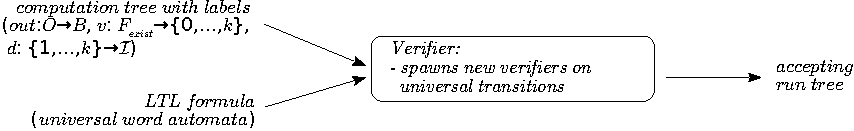
\includegraphics[width=\textwidth]{figures/stepE.pdf}
\caption{Now the obligation of the verifier can be stated in LTL (or using universal co-B\"uchi word automata).}
\label{fig:stepE}
\end{subfigure}
\vspace{0.1cm}
\hrule
\vspace{0.2cm}
%
\caption{Steps in the correctness argument.
  We transform the input to the verifier and its task, step by step.
  We begin with a computation tree labeled with $2^O$
  and end with a computation tree labeled additionally with $v: F_{exist} \to \{0,...,k\}$ and $d:\{1,...,k\} \to \cal I$.
  (Calligraphic $\cal I$ denotes $2^I$.)
  This is about verifying a given computation tree (labels are fixed),
  in synthesis we would search for such a tree.}
\label{fig:discussion-summary}
\end{figure}

\parbf{Step A (the starting point)}
The verifier takes as input:
a computation tree,
universal and existential word automata for the \CTLstar subformulas, and
the top-level proposition corresponding to the whole \CTLstar formula.
It has to produce an accepting run tree
(if the computation tree satisfies the formula).

\parbf{Step B}
Given a computation tree,
the verifier maps each tree node to a (universal or existential word) automaton state,
and moves from a node according to the quantification of the automaton
(either in all tree directions or in one direction).
The decision
in which tree direction to move and which automaton state to pick for the successor node,
constitutes the strategy of the verifier.
Each time the verifier has to move in several tree directions
(this happens when the node is annotated with a \emph{universal} word automaton state),
we spawn a new version of the verifier,
for each tree direction and transition of the universal word automaton.

The strategy of the verifier is a mapping of states of the existential word automata
to a decision,
which consists of a tree direction
(the continuation of the tree path, along which the automaton shall accept)
and an automaton successor state transition.
For every node $n$, this is a mapping
$dec: Q \rightarrow \I \times Q$ \label{page:decision-mapping}
such that $dec(q)=(e,q')$ implies that $q' \in \delta\big(q,(l(n),e)\big)$,
where $\delta$ corresponds to the existential word automaton to which $q$ belongs,
and $l(n) \in \O$ is a label of the current tree node $n$%
\footnote{%
  The verifier, when in the tree node or system state, moves according to this strategy.}%
.
Note that strategies are defined per-node-basis,
i.e., $dec$ may differ in two different nodes $n_1$ and $n_2$.
(All node labels depend on the current node, but we will omit specifying this explicitly.)
Notice that the strategy is memoryless wrt.\ the history of automata states\ak{note why there exists such a strategy}.

We call a model, in which every state is additionally annotated with a verifier strategy, an \emph{annotated model}.
Similarly, an \emph{annotated computation tree} is a computation tree in which every node is additionally annotated with a verifier strategy.
Thus, in both cases, every system state [node] is labeled with:
(i) original propositional labeling $out: O \to \bbB$,
(ii) propositional labeling for universal and existential subformulas $F=F_\textit{univ}\cupdot F_\textit{exist}$, $p: F \to \bbB$, and
(iii) decision labeling $dec: Q \to \I \times Q$ where $Q$ are the states of all existential automata.
\label{page:def:annotated-tree}

\ak{define when an annotated model/tree is accepted}\

\ak{state the relation btw accepted system and accepted annotated system}


\begin{example}
Figure~\ref{fig:annotated-model-tree} shows an annotated system and computation tree.
%
\begin{figure}
\begin{subfigure}[t]{\linewidth}\center
\begin{tikzpicture}
	\begin{pgfonlayer}{nodelayer}
		\node [style=wn, initial below] (0) at (0, -0) {$\bar g$};
		\node [style=wn] (1) at (2, -0) {$g$};
		\node [style=textual] (2) at (-1, -0) {$\color{black}{_{q_0 \mapsto (q_1,r)}}$};
		\node [style=textual] (3) at (-1, -0.25) {$_{q_0' \mapsto (q_0',r)}$};
		\node [style=textual] (4) at (3, -0) {$\color{black}{_{q_0 \mapsto (q_1,r)}}$};
		\node [style=textual] (5) at (3, -0.25) {$_{q_0' \mapsto (q_0',r)}$};
		\node [style=textual] (6) at (-1, 0.25) {$\color{black}{_{q_3 \mapsto (q_4,\bar r)}}$};
		\node [style=textual] (7) at (3, 0.25) {$\color{black}{_{q_1 \mapsto (q_2,r)}}$};
		\node [style=textual] (8) at (3, 0.5) {$\color{black}{_{q_2 \mapsto (q_3,\bar r)}}$};
		\node [style=textual] (9) at (-1, 0.5) {$\color{black}{_{q_4 \mapsto (q_4,\bar r)}}$};
		\node [style=textual] (10) at (3, -0.5) {$_{p_{\sf EX}}$};
		\node [style=textual] (11) at (-1, -0.5) {$_{p_{\sf EX}, p_{\sf EG}}$};
	\end{pgfonlayer}
	\begin{pgfonlayer}{edgelayer}
		\draw [style=arrow, bend right=15, looseness=1.00] (0) to node[below]{$r$} (1);
		\draw [style=arrow, bend right=15, looseness=1.00] (1) to node[above]{$\bar r$} (0);
		\draw [style=arrow, in=120, out=60, loop] (0) to node[below]{$\bar r$} ();
		\draw [style=arrow, in=120, out=60, loop] (1) to node[below]{$r$} ();
	\end{pgfonlayer}
\end{tikzpicture}
\caption{An annotated system satisfying $\EG\EX(g \land \X(g \land \F\neg g))$.
  Near the nodes is the annotation that encodes the winning strategy of the verifier,
  the label $p_{\EX}$ means the subformula $\EX(g \land \X(g \land \F\neg g))$ holds,
  the label $p_{\EG}$ means the subformula $\EG p_{\EX}$ holds.}
\label{fig:annotated-model}
\end{subfigure}

\vspace{0.5cm}
\begin{subfigure}[t]{\linewidth}\center
\center
\begin{tikzpicture}
	\begin{pgfonlayer}{nodelayer}
		\node [style=invisible] (0) at (1, 1) {...};
		\node [initial below, style=wn] (1) at (0, 0.5) {$\bar g$};
		\node [style=wn] (2) at (-2, 1) {$g$};
		\node [style=wn] (3) at (-3, 2) {$g$};
		\node [style=wn] (4) at (-1, 2) {$\bar g$};
		\node [style=wn] (5) at (-0.5, 3) {$\bar g$};
		\node [style=wn] (6) at (-1.5, 3) {$g$};
		\node [style=wn] (7) at (-2.5, 3) {$\bar g$};
		\node [style=wn] (8) at (-3.5, 3) {$g$};
		\node [style=wn] (9) at (-3.75, 4) {$g$};
		\node [style=wn] (10) at (-3.25, 4) {$\bar g$};
		\node [style=wn] (11) at (-2.75, 4) {$g$};
		\node [style=wn] (12) at (-2.25, 4) {$\bar g$};
		\node [style=wn] (13) at (-1.75, 4) {$g$};
		\node [style=wn] (14) at (-1.25, 4) {$\bar g$};
		\node [style=wn] (15) at (-0.75, 4) {$g$};
		\node [style=wn] (16) at (-0.25, 4) {$\bar g$};
		\node [style=textual] (17) at (-0.75, 0.25) {$\color{blue}{_{q_0 \mapsto (q_1,r)}}$};
		\node [style=textual] (18) at (-0.75, -0) {$_{q_0' \mapsto (q_0',r)}$};
		\node [style=textual] (19) at (-2.75, 0.75) {$\color{blue}{_{q_1 \mapsto (q_2,r)}}$};
		\node [style=textual] (20) at (-2.75, 0.5) {$\color{DeepPink}{_{q_0 \mapsto (q_1,r)}}$};
		\node [style=textual] (21) at (-2.75, 0.25) {$_{q_0' \mapsto (q_0',r)}$};
		\node [style=textual] (22) at (-4, 2) {$\color{blue}{_{q_2 \mapsto (q_3,r)}}$};
		\node [style=textual] (23) at (-4, 1.75) {$\color{DeepPink}{_{q_1 \mapsto (q_2,r)}}$};
		\node [style=textual] (24) at (-4, 1.25) {$_{q_0' \mapsto (q_0',r)}$};
		\node [style=textual] (25) at (-4.5, 3.25) {$\color{DeepPink}_{q_2 \mapsto (q_3,\bar r)}$};
		\node [style=textual] (26) at (-4.5, 3.5) {$\color{blue}_{q_3 \mapsto (q_3,\bar r)}$};
		\node [style=textual] (27) at (-4.5, 2.5) {$_{q_0' \mapsto (q_0',r)}$};
		\node [style=textual] (28) at (-4, 1.5) {$\color{Green}{_{q_0 \mapsto (q_1,r)}}$};
		\node [style=textual] (29) at (-4.5, 3) {$\color{Green}_{q_1 \mapsto (q_2,r)}$};
		\node [style=textual] (30) at (-4.5, 2.75) {$\color{DarkGoldenrod}{_{q_0 \mapsto (q_1,r)}}$};
		\node [style=textual] (31) at (-0.75, -0.25) {$_{p_{\sf EX}, p_{\sf EG}}$};
		\node [style=textual] (32) at (-2.75, -0) {$_{p_{\sf EX}}$};
		\node [style=textual] (33) at (-4, 1) {$_{p_{\sf EX}}$};
		\node [style=textual] (34) at (-4.5, 2.25) {$_{p_{\sf EX}}$};
	\end{pgfonlayer}
	\begin{pgfonlayer}{edgelayer}
		\draw [style=arrow] (1) to node{} (0);
		\draw [style=arrow] (4) to (5);
		\draw [style=arrow] (4) to (6);
		\draw [style=arrow] (3) to (7);
		\draw [style=dashed arrow] (3) to (8);
		\draw [style=blue, transform canvas={yshift=0.3mm,xshift=0.8mm}] (3) to (8);
		\draw [style=pink, transform canvas={yshift=0.8mm,xshift=1.4mm}] (3) to (8);
		\draw [style=green, transform canvas={yshift=-0.3mm,xshift=-0.5mm}] (3) to (8);
		\draw [style=dashed arrow, in=-45, out=135, looseness=0.75] (2) to node{} (3);
		\draw [style=blue, transform canvas={yshift=0.7mm,xshift=0.7mm}] (2) to (3);
		\draw [style=pink, transform canvas={yshift=1.3mm,xshift=1.3mm}] (2) to (3);
		\draw [style=arrow] (2) to (4);
		\draw [style=dashed arrow] (1) to node[right]{} (2);
		\draw [style=blue, transform canvas={yshift=0.7mm,xshift=0.1mm}] (1) to (2);
		\draw [style=dashed arrow] (8) to (9);
		\draw [style=green, transform canvas={xshift=-0.5mm,yshift=-0.1mm}] (8) to (9);
		\draw [style=yellow, transform canvas={xshift=-1mm,yshift=-0.2mm}] (8) to (9);
		\draw [style=arrow] (8) to (10);
		\draw [style=blue, transform canvas={xshift=0.5mm,yshift=-0.1mm}] (8) to (10);
		\draw [style=pink, transform canvas={xshift=1mm,yshift=-0.2mm}] (8) to (10);
		\draw [style=arrow] (7) to (11);
		\draw [style=arrow] (7) to (12);
		\draw [style=arrow] (6) to (13);
		\draw [style=arrow] (6) to (14);
		\draw [style=arrow] (5) to (15);
		\draw [style=arrow] (5) to (16);
	\end{pgfonlayer}
\end{tikzpicture}
\caption{%
  An annotated computation tree that satisfies
  $\EG\EX(g \land \X(g \land \F\neg g))$.
  The root node is called $\epsilon$,
  its left child $\mathrm r$, the left child of node $\mathrm r$ is $\mathrm{rr}$, and so on.
  Let $p_{\EG}$ correspond to $\EG(p_{\EX})$
  and let $p_{\EX}$ correspond to $\EX(g \land \X(g \land \F\neg g))$.
  The annotation for the verifier strategy is on the left side of nodes,
  and decisions for non mapped states are irrelevant.
  Paths used by the winning strategy are depicted using dashed and colored lines.
  The black dashed path witnesses $p_{\EG}$,
  the blue path witnesses $p_{\EX}$ starting in the root node $\epsilon$,
  the pink path witnesses $p_{\EX}$ starting in the node $\mathrm r$, and so on.
  The pink and blue paths share the tail.
  Note that this particular annotated computation tree
  is \emph{not} the unfolding of the annotated system above:
  in the annotated system the right state maps $q_2 \mapsto (q_3, \bar r)$,
  while in the tree the node $\mathrm{rr}$ has $q_2 \mapsto (q_3, r)$.
  (This is done to illustrate that mapped out tree paths can share the tail.)
  \ak{put on the right side the atm that eats such trees...and produces acc \emph{run} trees?}}
\label{fig:annotated-computation-tree}
\end{subfigure}
\caption{Annotated system and computation tree.}
\label{fig:annotated-model-tree}
\end{figure}
\end{example}


\parbf{Step C}
\ak{unify: nondet and existential atm}
The verifier strategy (encoded in the annotated computation tree) encodes both
the words on which the nondeterministic automata are interpreted and
witnesses of acceptance
(accepting automata paths on those words).
%that this word is accepted by them.
For the encoding in LTL that we will later use,
it is enough to map out the word,
%(tail of a path through the tree---or its labeling?)
%on which a nondeterministic automaton is interpreted,
and replace the witness by what it actually means:
that the automaton word satisfies the respective path formula.
I.e.,
if a proposition $p$ corresponding to an existential formula $\E \varphi$ holds in a tree node,
then it will be enough to require that $\varphi$ holds
on the path starting in that node and that follows the directions encoded in the tree.

\begin{example}
Let us look at Figure~\ref{fig:annotated-computation-tree}
to understand the notions of mapped out paths and words.
For every proposition marking a tree node there is a mapped out path.
Consider the root node labeled with $p_{\EX}$ and $p_{\EG}$
and look at $p_{\EG}$ first.
The proposition $p_{\EG}$ corresponds to $\EG p_{\EX}$
and is associated with the NBW in Figure~\ref{fig:nbw-g}
that has the initial state $q'_0$.
We consult the strategy $q'_0 \mapsto (q'_0,r)$
and move in direction $r$ into node $\mathrm r$
(note that the root is labeled $p_{\EX}$ and thus we \emph{can} transit $\edge{q'_0}{r}{q'_0}$).
In the node $\mathrm r$ we consult the strategy $q'_0 \mapsto (q'_0,r)$
and again move in direction $r$ into node $\mathrm{rr}$, and so on.
This way we map out the tree path $\epsilon, \mathrm{r}, \mathrm{rr}, ...$
for $p_{\EG}$ from the root,
and the corresponding mapped out word is $(\bar g,p_{\EX},r) (g,p_{\EX},r)^\omega$.
Now consider the root label $p_{\EX}$ that corresponds to $\EX(g \land \X(g \land \F\neg g))$
and is associated with the NBW in Figure~\ref{fig:nbw-x}.
We consult the strategy $q_0 \mapsto (q_1,r)$
that tells us to move in direction $r$ into node $\mathrm{r}$
(again, note that the root label $g$ makes it possible to transit $\edge{q_0}{g}{q_1}$).
In the node $\mathrm r$ we consult the strategy $q_1 \mapsto (q_2,r)$ and move into node $\mathrm{rr}$,
while the automaton state advances to $q_2$.
From the node $\mathrm{rr}$ the strategy $q_2 \mapsto (q_3,r)$ directs us into node $\mathrm{rrr}$,
then the node $\mathrm{rrr}$ has the strategy $q_3 \mapsto (q_3,\bar r)$, and so on.
Thus, from the root for the proposition $p_{\EX}$ the strategy maps out the path
$\epsilon, \mathrm{r}, \mathrm{rr}, \mathrm{rrr}, \mathrm{rr\bar r}, ...$
and the word $(\bar g, r)(g,r)(g,r)(g,\bar r)(\bar g,\bar r)^\omega$.
\end{example}

%Consider the run-tree.
%For every $p$,
%take all infinite paths of the run-tree
%that start in $q_0^p$ and only move in directions $2^I \times Q$.
%Now transform the paths by hiding directions $Q$ (this transforms the nodes, too).
%You will get paths that are mapped out by $p$.
%Union such paths for all $p$.

Let \emph{two tree paths be equivalent} if they share a tail
(equivalently, if one is the tail of the other).
Our interest will be in equivalence of mapped out tree paths.
%To map out the word, we look at the set of tree paths
%--- and here on the tail of the paths, not their labeling ---

There is a simple sufficient condition for two mapped out tree paths to be equivalent:
if they pass through the same node of the annotated computation tree in the same automaton state,
then they have the same future, and are therefore equivalent.
The condition is sufficient but not necessary%
\footnote{%
 Recall that each mapped out tree path corresponds to at least one copy of the verifier that ensures the path is accepting.
 When two verifiers go along the same tree path,
 it can be annotated with different automata states (for example, corresponding to different automata).
 Then such paths do not satisfy the sufficient condition, although they are trivially equivalent.}%
.

\begin{example}
In Figure~\ref{fig:annotated-computation-tree} the blue and pink paths are equivalent,
since they share a tail.
The sufficient condition fires in the node $\mathrm{rrr\bar r}$,
where the tree paths meet in the automaton state $q_3$
%The verifier strategy in that node could be $q_3 \mapsto (q_4,r)$ or $q_3 \mapsto (q_4,\neg r)$.
\end{example}

The sufficient condition implies that we cannot have more non-equivalent tree paths
passing through a tree node than there are states in all existential word automata,
let us call this number $k$:
$k = sum_{\E\varphi \in F_\textit{exist}} |Q_\varphi|$,
where $Q_\varphi$ are the states of an NBW for $\varphi$.
%of existential automata in $A$, call this number $k$.
%Consequently, once we know (or have a lower bound for) this number, say $k$,
For each tree node, we assign unique numbers from $\{1,...,k\}$ to equivalence classes,
and thus any two non-equivalent tree paths that go through the same tree node have different numbers.
As this is an intermediate step in our translation, we are wasteful with the labeling:
\li
\-[(1)] for every node $n$,
        we map existential word automata states to numbers (IDs) using
        $id: Q \to \{1,\ldots,k\}$,
        we also use labels
        $d:\{1,\ldots,k\}\to \I$ (``direction to take'') and
        $succ: Q \to Q$ (``successor to take''),
        such that $succ(q) \in \delta\Big(q, \big(l(n),d(id(q))\big)\Big)$, \emph{and}

\-[(2)] we maintain the same state ID along the chosen direction:\\
        $id_n(q) = id_{n\cdot e}(succ_n(q))$,
        where the subscript denotes a node to which the label belongs
        and $e=d_n(id_n(q))$.
\il

Note that every annotated computation tree can be re-labeled in the above way.
Indeed:
the item (1) alone can be viewed as a re-phrasing of the labeling $dec$ that we had before on page \pageref{page:decision-mapping},
and the requirement (2) is satisfiable because a tree path maintains its equivalence class.
This step is shown in Figure~\ref{fig:stepC}, the labels are:
$(out:O\to\bbB,
p:F\to\bbB,
id: Q \to \{1,\ldots,k\},
d: \{1,\ldots,k\}\to \I,
succ: Q \to Q)$.

Figure~\ref{fig:relabeled-tree} shows a re-labeled computation tree of Figure~\ref{fig:annotated-computation-tree}.
\begin{figure}[tb]
\center
\begin{tikzpicture}
	\begin{pgfonlayer}{nodelayer}
		\node [style=invisible] (0) at (1, 1) {...};
		\node [initial below, style=wn] (1) at (0, 0.5) {$\bar g$};
		\node [style=wn] (2) at (-2, 1) {$g$};
		\node [style=wn] (3) at (-3, 2) {$g$};
		\node [style=wn] (4) at (-1, 2) {$\bar g$};
		\node [style=wn] (5) at (-0.5, 3) {$\bar g$};
		\node [style=wn] (6) at (-1.5, 3) {$g$};
		\node [style=wn] (7) at (-2.5, 3) {$\bar g$};
		\node [style=wn] (8) at (-3.5, 3) {$g$};
		\node [style=wn] (9) at (-3.75, 4) {$g$};
		\node [style=wn] (10) at (-3.25, 4) {$\bar g$};
		\node [style=wn] (11) at (-2.75, 4) {$g$};
		\node [style=wn] (12) at (-2.25, 4) {$\bar g$};
		\node [style=wn] (13) at (-1.75, 4) {$g$};
		\node [style=wn] (14) at (-1.25, 4) {$\bar g$};
		\node [style=wn] (15) at (-0.75, 4) {$g$};
		\node [style=wn] (16) at (-0.25, 4) {$\bar g$};
		\node [style=textual] (17) at (-1, -0) {$\color{blue}{_{q_0 \mapsto (1, q_1), 1 \mapsto r}}$};
		\node [style=textual] (18) at (-3, 0.75) {$\color{blue}{_{q_1 \mapsto (1,q_2), 1 \mapsto r}}$};
		\node [style=textual] (19) at (-3, 0.5) {$\color{DeepPink}{_{q_0 \mapsto (1,q_1)~~~~~}}$};
		\node [style=textual] (20) at (-4.25, 2) {$\color{blue}{_{q_2 \mapsto (1,q_3), 1 \mapsto r}}$};
		\node [style=textual] (21) at (-4.25, 1.75) {$\color{DeepPink}{_{q_1 \mapsto (1,q_2)~~~~~}}$};
		\node [style=textual] (22) at (-4.75, 3.25) {$\color{DeepPink}_{q_2 \mapsto (1,q_3)~~~~~}$};
		\node [style=textual] (23) at (-4.75, 3.5) {$\color{blue}_{q_3 \mapsto (1,q_3), 1 \mapsto \bar r}$};
		\node [style=textual] (24) at (-4.25, 1.5) {$\color{Green}{_{q_0 \mapsto (2,q_1), 2 \mapsto r}}$};
		\node [style=textual] (25) at (-4.75, 3) {$\color{Green}_{q_1 \mapsto (2,q_2), 2 \mapsto r}$};
		\node [style=textual] (26) at (-4.75, 2.75) {$\color{DarkGoldenrod}{_{q_0 \mapsto (3,q_1), 3 \mapsto r}}$};
		\node [style=textual] (27) at (-1, -0.25) {$\color{black}{_{q_0' \mapsto (4, q_0'), 4 \mapsto r}}$};
		\node [style=textual] (28) at (-3, 0.25) {$\color{black}{_{q_0' \mapsto (4, q_0'), 4 \mapsto r}}$};
		\node [style=textual] (29) at (-4.25, 1.25) {$\color{black}{_{q_0' \mapsto (4, q_0'), 4 \mapsto r}}$};
		\node [style=textual] (30) at (-4.75, 2.5) {$\color{black}{_{q_0' \mapsto (4, q_0'), 4 \mapsto r}}$};
		\node [style=textual] (31) at (-1.5, -0.5) {$_{p_{\sf EX}, p_{\sf EG}}$};
		\node [style=textual] (32) at (-3.75, -0) {$_{p_{\sf EX}}$};
		\node [style=textual] (33) at (-5, 1) {$_{p_{\sf EX}}$};
		\node [style=textual] (34) at (-5.5, 2.25) {$_{p_{\sf EX}}$};
	\end{pgfonlayer}
	\begin{pgfonlayer}{edgelayer}
		\draw [style=arrow] (1) to node{} (0);
		\draw [style=arrow] (4) to (5);
		\draw [style=arrow] (4) to (6);
		\draw [style=arrow] (3) to (7);
		\draw [style=dashed arrow] (3) to (8);
		\draw [style=blue, transform canvas={yshift=0.3mm,xshift=0.8mm}] (3) to (8);
		\draw [style=pink, transform canvas={yshift=0.8mm,xshift=1.4mm}] (3) to (8);
		\draw [style=green, transform canvas={yshift=-0.3mm,xshift=-0.5mm}] (3) to (8);
		\draw [style=dashed arrow, in=-45, out=135, looseness=0.75] (2) to node{} (3);
		\draw [style=blue, transform canvas={yshift=0.7mm,xshift=0.7mm}] (2) to (3);
		\draw [style=pink, transform canvas={yshift=1.3mm,xshift=1.3mm}] (2) to (3);
		\draw [style=arrow] (2) to (4);
		\draw [style=dashed arrow] (1) to node[right]{} (2);
		\draw [style=blue, transform canvas={yshift=0.7mm,xshift=0.1mm}] (1) to (2);
		\draw [style=dashed arrow] (8) to (9);
		\draw [style=green, transform canvas={xshift=-0.5mm,yshift=-0.1mm}] (8) to (9);
		\draw [style=yellow, transform canvas={xshift=-1mm,yshift=-0.2mm}] (8) to (9);
		\draw [style=arrow] (8) to (10);
		\draw [style=blue, transform canvas={xshift=0.5mm,yshift=-0.1mm}] (8) to (10);
		\draw [style=pink, transform canvas={xshift=1mm,yshift=-0.2mm}] (8) to (10);
		\draw [style=arrow] (7) to (11);
		\draw [style=arrow] (7) to (12);
		\draw [style=arrow] (6) to (13);
		\draw [style=arrow] (6) to (14);
		\draw [style=arrow] (5) to (15);
		\draw [style=arrow] (5) to (16);
	\end{pgfonlayer}
\end{tikzpicture}
\caption{%
  A re-labeled computation tree.
  Notation ``$q_0 \mapsto (1,q_1)$'' means
  $id(q_0) = 1$ and $succ(q_0) = q_1$, and ``$1 \mapsto r$'' means $d$ maps $1$ to $\{r\}$.
  Since the blue and pink paths are equivalent,
  the label $id$ maps the corresponding automata states in the nodes
  to the same number, $1$.
  The IDs of the green and yellow paths differ implying that they are not equivalent and hence do not share the tail (their tails cannot be seen in the figure).
}
\label{fig:relabeled-tree}
\end{figure}

\parbf{Step D}
In the new annotation with labels $(out, p, id, d, succ)$,
labeling $d$ alone maps out the tree path for each ID.
The remainder of the information is mainly there to establish that the corresponding word\ak{which alphabet?}
is accepted by the respective word automaton (equivalently: satisfies the respective path formula).
%---or, likewise, that the corresponding word satisfies the respective path formula.
If we use only $d$, then the only missing information is where the path starts and which path formula it belongs to---the information originally encoded by $p$.

%We address these two points by providing this information through changing from rich to numbered computation trees: where the rich computation trees have a \emph{propositional} label for each existentially quantified path formula, we replace this propositional label by an \emph{ID}, where $0$ encodes that no claim that this subformula holds is made (similar to a proposition being ``false'' in the rich model), whereas an ID between $1$ and $k$ is interpreted like a ``true'' flag, but also requires that a respective witness is marked out with the given ID.

We address these two points by using \emph{numbered} computation trees.
Recall that the annotated computation trees have a \emph{propositional} labeling
$p: F \to \bbB$ that labels nodes with subformulas.
In the numbered computation trees,
we replace $p$ for \emph{existential} subformulas $F_\textit{exist} \subseteq F$
by labeling ${v: F_\textit{exist} \to \{0,...,k\}}$,
where for every existentially quantified formula $\E\varphi \in F_\textit{exist}$ and a tree node $n$:
\li
\- $v_{\E\varphi,n}=0$ encodes that no claim that $\E\varphi$ holds in $n$ is made
   (similarly to the proposition $p_{\E\varphi}$ being false in the annotated tree), whereas

\- a value $v_{\E\varphi,n} \in \{1,...,k\}$
   requires that the word of a tree path with ID $v_{\E\varphi,n}$
   starting in $n$ and that follows $d(v_{\E\varphi,n})$ satisfies $\varphi$,
   i.e.,
   the word corresponding to
   $n,
   n\!\cdot\! d_n(v_{\E\varphi,n}),
   n\!\cdot\! d_n(v_{\E\varphi,n}) \!\cdot\! d_{n\!\cdot\! d_n(v_{\E\varphi,n})}(v_{\E\varphi,n}),...$
   satisfies $\varphi$
   (where $d_n$ denotes $d$ in node $n$).
\il
% ak: "similarly" means that the verifier consults the direction-successor for the corresponding q0
% ak: "similarly" uses the fact that in in the annotated trees
% having a node marked with a subformula means that
% the node witnesses the subformula with the marked out path
% (the path is marked out by the strategy and we start in atm state q0)
% For A\phi subformulas, all paths must satisfy \phi---this is ensured
% by the verifier
% (that ensures that all such paths are accepted by the automaton).

\begin{example}
The tree in Figure~\ref{fig:relabeled-tree} becomes a numbered computation tree
if we replace the propositional labels $p_{\EX}$ and $p_{\EG}$ with ID numbers as follows.
The root $\epsilon$ has $v_{\EX} = 1$ and $v_{\EG} = 4$,
the left child $\mathrm r$ has $v_{\EX} = 1$,
the node $\mathrm{rr}$ has $v_{\EX} = 2$,
the node $\mathrm{rrr}$ has $v_{\EX} = 3$.
Note that $id(q_0) = v_{\EX}$ and $id(q_0') = v_{\EG}$ whenever those $v$s are non-zero.
The nodes outside of the dashed path have $v_{\EX} = v_{\EG} = 0$,
meaning that no claims about satisfaction of the corresponding path formulas is made.
\end{example}

Initially, we use \emph{ID} labeling $v$ in addition with ($out, id, d, succ, p^\textit{univ}$),
where $p^\textit{univ}$ is a restriction of $p$ on $F_\textit{univ}$,
and then there is no relevant change in the way the (deterministic) verifier works.
I.e., a numbered computation tree can be turned into annotated computation tree, and vice versa,
such that the numbered tree is accepted iff the annotated tree is accepted.
% The direction rich $\leftarrow$ numbered is easy,
% the direction rich $\rightarrow$ numbered could be better formalized (?): it follows from the fact the number of equivalence classes passing through a node is less or equal to $k$.
%(Indeed: it suffices that an initial state of the respective existential word automaton is in the pre-image of ID for $id$ whenever ID is not $0$.)

\begin{figure}[tb]
\center
\begin{tikzpicture}
	\begin{pgfonlayer}{nodelayer}
		\node [style=invisible] (0) at (1, 1) {...};
		\node [style=wn, initial below] (1) at (0, 0.5) {$\bar g$};
		\node [style=wn] (2) at (-2, 1) {$g$};
		\node [style=wn] (3) at (-3, 2) {$g$};
		\node [style=wn] (4) at (-1, 2) {$\bar g$};
		\node [style=wn] (5) at (-0.5, 3) {$\bar g$};
		\node [style=wn] (6) at (-1.5, 3) {$g$};
		\node [style=wn] (7) at (-2.5, 3) {$\bar g$};
		\node [style=wn] (8) at (-3.5, 3) {$g$};
		\node [style=wn] (9) at (-3.75, 4) {$g$};
		\node [style=wn] (10) at (-3.25, 4) {$\bar g$};
		\node [style=wn] (11) at (-2.75, 4) {$g$};
		\node [style=wn] (12) at (-2.25, 4) {$\bar g$};
		\node [style=wn] (13) at (-1.75, 4) {$g$};
		\node [style=wn] (14) at (-1.25, 4) {$\bar g$};
		\node [style=wn] (15) at (-0.75, 4) {$g$};
		\node [style=wn] (16) at (-0.25, 4) {$\bar g$};
		\node [style=textual] (17) at (-0.75, 0.25) {$\color{black}{_{1 \mapsto r}}$};
		\node [style=textual] (18) at (-0.75, -0) {$\color{black}{_{4 \mapsto r}}$};
		\node [style=textual] (19) at (-0.75, -0.25) {$_{{\color{blue}{v_{\sf EX}=1}}, v_{\sf EG}=4}$};
		\node [style=textual] (20) at (-2.75, 0.5) {$\color{black}{_{4 \mapsto r}}$};
		\node [style=textual] (21) at (-2.75, 0.75) {$\color{black}{_{1 \mapsto r}}$};
		\node [style=textual] (22) at (-2.75, 0.25) {$_{{\color{DeepPink}{v_{\sf EX}=1}}}$};
		\node [style=textual] (23) at (-3.75, 1.5) {$\color{black}{_{4 \mapsto r}}$};
		\node [style=textual] (24) at (-3.75, 1.25) {$_{{\color{Green}{v_{\sf EX}=2}}}$};
		\node [style=textual] (25) at (-3.75, 2) {$\color{black}{_{1 \mapsto r}}$};
		\node [style=textual] (26) at (-3.75, 1.75) {$\color{black}{_{2 \mapsto r}}$};
		\node [style=textual] (27) at (-4.25, 2.75) {$\color{black}{_{4 \mapsto r}}$};
		\node [style=textual] (28) at (-4.25, 2.5) {$_{{\color{DarkGoldenrod}{v_{\sf EX}=3}}}$};
		\node [style=textual] (29) at (-4.25, 3.5) {$\color{black}{_{1 \mapsto \bar r}}$};
		\node [style=textual] (30) at (-4.25, 3.25) {$\color{black}{_{2 \mapsto r}}$};
		\node [style=textual] (31) at (-4.25, 3) {$\color{black}{_{3 \mapsto r}}$};
	\end{pgfonlayer}
	\begin{pgfonlayer}{edgelayer}
		\draw [style=arrow] (1) to node{} (0);
		\draw [style=arrow] (4) to (5);
		\draw [style=arrow] (4) to (6);
		\draw [style=arrow] (3) to (7);
		\draw [style=dashed arrow] (3) to (8);
		\draw [transform canvas={yshift=0.3mm,xshift=0.8mm}, style=blue] (3) to (8);
		\draw [transform canvas={yshift=0.8mm,xshift=1.4mm}, style=pink] (3) to (8);
		\draw [transform canvas={yshift=-0.3mm,xshift=-0.5mm}, style=green] (3) to (8);
		\draw [style=dashed arrow, in=-45, out=135, looseness=0.75] (2) to node{} (3);
		\draw [transform canvas={yshift=0.7mm,xshift=0.7mm}, style=blue] (2) to (3);
		\draw [transform canvas={yshift=1.3mm,xshift=1.3mm}, style=pink] (2) to (3);
		\draw [style=arrow] (2) to (4);
		\draw [style=dashed arrow] (1) to node[right]{} (2);
		\draw [transform canvas={yshift=0.7mm,xshift=0.1mm}, style=blue] (1) to (2);
		\draw [style=dashed arrow] (8) to (9);
		\draw [transform canvas={xshift=-0.5mm,yshift=-0.1mm}, style=green] (8) to (9);
		\draw [transform canvas={xshift=-1mm,yshift=-0.2mm}, style=yellow] (8) to (9);
		\draw [style=arrow] (8) to (10);
		\draw [transform canvas={xshift=0.5mm,yshift=-0.1mm}, style=blue] (8) to (10);
		\draw [transform canvas={xshift=1mm,yshift=-0.2mm}, style=pink] (8) to (10);
		\draw [style=arrow] (7) to (11);
		\draw [style=arrow] (7) to (12);
		\draw [style=arrow] (6) to (13);
		\draw [style=arrow] (6) to (14);
		\draw [style=arrow] (5) to (15);
		\draw [style=arrow] (5) to (16);
	\end{pgfonlayer}
\end{tikzpicture}
\caption{%
  Numbered computation tree with redundant annotations removed.}
\label{fig:lean-numbered-tree}
\end{figure}

\ak{define 'tree path satisfies LTL', remove 'word' in many places}

Now we observe that the labelings $id$ and $succ$
are used only to witness that each word mapped out by $d$
is accepted by respective existential word automata.
I.e., $id$ and $succ$ make the verifier deterministic.
Let us remove $id$ and $succ$ from the labeling.
We call such trees \emph{lean-numbered computation trees};
they have labeling
$
(
out:O \to \bbB, 
v:F_\textit{exist} \to \{0,...,k\},
d:\{1,...,k\} \to \I,
p^\textit{univ}: F_\textit{univ} \to \bbB
)
$.
This makes the verifier nondeterministic.
We still have the property that
every accepting annotated computation tree can be turned into
an accepting lean-numbered computation tree,
and vice versa.
This step is shown in Figure~\ref{fig:stepD};
an example of a lean-numbered computation tree is in Figure~\ref{fig:lean-numbered-tree}.

\parbf{Step E (the final step)}
We show how labeling $(out,v,d,p^\textit{univ})$ 
allows for using LTL formulas instead of directly using automata for the acceptance check.
The encoding into LTL is as follows.
\li
\- For each existentially quantified formula $\E\varphi$,
   we introduce the following LTL formula
   (recall that $v_{\E\varphi} = 0$ encodes that we do \emph{not} claim that $\E\varphi$ holds in the current     tree node,
    and $v_{\E\varphi} \neq 0$ means that $\E\varphi$ does hold
    and $\varphi$ holds if we follow $v_{\E\varphi}$-numbered directions):
   \begin{equation}\label{eq:ltl-existential}
   \bigwedge_{j \in \{1,...,k\}} \G\Big[ v_{\E\varphi} = j ~\impl~ \big( \G d_j \impl \varphi'\big) \Big],
   \end{equation}
   where $\varphi'$ is obtained from $\varphi$
   by replacing the subformulas of the form $\E\psi$ by $v_{\E\psi} \neq 0$
   and the subformulas of the form $\A\psi$ by $p_{\A\psi}$.

\- For each subformula of the form $\A\varphi$, we simply take
   \begin{equation}\label{eq:ltl-universal}
   \G\Big[ p_{\A\varphi} ~\impl~ \varphi' \Big],
   \end{equation}
   where $\varphi'$ is obtained from $\varphi$ as before.

\- Finally, the overall LTL formula is the conjunction
   \begin{equation}\label{eq:ltl-full}
   \boxed{
   \Phi' \land \bigwedge_{\E\varphi \in F_\textit{exist}} \text{Eq.}\ref{eq:ltl-existential} ~\land \bigwedge_{\A\varphi \in F_\textit{univ}} \text{Eq.}\ref{eq:ltl-universal}
   }
   \end{equation}
   where the Boolean formula $\Phi'$ is obtained by replacing in the original \CTLstar formula
   every $\E\varphi$ by $v_{\E\varphi} \neq 0$ and every $\A\varphi$ by $p_{\A\varphi}$.
\il

\begin{example}\label{ex:ctlstar}
Let $I = \{r\}$, $O=\{g\}$.
Consider the \CTL formula
$$
\EG \neg g \land \AG\EF \neg g \land \EF g.
$$
The sum of states of individual NBWs is $5$
(assuming the natural translations),
so we introduce integer propositions $v_{\EF\!\bar{g}}$, $v_{\EG\!\bar{g}}$, $v_{\EF\!g}$, ranging over $\{0,...,5\}$,
%\footnote{%
%  We can slightly optimize the LTL formula by using smaller domains for $v_i$s:
%  each $v_i$ can vary over \hl{xx:non-intersecting}
%  where $Q_i$ is the number of states in the corresponding NBW.
%  }
and five Boolean propositions $d_1$, ..., $d_5$;
we also introduce the Boolean proposition $p_{\AG(v_{\EF\!\bar{g}}\neq 0)}$.
The LTL formula is:
\begin{align*}
&~~~v_{\EG\!\bar{g}} \neq 0 \land p_{\AG(v_{\EF\!\bar{g}}\neq 0)} \land v_{\EF\!g} \neq 0 ~\land \\
&\bigwedge_{j \in \{1...5\}}\G \left[
\begin{aligned}
& v_{\EF\!\bar{g}}=j ~\impl~ (\G d_j \impl \F \neg g) \\
& v_{\EG\!\bar{g}}=j ~\impl~ (\G d_j \impl \G \neg g) \\
& v_{\EF\!g}=j ~\impl~ (\G d_j \impl \F g)
\end{aligned}
\right] ~\land\\
&~~~\G\left[p_{\AG(v_{\EF\!\bar{g}}\neq 0)} \impl \G(v_{\EF\!\bar{g}}\neq 0)\right].
\end{align*}
Figure~\ref{fig:ctlstar:system} shows a system satisfying the LTL specification.

\begin{figure}[bt]
\center
\begin{tikzpicture}[->,>=stealth',shorten >=1pt,auto,node distance=3.2cm]
  \tikzset{every state/.style={minimum size=6mm,inner sep=0.0mm}, initial text={}}
  \tikzstyle{every edge} = [align=center,draw=black]

  \node[state,initial below] (0)
  [label={left:\specialcellC{$p_{\AG(v_{\EF\bar g}\neq 0)}$\\$v_{\EF\!\bar{g}}=v_{\EG\!\bar{g}}=2,d_2=\neg r$\\$v_{\EF\!g}=3, d_3=r$}},
   label={below right:$t_0$}] {$\neg g$};
  \node[state] (1)
  [right of=0,
  label={right:\specialcellL{$v_{\EF\!\bar{g}}=2,d_2=r$\\$v_{\EG\!\bar{g}}=v_{\EF\!g}=0$}},
  label={below left:$t_1$}] {$g$};

  \path
  (0) edge [bend left=10] node {$r$} (1)
  (1) edge [bend left=10] node {$r$} (0)
  (1) edge [loop above] node {$\neg r$} (1)
  (0) edge [loop above] node {$\neg r$} (0);
\end{tikzpicture}
\caption{A Moore machine for Example~\ref{ex:ctlstar}.
The witness for $\EG\neg g$ is:
$v_{\EG\!\bar{g}}(t_0)=2$, we move along $d_2=\neg r$ looping in $t_0$, thus the witness is $(t_0)^\omega$.
The witness for $\EF g$:
since $v_{\EF\!g}(t_0)=3$, we move along $d_3=r$ from $t_0$ to $t_1$,
where $d_3$ is not restricted, so let $d_3=\neg r$ (not drawn) and then the witness is $t_0 (t_1)^\omega$.
The satisfaction of $\AGEF \neg g$ means that every state has $v_{\EF\!\bar{g}} \neq 0$, which is true.
In $t_0$ we have $\neg g$, so $\EF \neg g$ is satisfied;
for $t_1$ we have $v_{\EF\!\bar{g}}(t_1)=2$ hence we move $t_1 \trans{r} t_0$ and $\EF \neg g$ is also satisfied.
}
\label{fig:ctlstar:system}
\end{figure}
\end{example}

\begin{remark}[We \emph{need} propositions for universal subformulas]
It is intuitively clear that we need new propositions for existential subformulas.
But it is tempting to believe that we can skip introducing new propositions for universal subformulas
and directly use the subformulas instead of the propositions.
This is wrong.
Consider the \CTLstar formula $\AFAG g$.
Our reduction produces the LTL formula
$$
p_{\AF} \land \G [p_{\AF} \impl \F p_{\AG}] \land \G [p_{\AG} \impl \G g].
$$
If we substitute the new propositions with what they express ($p_{\AF}$ by $\F p_{\AG}$ and $p_{\AG}$ by $\G g$),
then we get $\FG g$.
But $\AFAG g$ is different from $\AFG g$.
\end{remark}

%So far we have talked about computation trees.
%Finally, note that, whenever there is a computation tree satisfying an LTL formula,
%there is a finite system satisfying it~\cite{LTL-finite-model-property}.
\ak{restore this note}

\smallskip

The whole discussion leads us to the theorem.
\begin{theorem}
  Let $I$ be the set of inputs and $O$ be the set of outputs,
  and $\Phi_\LTL$ be derived from a given $\Phi_\CTLstar$ as described above.
  Then:
  $$
  \textit{
  $\Phi_\CTLstar$ is realisable
  $~\Iff~$
  $\Phi_\LTL$ is realisable.
  }
  $$
\end{theorem}


\subsection{Complexity}
The translated LTL formula $\Phi_\text{LTL}$, due to Eq.~\ref{eq:ltl-existential},
in the worst case, can be exponentially larger than $\Phi_\CTLstar$,
$|\Phi_\LTL| = 2^{\Theta(|\Phi_\CTLstar|)}$.
Yet, the upper bound on the size of $UCW_{\Phi_\LTL}$ is $2^{\Theta(|\Phi_\CTLstar|)}$
rather than $2^{\Theta(|\Phi_\LTL|)}=2^{2^{\Theta(|\Phi_\CTLstar|)}}$,
because:
\li
\- the size of the UCW is additive in the size of the UCWs of the individual conjuncts, and
\- each conjunct UCW has almost the same size as a UCW of the corresponding subformula,
   since, for every LTL formula $\varphi$, $|UCW_{\G[p \impl (\G\!d \impl \varphi)]}| = |UCW_\varphi|+1$.%
   \footnote{To see this, recall that we can get $UCW_\psi$ by
     treating $NBW_{\neg\psi}$ as a UCW,
     and notice that $|NBW_{\F[p\land\G\!d\land\neg\varphi]}| = |NBW_{\neg\varphi}|+1$.}
\il
Determinising $UCW_{\Phi_\LTL}$ gives a parity game with up to $2^{2^{\Theta(|\Phi_\CTLstar|)}}$ states and
$2^{\Theta(|\Phi_\CTLstar|)}$ priorities~\cite{Schewe/09/determinise,Piterman07,Safra}.
The recent quasipolynomial algorithm~\cite{DBLP:conf/stoc/CaludeJKL017} for solving parity games
has a particular case for $n$ states and $log(n)$ many priorities,
where the time cost is polynomial in the number of game states.
This gives us $O(2^{2^{|\Phi_\CTLstar|}})$-time solution to the derived LTL synthesis problem.
The lower bound comes from the 2EXPTIME-completeness of the \CTLstar synthesis problem~\cite{RosnerThesis}.


\begin{theorem}
  Our solution to the \CTLstar synthesis problem
  via the reduction to \LTL synthesis
  is 2EXPTIME-complete.
\end{theorem}

\subsection*{Minimality}
Although the reduction to LTL synthesis preserves the complexity class,
it does not preserve the minimality of the systems.
Consider an existentially quantified formula $\E\varphi$.
A system path satisfying the formula may pass through the same system state more than once
and exit it in different directions.%
  \footnote{%
  E.g., in Figure~\ref{fig:annotated-model} the system path $t_0 t_1 t_1 (t_0)^\omega$,
  satisfying $\EX(g\land\X(g\land\F\neg g))$,
  double-visits state $t_1$ and exits it first in direction $r$ and then in $\neg r$,
  where $t_0$ is the system state on the left and $t_1$ is on the right.}
Our encoding forbids that.%
  \footnote{%
  Recall that with $\E\varphi$ we associate a number $v_{\E\varphi}$,
  such that whenever in a system state $v_{\E\varphi}$ is non-zero,
  then the path mapped out by $v_{\E\varphi}$-numbered directions satisfies the path formula $\varphi$.
  Therefore whenever $v_{\E\varphi}$-numbered path visits a system state,
  it exits it in the \emph{same} direction $d_{v_{\E\varphi}}$.
  %I.e., a $v_{\E\varphi}$-numbered path can visit a \ul{system state}
  %zero times, once, or infinitely many times.
  %I.e., any $v_{\E\varphi}$-numbered path is a simple lasso.
  }
I.e., in any system satisfying the derived LTL formula,
a system path mapped out by an ID has a unique outgoing direction from every visited state.
As a consequence, such systems are less concise.\ak{what is the worst case blowup?}
This is illustrated in the following example.

\begin{example}[Non-minimality]\label{ex:ctlstar:nonminimal}
Let $I = \{r\}$, $O=\{g\}$,
and consider the \CTLstar formula
$$
\EX(g \land \X(g \land \F\neg g))
$$
The NBW automaton for the path formula has 5 states (Figure~\ref{fig:nbw-x}),
so we introduce the integer proposition $v$ ranging over $\{0,...,5\}$
and Boolean propositions $d_1$, $d_2$, $d_3$, $d_4$, $d_5$.
The LTL formula is
$$
~~~v \neq 0 ~\land
\bigwedge_{j \in \{1...5\}}\!\!\!\!
\G\big[v=j ~\impl~ (\G d_j \impl \X(g \land \X(g \land \F\neg g)))\big]
$$
A smallest system for this LTL formula is in Figure~\ref{fig:ctlstar:nonminimal:system:ltl}.
It is of size is $3$,
while a smallest system for the original \CTLstar formula is of size $2$
(Figure~\ref{fig:annotated-model}).
\begin{figure}[tb]\center
\begin{tikzpicture}[->,>=stealth',shorten >=1pt,auto,node distance=2.2cm]
  \tikzset{every state/.style={minimum size=6mm,inner sep=0.0mm}, initial text={}}
  \tikzstyle{every edge} = [align=center,draw=black]

  \node[state,initial] (0)
  [label={above right:\specialcellC{$v=1$\\$d_1=\neg r$}},
   label={below:$t_0$}] {$\neg g$};

  \node[state] (1)
  [right of=0,
  label={right:{$d_1=r$}},
  label={below left:$t_1$}] {$g$};

  \node[state] (2)
  [below of=1,
  label=left:{$t_2$},
  label=right:{$d_1=r$}
  ] {$g$};

  \path
  (0) edge node[below] {$\neg r$} (1)
  (1) edge [loop above] node {$\neg r$} (1)
  (1) edge node {$r$} (2)
  (2) edge node {$1$} (0)
  (0) edge [loop above] node {$r$} (0);
\end{tikzpicture}
\caption{%
  A smallest Moore machine satisfying the LTL formula from Example~\ref{ex:ctlstar:nonminimal}.}
\label{fig:ctlstar:nonminimal:system:ltl}
\end{figure}
\end{example}


\subsection{Bounded Reduction}

While we have realisability equivalence for sufficiently large $k$, $k$ is a parameter,
where much smaller $k$ might suffice.
In the spirit of Bounded Synthesis,
it is possible to use smaller parameters in the hope of finding a system.
These systems might be of interest in that they guarantee a limited entanglement of different mapped out paths,
as they cap the number of such paths that can go through the same node of a tree.
Such systems are therefore simple wrt.\ this metric,
and this metric is independent of the automaton representation.
(As opposed to a lower bound for $k$
 that depends on the existential automata.)

\ak{CTL?}
%\input{ctl-encoding}



\section{Checking Unrealisability of \CTLstar} \label{sec:ctlstar-unreal}

What does a witness of unrealisability for \CTLstar look like?
I.e., when a formula is unrealisable,
is there an ``environment model'', like in the LTL case,
which disproves any system model?

The LTL formula and the annotation shed light on this:
the system for the dualised case is a strategy how to choose original inputs
(depending on the history of $v$, $d$, $p$, and original outputs),
such that any path in the resulting tree violates the original LTL formula.
I.e., the spoiler strategy is a tree, whose nodes are labeled with original inputs,
and whose directions are defined by $v$, $d$, $p$, and original outputs.

% The spoiler would prefer to annotate tree nodes in conformance with some direction $d$
% and to satisfy $\neg\varphi'$
% in Eq.~\ref{eq:ltl-existential} or Eq.~\ref{eq:ltl-universal},
% whenever the implications are triggered.
% I.e. the spoiler has a current direction to follow,
% as well as a set of ``promising'' directions,

\begin{example}
Consider an unrealisable \CTLstar specification:
$\AG g \land \EFX\neg g$ with inputs $\{r\}$ and outputs $\{g\}$.
After reduction to LTL we get the specification:
inputs $\{r\}$, outputs $\{g,p_{\AG\!g},v_{\EFX\!\bar g},d_1,d_2\}$,
and the LTL formula
$$
p_{\AG\!g} \land v_{\EFX\!\bar g} \neq 0 \land
\G\big[ p_{\AG\!g} \impl \G g \big] \land\!\!\!
\bigwedge_{j \in \{1,2\}}\!\!\!\!\!\G\big[ (v_{\EFX\!\bar g} = j \land \G d_j)  \impl  \F\!\X\neg g \big].
$$
The dual specification is:
the system type is Mealy,
new inputs $\{g,p_{\AG\!g},v_{\EFX\!\bar g},d_1,d_2\}$,
new outputs $\{r\}$,
and the LTL formula is the negated original LTL:
$$
p_{\AG\!g} \land v_{\EFX\!\bar g} \neq 0 \land
\G\big[ p_{\AG\!g} \impl \G g \big] ~\impl\!
\bigvee_{j \in \{1,2\}}\!\!\!\!\!\F\big[ (v_{\EFX\!\bar g} = j \land \G d_j)  \land  \G\!\X g \big].
$$
This dual specification is realisable, and it exhibits, e.g., the following witness of unrealisability:
the output $r$ follows $d_1$ or $d_2$ depending on input $v_{\EFX\!\bar g}$.
(The new system needs two states.
 State $1$ describes ``I've seen $v_{\EFX\!\bar g}\in\{0,1\}$ and I output $r$ equal to  $d_1$'';
 from state $1$ we irrevocably go into state $2$ once $v_{\EFX\!\bar g}=2$ and make $r$ equal to $d_2$).
\end{example}

Although our encoding allows for checking unrealisability of \CTLstar
(via dualising the converted LTL specification),
this approach suffers from a very high complexity.
Recall that the LTL formula can become exponential in the size of a \CTLstar formula,
which could only be handled
because it became a big conjunction with sufficiently small conjuncts.
After negating it becomes a large disjunction,
which makes the corresponding UCW doubly exponential in the size of the initial \CTLstar specification
(vs.\ single exponential for the non-negated case).
%Not only can $k$ be exponential in the size of the $\CTLstar$ formula making the LTL formula exponential,
%all is multiplicative here. % we cannot seem to bound the game size by 2EXP (3EXP --- yes)
This seems---there may be a more clever analysis of the formula structure---%
to make the unrealisability check via reduction to LTL cost three exponents in the worst case
(vs.\ 2EXP by the standard approach).

What one could try is to let the new system player in the dualised game
choose a number of disjunctive formulas to follow,
and allow it to revoke the choice finitely many times.\ak{clarify}
This is conservative:
if following $m$ different disjuncts in the dualised formula is enough to win,
then the new system wins.
% There does not seem to be good complexity guarantees that go with this,
% but with a bit of luck that might work.

Alternatively, one could try to synthesise environment model for parts of the disjunction
increasing them until all disjunctions are used.
This is precise.

\ak{
\hl{%
  Is there a bounded procedure which is like $2^{2^{|\Phi_\CTLstar|}\cdot 2^{\textit{smallest size}}}$
  where the 2exp is in the SMT solver? (just like in the bounded synthesis?)}
}



\section{Experiments}\label{sec:experiments}

We implemented the \CTLstar to LTL converter {\small\tt ctl\_to\_ltl.py} inside PARTY~\cite{party}.
PARTY also has two implementations of Bounded Synthesis~\cite{BS},
one encodes the problem into SMT and another reduces the problem to safety games.
Also, PARTY has a \CTLstar synthesiser based on Bounded Synthesis idea
that encodes the problem into SMT (presented in Chapter~\ref{chap:bosy:ctlstar}).
In this section we compare those three solvers,
where the first two solvers take LTL formulas produced by our converter.
All logs and the code are available in repository {\small\url{https://github.com/5nizza/party-elli}},
the branch ``cav17''.

%The results are in Table~\ref{tab:optimizations}, let us analyse them.


\parbf{Specifications}
We created realisable arbiter-like \CTLstar specifications.
The number after the specification name indicates the number of clients.
All specifications have LTL properties in the spirit of ``every request must eventually be granted'' and the mutual exclusion of the grants,
plus some \CTLstar properties.
Below we provide details.
\li
\- ``res\_arbiter'' has the properties:\\
   $\bigwedge_{i \neq j} \AG \neg(g_i \land g_j) ~\land~ \bigwedge_{i} \AG (r_i \impl \F g_i) ~\land$\\
   $\bigwedge_{i} \AG\EFG (\neg g_i)$.

\- ``loop\_arbiter'' has the properties:\\
    $\bigwedge_{i \neq j} \AG \neg(g_i \land g_j) ~\land~ \bigwedge_{i} \AG (r_i \impl \F g_i) ~\land$\\
    $\bigwedge_{i} \AG\EFG (\neg g_i) \land$\\
    $\bigwedge_{i} \EFG g_i$.
   
\- ``postp\_arbiter'' has the properties:\\
   $\bigwedge_{i \neq j} \AG \neg(g_i \land g_j) ~\land~ \bigwedge_{i} \AG (r_i \impl \F g_i) ~\land$ \\
   $\bigwedge_{i} \neg g_i ~\land$\\
   $\bigwedge_{i} \AGEF(\neg g_i \land r_i \land \X(\neg g_i \land r_i \land X \neg g_i ))$.

\- ``prio\_arbiter'' has the properties:\\
   $\A\big[\GF\neg rm \impl $\\
   $~~~~~~\bigwedge_{i \neq j} \G \neg(g_i \land g_j) \land \G\neg(g_i \land gm) \land \bigwedge_{i} \G (r_i \impl \F g_i) \land \G(rm \impl \F gm) \land $\\
   $~~~~~\G(rm \impl \X(\bigwedge_i \neg g_i \U gm)\big]\land$\\
   $\bigwedge_{i} \AG\EFG (\neg g_i) \land \AG\EFG (\neg gm)$.\\
   (It additionally has the prioritised request input $rm$ and grant output $gm$.)

\- ``user\_arbiter'' contains only existential properties
   that specify different sequences of requests and grants.
\il


\parbf{LTL formula and automata sizes}
Our experiments confirm that the LTL formulas increase $\approx |Q|$ times when $k$ increases from $1$ to $|Q|$,
just as described by Eq.~\ref{eq:ltl-existential}.
But the increase does not incur the exponential blow up of the UCWs:
they also increase only $\approx |Q|$ times (just like the theory predicts).


\parbf{Synthesis time}
The table below compares different synthesis approaches for the (realisable) \CTLstar specifications described above.
The column $|\CTLstar|$ is the size of the non-reduced AST of the \CTLstar formula,
the column $|\LTL|$ has two numbers:
the size of the non-reduced AST of the LTL formula for $k=1$ ($k$ is the number of witness IDs)
and the size for $k$ being the upper bound (the sum of the number of states in all existential automata).
The column $|AHT|$ is the sum of the number of states in existential and universal automata.
The column $|UCW|$ is the number of states in the UCW of the translated LTL formula:
we show two numbers, for $k=1$ and when it is the upper bound.
Timings are in seconds, the timeout is 3 hours\footnote{Except for the last specification ``user\_arbiter1'' for which the timeout was 1 hour.} (denoted ``$to$'').
``Time \CTLstar'' is the synthesis time and [system size] required for
\CTLstar synthesizer {\small \tt star.py},
``time LTL(SMT)'' --- for synthesizer {\small\tt elli.py} which implements the original Bounded Synthesis for LTL via SMT~\cite{BS},
``time LTL(game)'' --- for synthesizer {\small\tt kid.py} which implements the original Bounded Synthesis for LTL via reduction to safety games~\cite{BS}.
Both ``time LTL'' columns have two numbers:
when $k$ is set to the minimal value for which the LTL is realisable,
and when $k$ is set to the upper bound.
The subscript near the number indicates the value of $k$:
e.g., $to_8$ means the timeout on all values of $k$ from 1 to $|Q|=8$;
$to_{12(3)}$ means there was the timeout for $k=|Q|=12$
and the last non-timeout was for $k=3$;
$20_1$ means 20 seconds and the minimal $k$ is 1.
The running commands were:
  ``{\small \tt elli.py --incr spec}'',
  ``{\small \tt star.py --incr spec}'',
  ``{\small \tt kid.py spec}''.

\begin{table}[h]
\scriptsize
\centering
\setlength{\tabcolsep}{3pt}
\begin{tabular}{ lcc|cc|r|cc }
\toprule
  & $|\CTLstar|$
  & \specialcellC{$|\LTL|$\\($k_{1}$:$k_{|Q|}$)}
  & $|\text{AHT}|$
  & \specialcellC{$|\text{UCW}|$\\($k_{1}$:$k_{|Q|}$)}
  & \specialcellC{time\\ \CTLstar} & \specialcellC{time\\LTL(SMT)\\($k_{min}$:$k_{|Q|}$)} & \specialcellC{time\\LTL(game)\\($k_{min}$:$k_{|Q|}$)} \\
\midrule
res\_arbiter3     &  65   &  ~78 : 127  &  9   &   7 : 9    & 25 [5]         &  $40_1:260_2$              &  $\mathbf{~7_1:20_2}$   \\
res\_arbiter4     &  97   &  109 : 168  &  10  &  ~8 : 10   & 7380 [7]       &    $to_1$                  &  $\mathbf{30_1:60_2}$   \\
loop\_arbiter2    &  49   &  105 : 682  &  12  &  11 : 41   & {\bf 2} [4]    &  $20_3:131_6$              & ~~~$18_3:to_{6(5)}$   \\
loop\_arbiter3    &  80   & ~183 : 1607 &  15  &  14 : 70   & {\bf 6360} [7] &  $to_{8}$                  & $to_{8}$   \\
postp\_arbiter3   &  113  & ~177 : 2097 &  19  & ~~15 : 114 & 3 [4]          &  ~~~~$\mathbf{2_1}:1735_{12}$  & ~~~~$20_1:to_{12(3)}$   \\
postp\_arbiter4   &  162  & ~276 : 4484 &  24  &  19 : $to$ & 2920 [5]       &  ~~~$\mathbf{68_1}:to_{16(5)}$  & ~~~~$70_1:to_{16(2)}$  \\
prio\_arbiter2    &  82   &  ~92 : 141  &  13  &  14 : 16   & 60 [5]         &    $14_1:19_2$~            & ~$\mathbf{9_1:17_2}$   \\
prio\_arbiter3    &  117  &  125 : 184  &  15  &  16 : 18   & $to$~~~~       &  $4318_1:to_2$~~~~         & ~$\mathbf{26_1:56_2}$~   \\
user\_arbiter1    &  99   & ~203 : 4323 &  23  &  23 : $to$ &  {\bf 3} [5]   &  $to_{16}$                 & $to_{16}$  \\
%AK: for the last row: all data was re-run on my laptop (and some data is "i am quite sure it should be like this...")
%\midrule
\bottomrule
\end{tabular}
\label{tab:optimizations} 
\end{table}

When the minimal $k$ is 1,
the game-based synthesiser is the fastest in most of the cases.
However, it struggles to find a system when we set $k$ to a ``large'' number
(see the timeouts in rows 3--6).
The LTL part of specifications ``res\_arbiter'' and ``prio\_arbiter''
is known to be easier for the game-based synthesiser than for the SMT-based ones%
---adding the simple resettability property does not change this.
For \CTLstar specifications whose minimal $k$ is ``large'' (``loop\_arbiter'' and ``user\_arbiter'' that requires $k>4$),
the specialised \CTLstar synthesiser outperforms
both the game-based and SMT-based synthesisers for the translated LTL specifications.
Our preliminary conclusion is that for \CTLstar specifications that do not require large $k$,
the reduction to LTL synthesis is beneficial.
(Currently we do not know how to predict if a large $k$ is required.)

\parbf{System sizes}
The reduction did not increase the system size in most of the cases
(for the cases ``loop\_arbiter3'', ``res\_arbiter4'', and ``user\_arbiter1''
 we do not know the minimal system size when synthesising from the LTL specification).


\iffinal
\else
\section{Related Work} \label{sec:related}

\ak{todo: not done}

\ak{check Sven's thesis}
\ak{check those monotonic SAT guys paper}
\ak{Rudi mentions in his thesis the translation of LTL to CTL: ``As a side-result, we also obtain the first procedure to translate a formula in linear-time temporal logic (LTL) to a computation tree logic (CTL) formula with only universal path quantifiers, whenever possible.''}

The standard approach to \CTLstar synthesis problem~\cite{informatio} is:
translate a given \CTLstar specification into an alternating hesitant tree automaton~\cite{ATA},
turn it into a nondeterministic Rabin tree automaton~\cite{MS95},
and check its non-emptiness~\cite{Rab70}.
The approach gives a 2EXPTIME algorithm, and uses Safra construction~\cite{Safra}\ak{where?}.

Another approach~\cite{ATLSatisfiability,ScheweThesis}\ak{wait! but that is sat question only!} is:
translate the specification into an alternating hesitant tree automaton,
then resolve nondeterminism by moving from computation trees to annotated computation trees
(that specify how the nondeterminism should be resolved),
then check the non-emptiness of the resulting universal tree automaton~\cite{XXX}.
The approach gives 2EXPTIME algorithm, and does not use Safra construction.

In this work we provided yet another approach to \CTLstar synthesis,
which is conceptually similar to the latter approach above.
The approach reduces \CTLstar synthesis to LTL synthesis.

Apart from \CTLstar synthesis, people studied the \CTLstar satisfiability question~\cite{WHO?},
which as an input takes \CTLstar formula,
and returns a tree satisfying the formula, or otherwise ``unsatisfiable''.
In contrast to the synthesis (or realisability) problem,
the satisfiability problem does not constraint the branching structure of the trees
(whereas in the synthesis problem we search for $2^I$-exhaustive trees 
 where $I$ is the set of inputs).

Chapter~\ref{chap:bosy:ctlstar} provides a \CTLstar synthesiser which, in the spirit of the bounded synthesis,
reduces to synthesis problem to SMT solving.


\ak{for satisfiability check those tableaux guys}

\cite{klenze2016fast} describes an approach to \CTL satisfiability via reduction to ``monotonic'' SAT.

\cite{de2012synthesizing} describes \hl{todo}.

\cite{ctlsat} describes \hl{todo}.

\cite{FLL10} describes \hl{todo}.

\cite{ES84} describes 3EXPTIME approach \hl{todo}.

\cite{EJ99} describes 2EXPTIME approach \hl{todo}

\fi


\section{Conclusion}\label{sec:conclusion}
We presented the reduction of \CTLstar synthesis problem to LTL synthesis problem.
The reduction preserves the worst-case complexity of the synthesis problem,
although possibly at the cost of larger systems.
The reduction allows the designer to write \CTLstar specifications
even when she has only an LTL synthesiser at hand.
We experimentally showed---on the \emph{small} set of specifications---%
that the reduction is practical when the number of existentially quantified formulas is small.

We briefly discussed how to handle unrealisable \CTLstar specifications.
Whether our suggestions are practical on typical specifications---%
this is still an open question.
A possible future direction is to develop a similar reduction for logics like ATL*~\cite{Alur97},
and to look into the problem of satisfiability of \CTLstar~\cite{ES84}.

